%!TEX root = ../dissertation.tex
\chapter{Boosted sideband region kinematic distributions}
\label{AppendixSB}

\paragraph{}
This appendix shows comparisons of data with the prediction of QCD multi-jets and \ttbar~ backgrounds in the control region.  
The definition of the sideband region is discussed in Section~\ref{sec:boosted-SBCR}.
Because of the fit method in Section~\ref{sec:ttbarnorm}, the predicted normalization agrees perfectly with data.
The agreement of the data and predictions is generally very good, without significant deviations.

\paragraph{}
Figures~\ref{fig:boosted-4b-sideband-ak10-lead}, \ref{fig:boosted-4b-sideband-ak10-subl}, \ref{fig:boosted-4b-sideband-ak2},  and \ref{fig:boosted-4b-sideband-ak10-system} show predictions of various kinematics of the large-\R jets and their associated track jets in the $4b$ selection.
Figures~\ref{fig:boosted-3b-sideband-ak10-lead}, \ref{fig:boosted-3b-sideband-ak10-subl}, \ref{fig:boosted-3b-sideband-ak2},  and \ref{fig:boosted-3b-sideband-ak10-system} show predictions of various kinematics of the large-\R jets and their associated track jets in the $3b$ selection.
Figures~\ref{fig:boosted-2bs-sideband-ak10-lead}, \ref{fig:boosted-2bs-sideband-ak10-subl}, \ref{fig:boosted-2bs-sideband-ak2},  and \ref{fig:boosted-2bs-sideband-ak10-system} show predictions of various kinematics of the large-\R jets and their associated track jets in the 2$bs$ selection.

% \paragraph{}
% No corrections to the prediction in the SB are obviously needed. One hypothesis for this behavior is that the large-\R jet trigger used in the boosted category has negligible dependence on the $b$-tag multiplicity of the event, hence extrapolating from the $1/2b$ region to the $4/3/2bs$ region is straightforward. On the other hand, the resolved analysis relies on $b$-jet triggers, which can have dependence on the $b$-tag multiplicity.

\begin{figure*}[htbp!]
\begin{center}
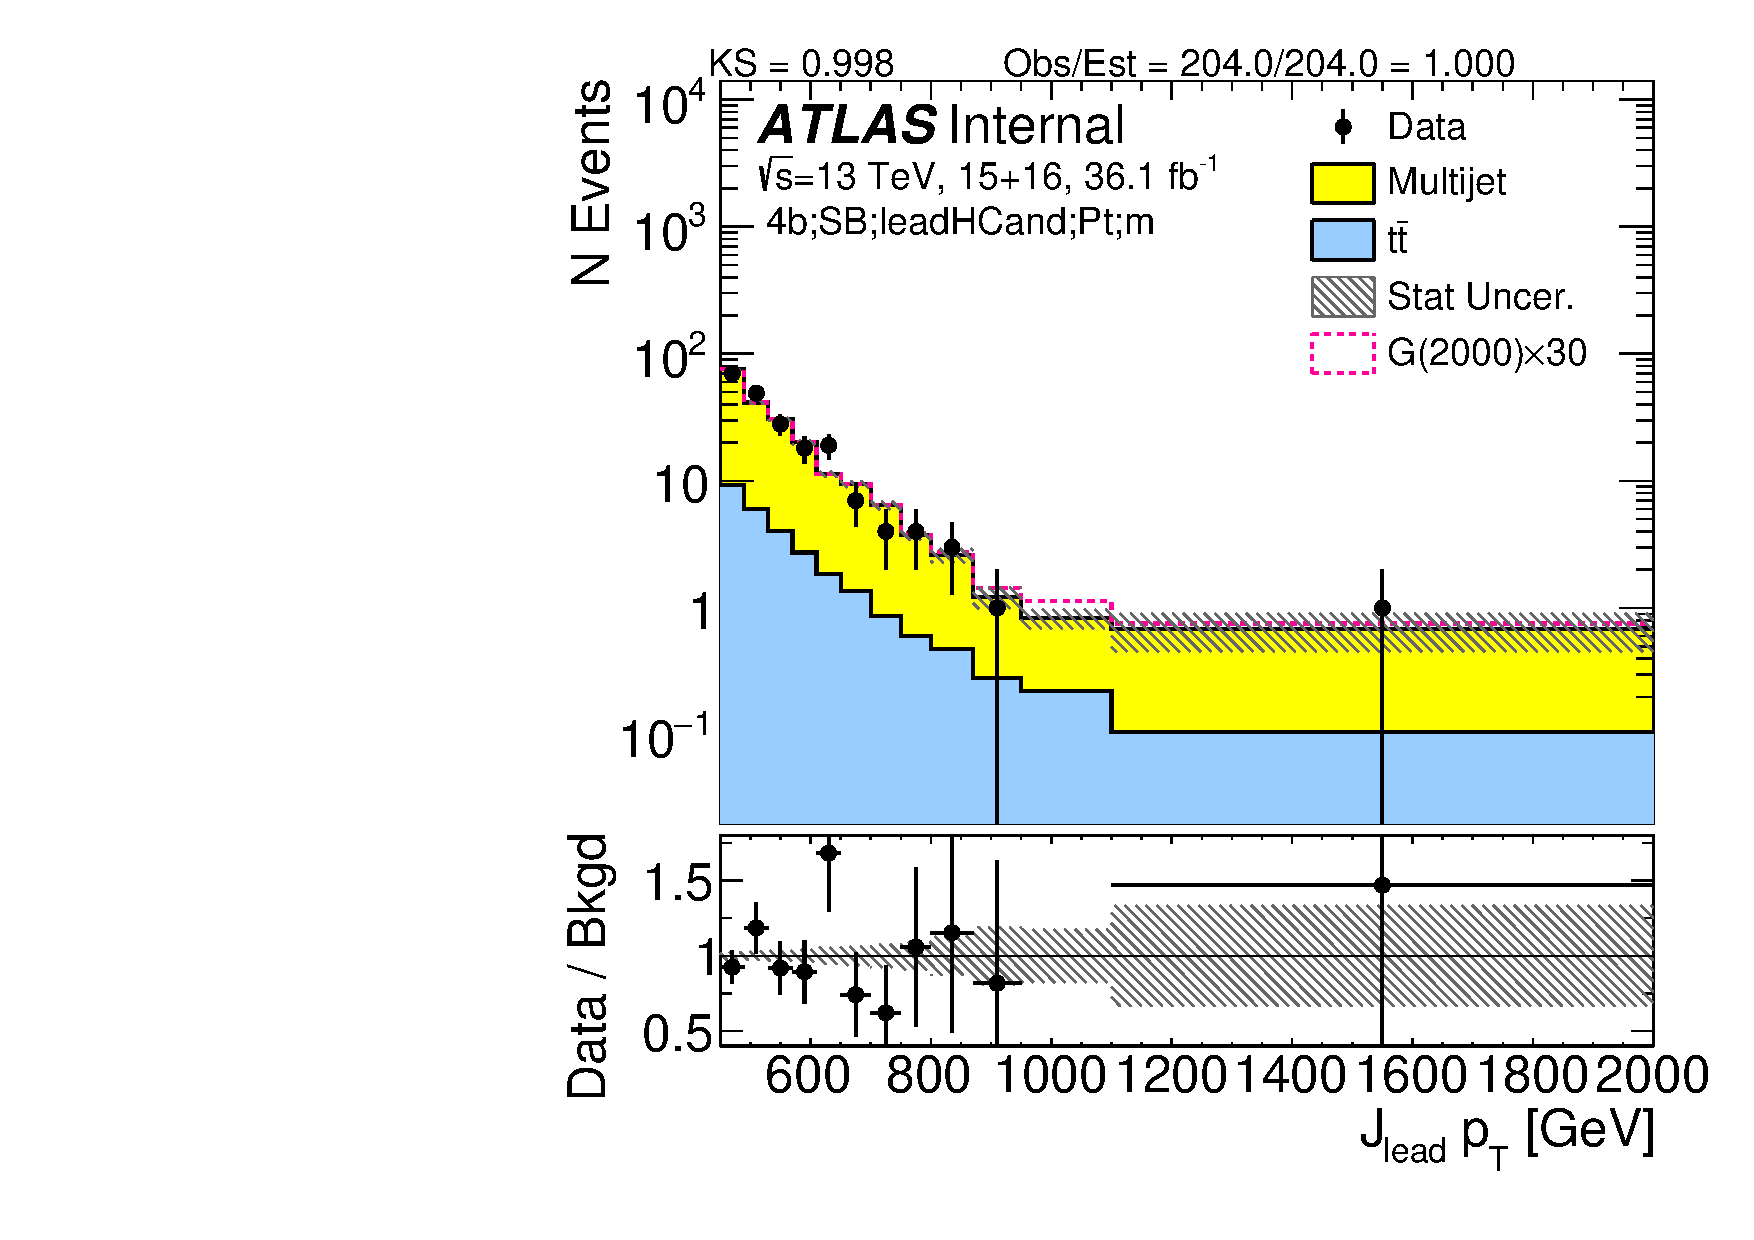
\includegraphics[width=0.32\textwidth,angle=-90]{figures/boosted/Sideband/b77_FourTag_Sideband_leadHCand_Pt_m_1.pdf}
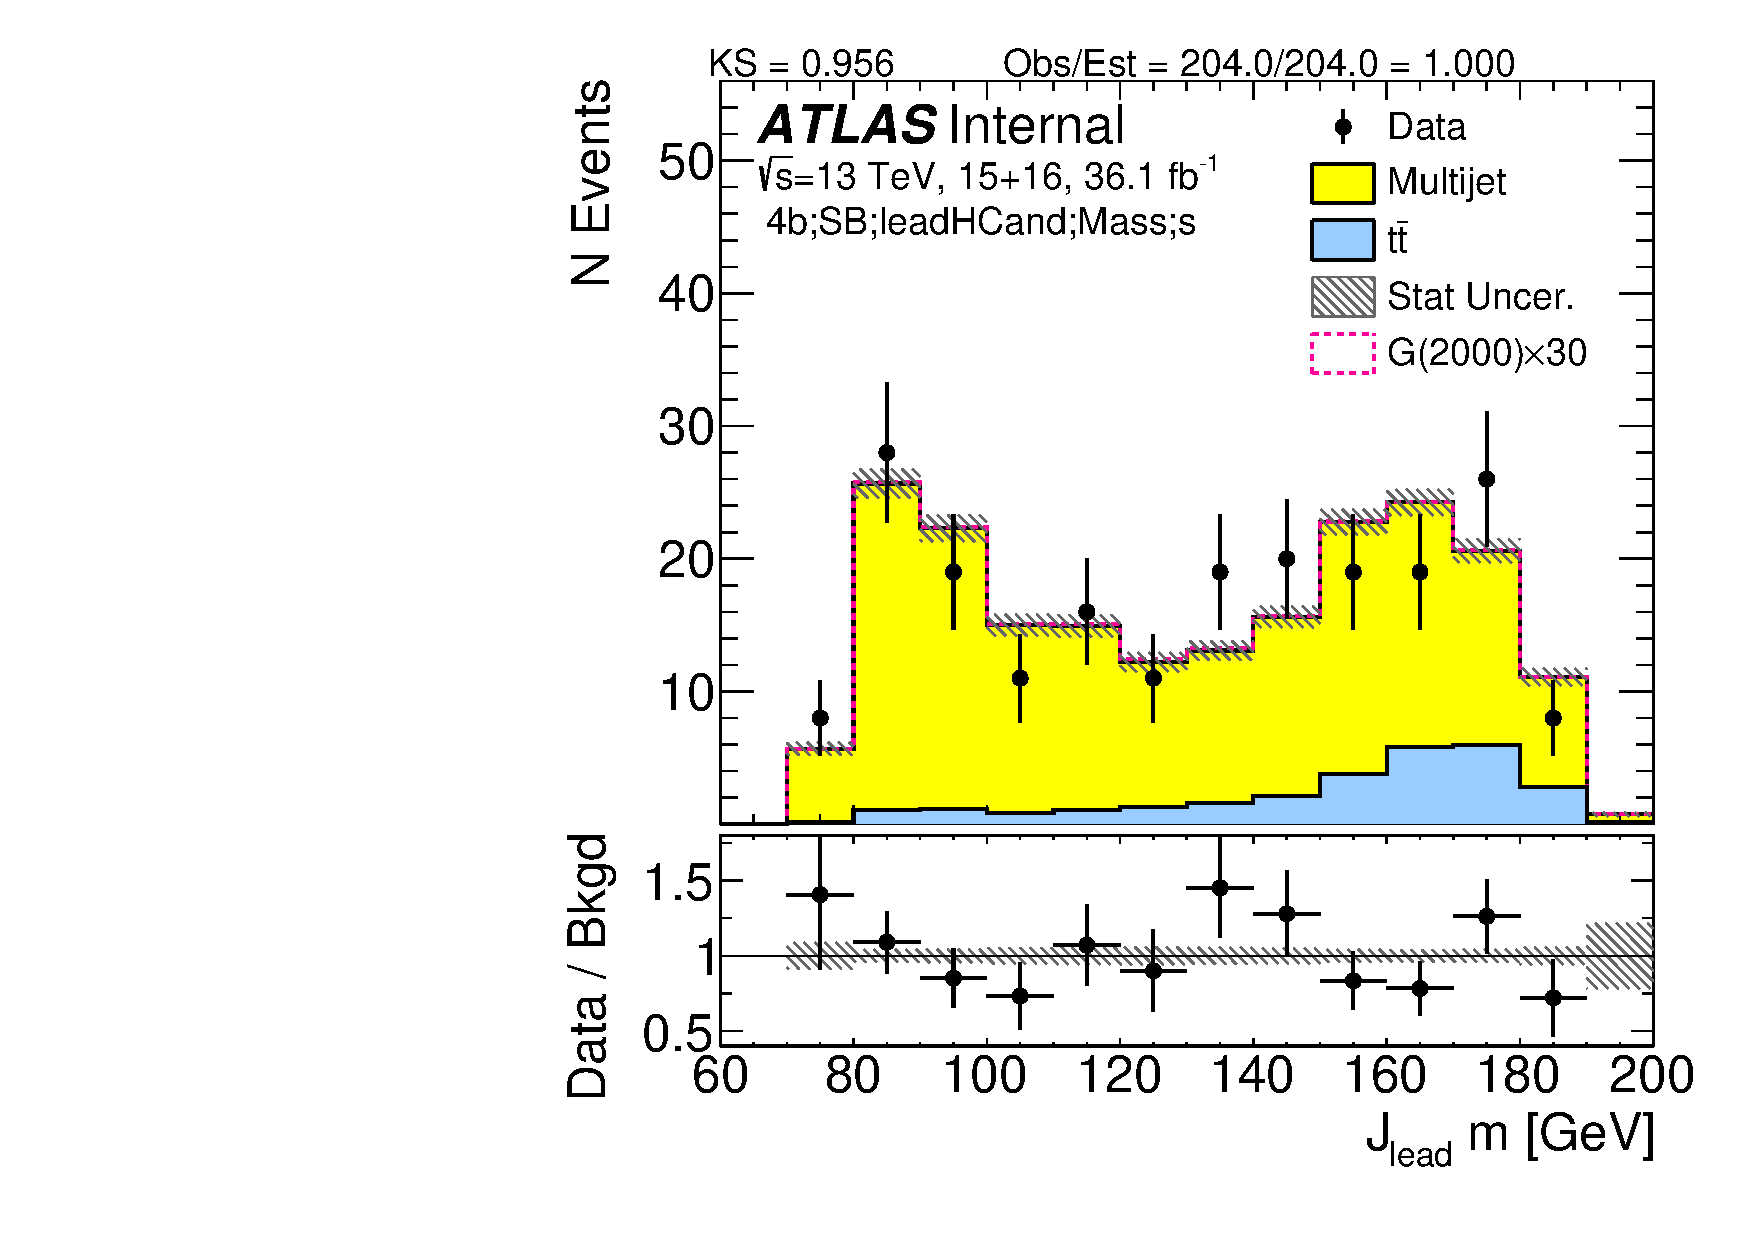
\includegraphics[width=0.32\textwidth,angle=-90]{figures/boosted/Sideband/b77_FourTag_Sideband_leadHCand_Mass_s.pdf}\\
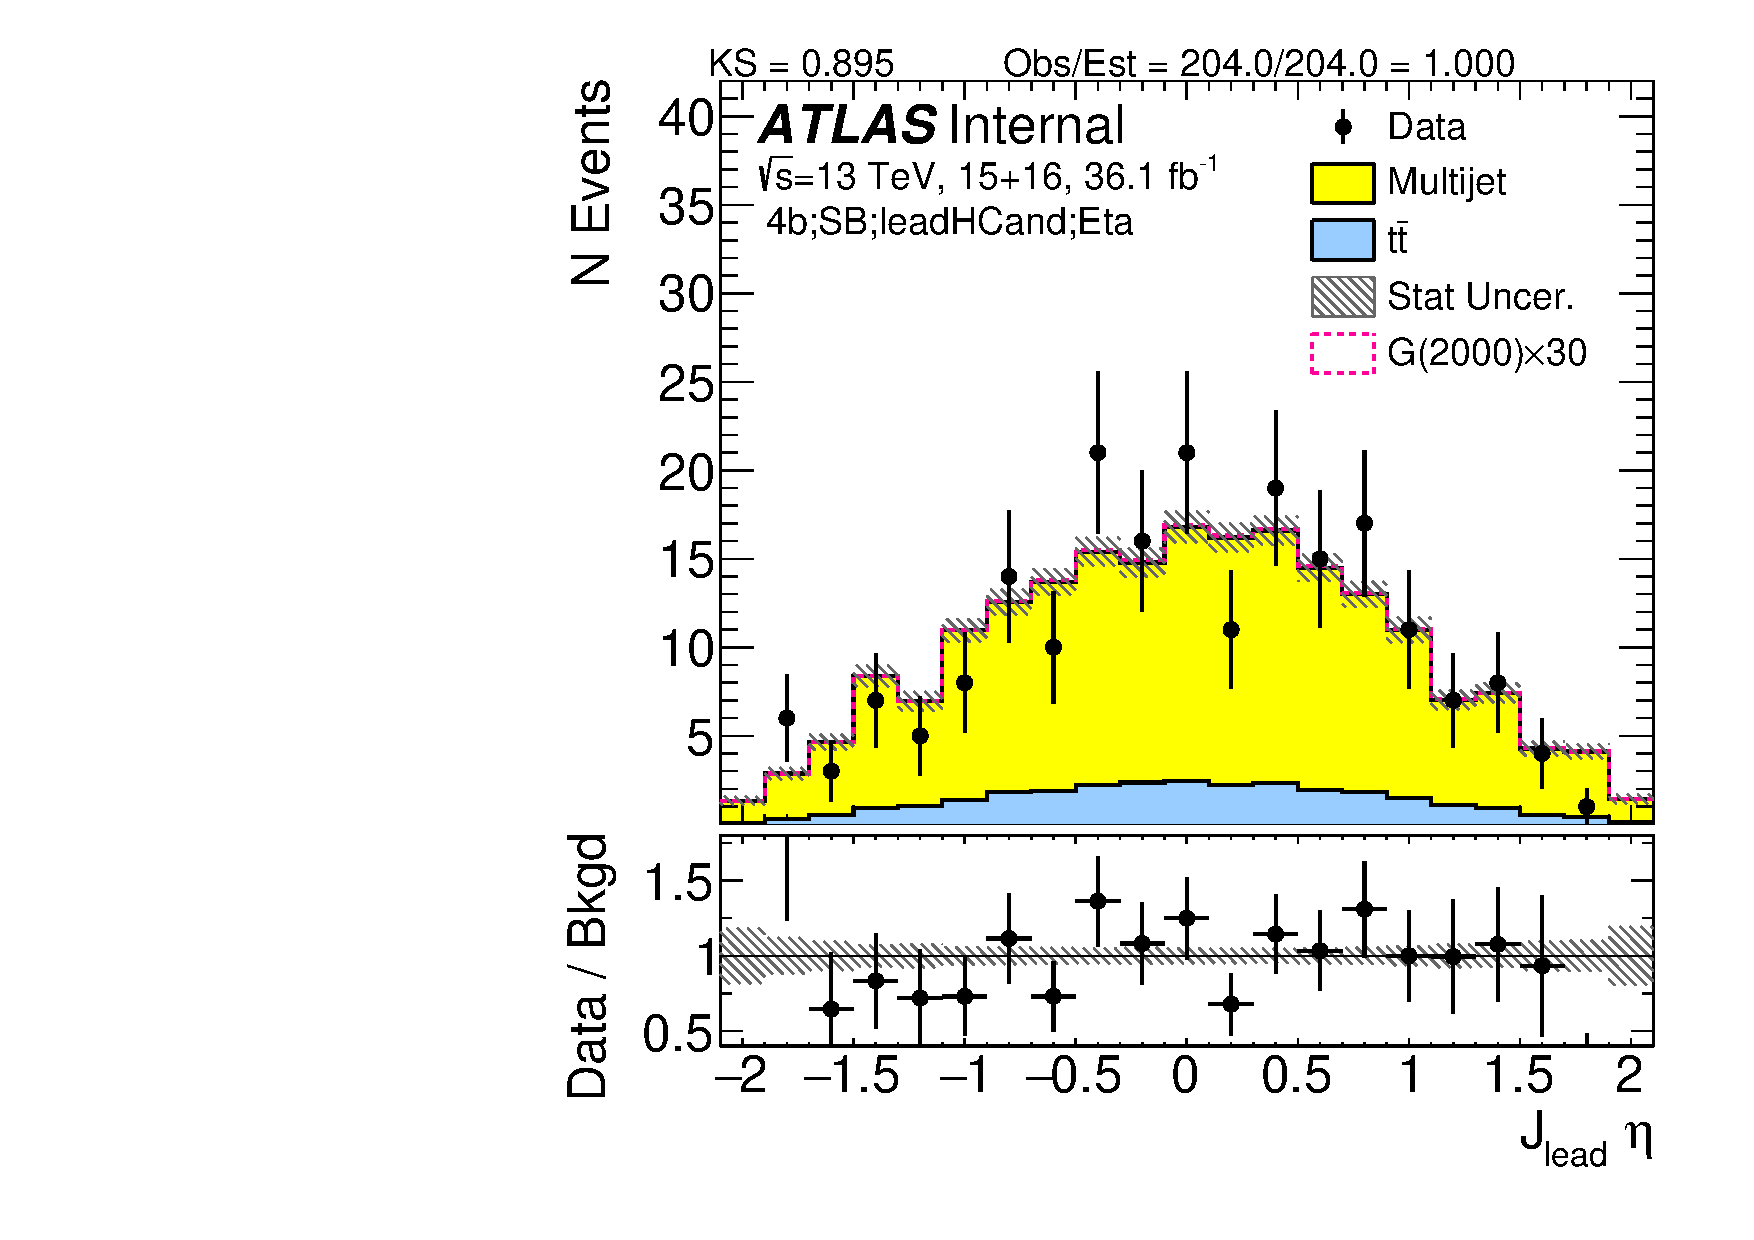
\includegraphics[width=0.32\textwidth,angle=-90]{figures/boosted/Sideband/b77_FourTag_Sideband_leadHCand_Eta.pdf}
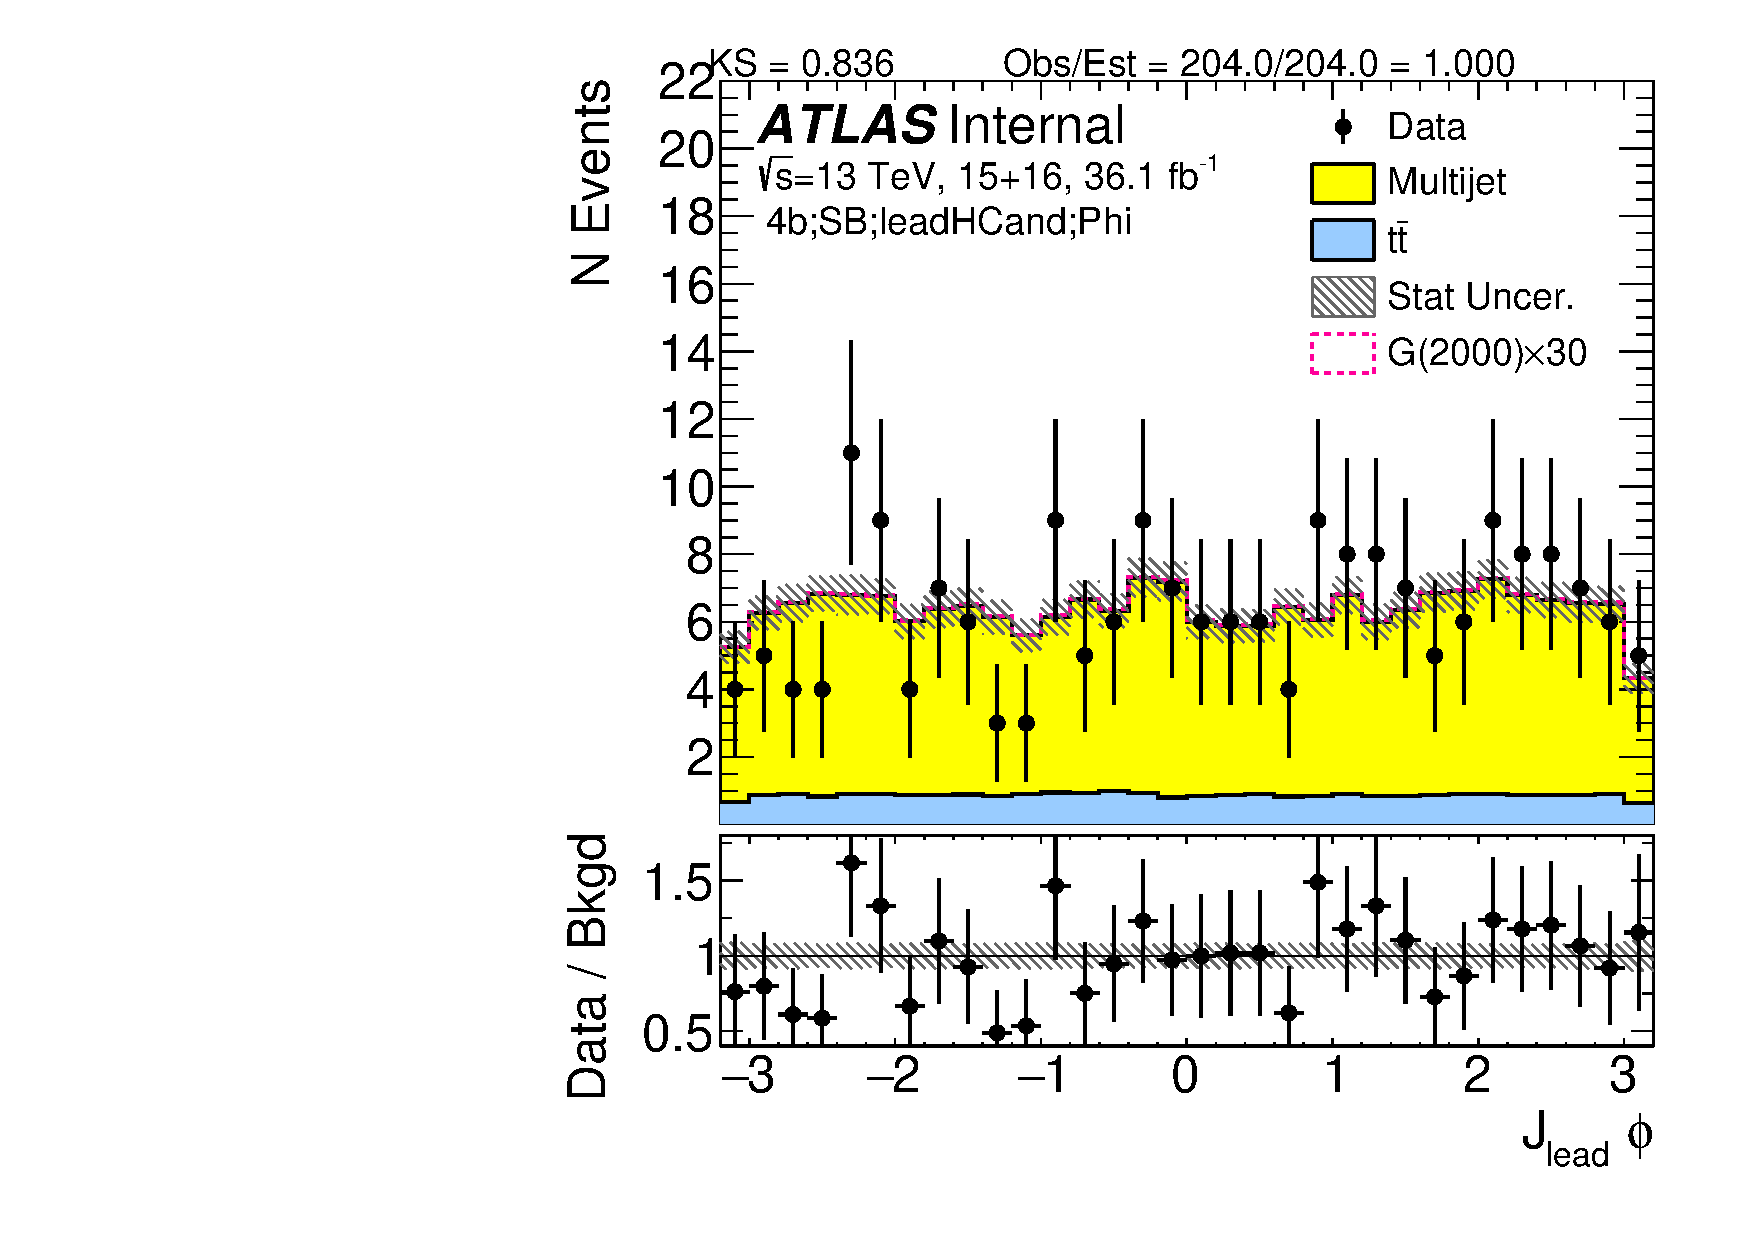
\includegraphics[width=0.32\textwidth,angle=-90]{figures/boosted/Sideband/b77_FourTag_Sideband_leadHCand_Phi.pdf}
  \caption{Kinematics (\pt~, mass, $\eta$, $\phi$) of the lead large-\R jet in data and prediction in the sideband region after requiring 4 $b$-tags.}
  \label{fig:boosted-4b-sideband-ak10-lead}
\end{center}
\end{figure*}

\begin{figure*}[htbp!]
\begin{center}
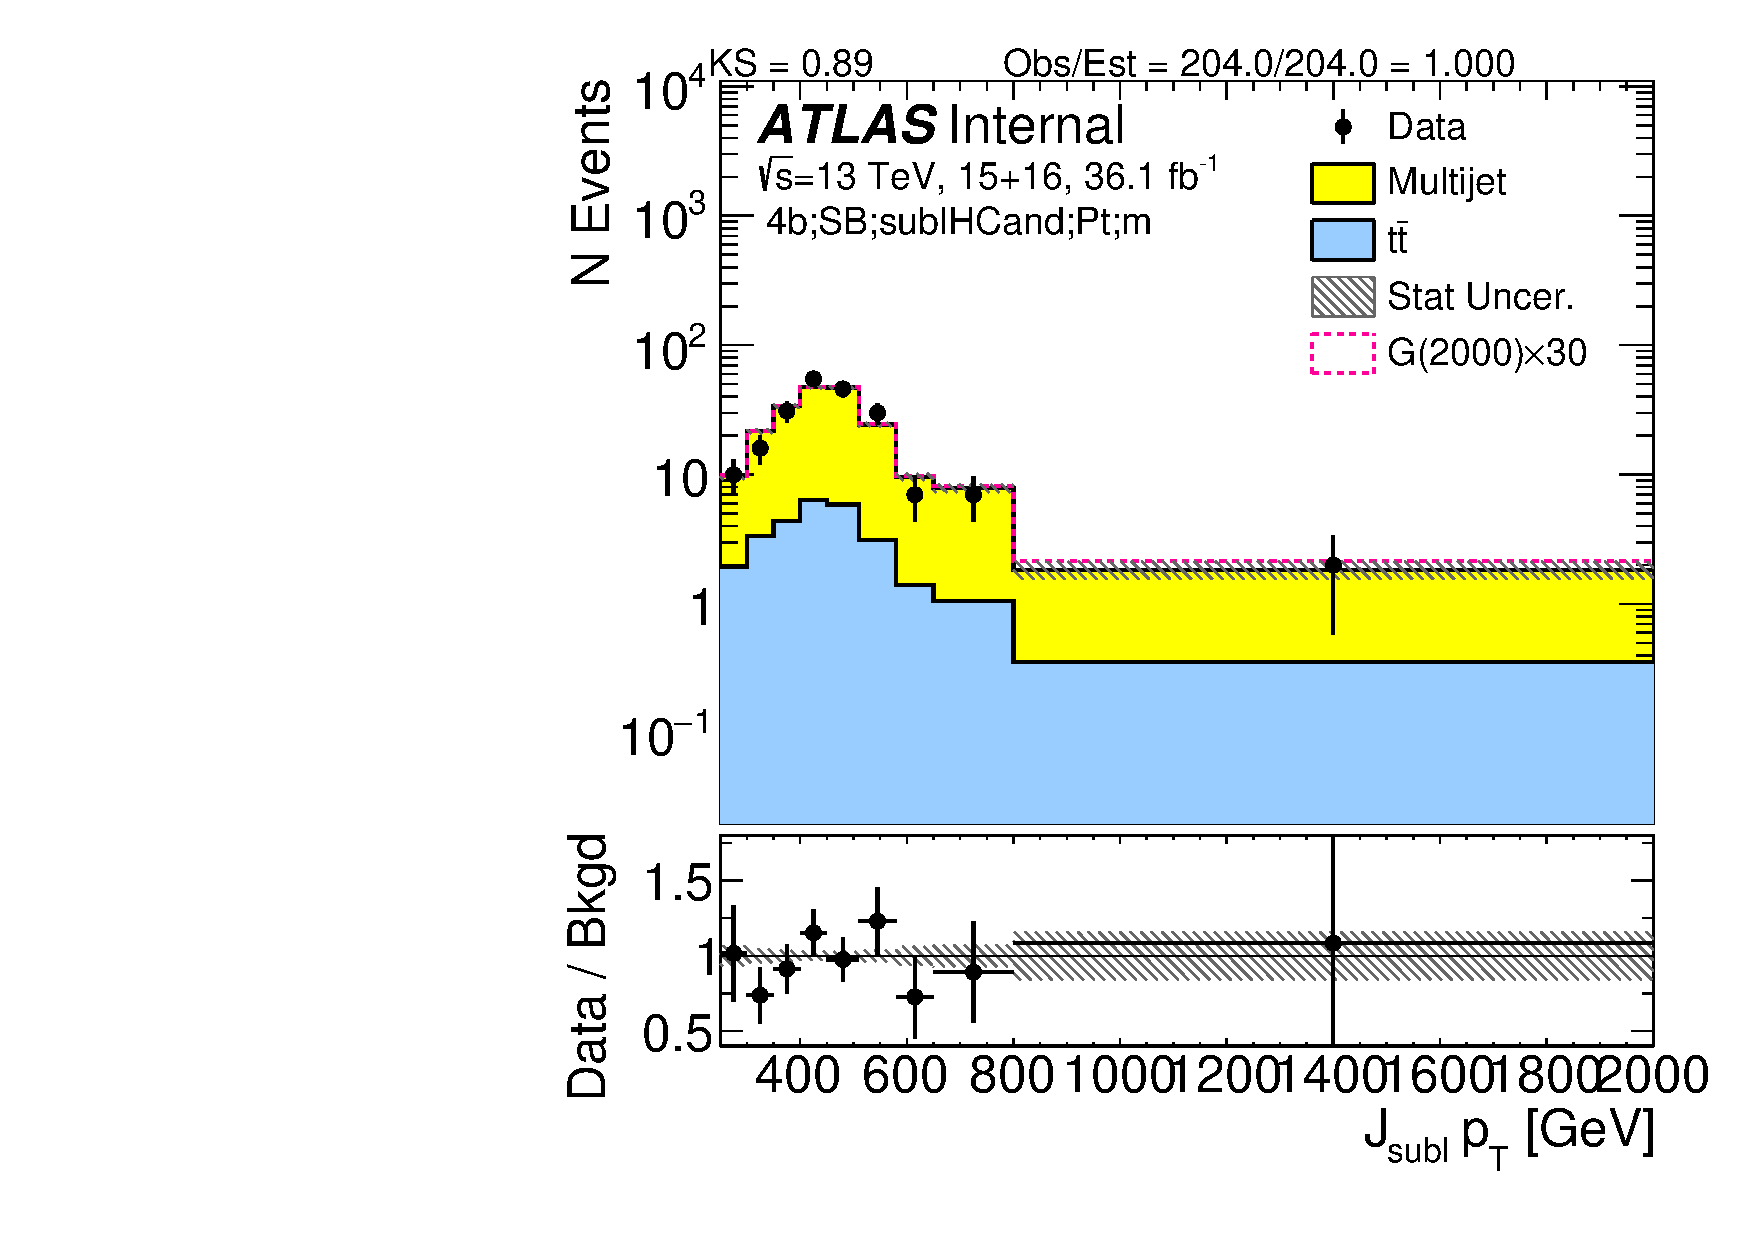
\includegraphics[width=0.32\textwidth,angle=-90]{figures/boosted/Sideband/b77_FourTag_Sideband_sublHCand_Pt_m_1.pdf}
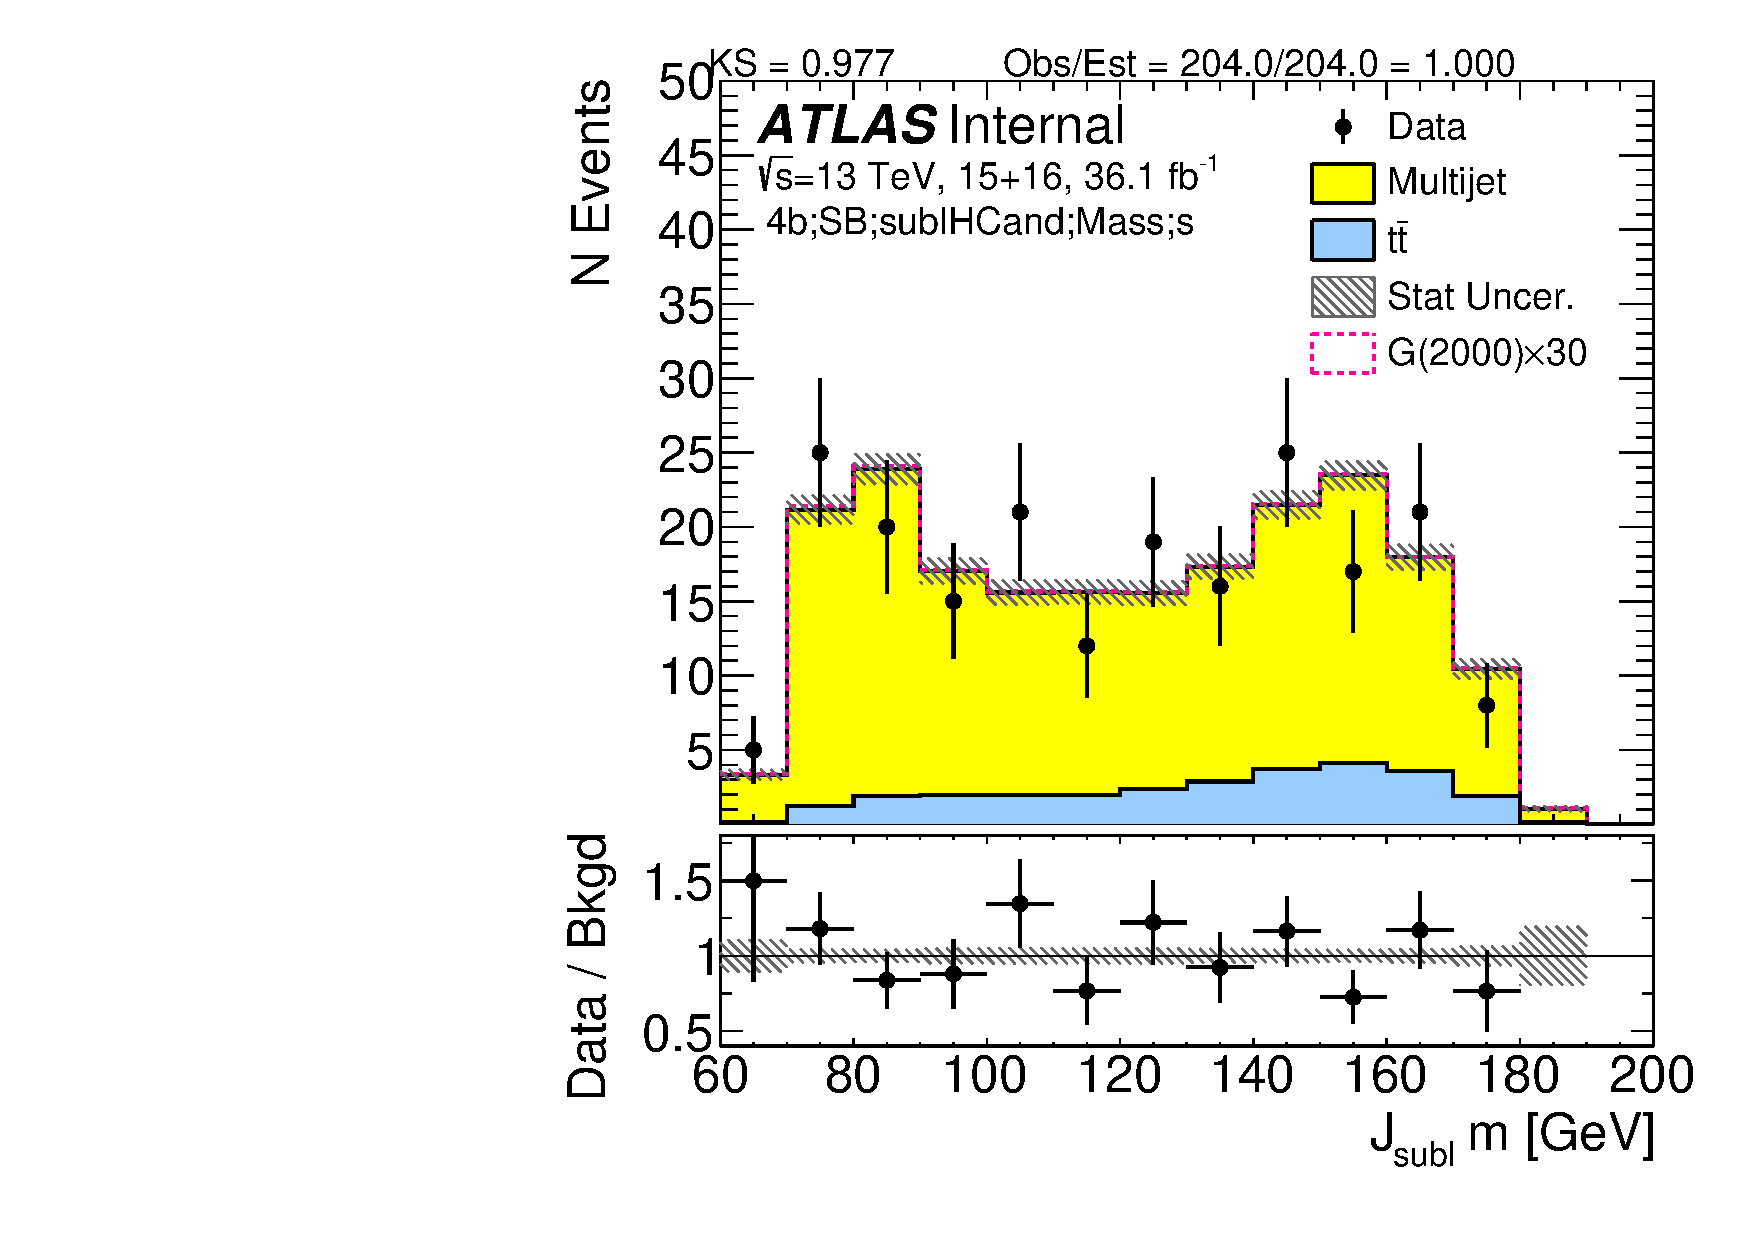
\includegraphics[width=0.32\textwidth,angle=-90]{figures/boosted/Sideband/b77_FourTag_Sideband_sublHCand_Mass_s.pdf}\\
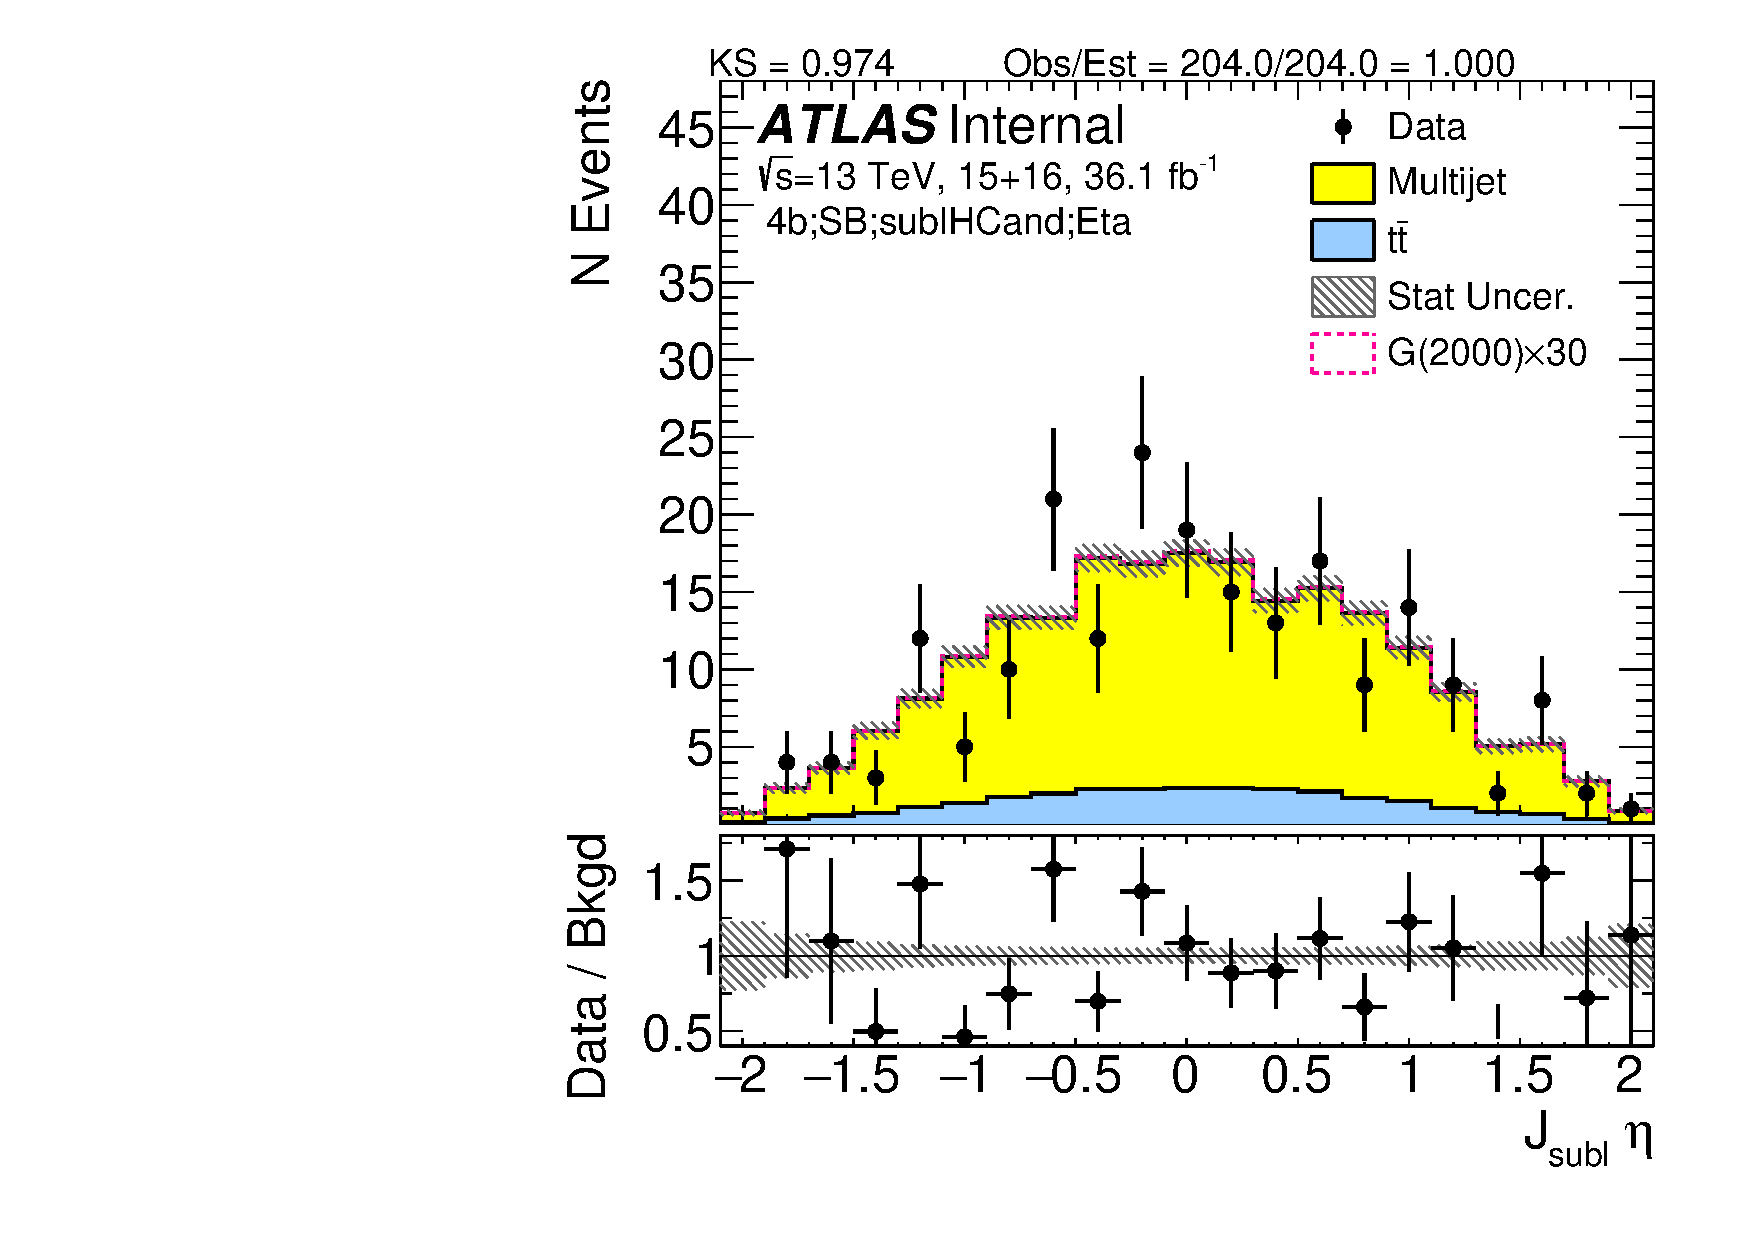
\includegraphics[width=0.32\textwidth,angle=-90]{figures/boosted/Sideband/b77_FourTag_Sideband_sublHCand_Eta.pdf}
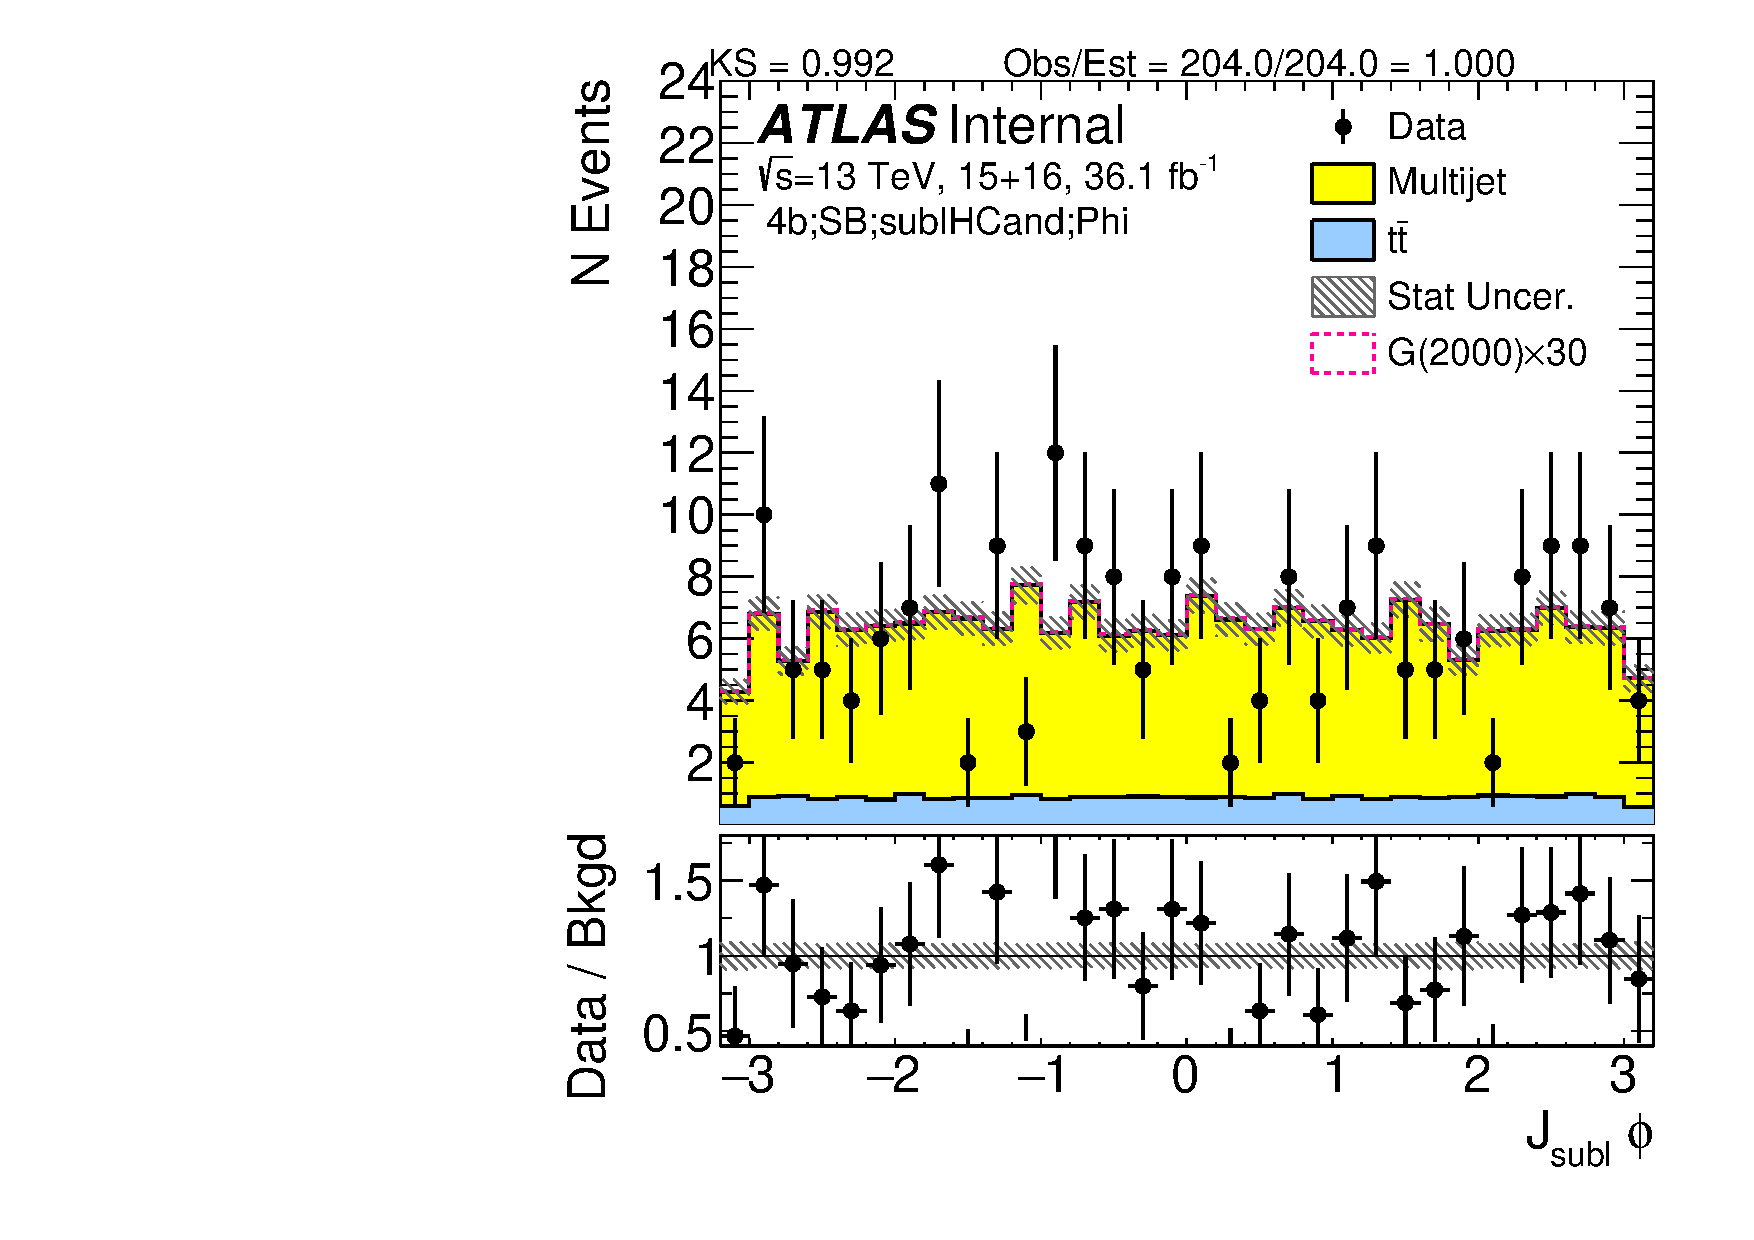
\includegraphics[width=0.32\textwidth,angle=-90]{figures/boosted/Sideband/b77_FourTag_Sideband_sublHCand_Phi.pdf}
  \caption{Kinematics (\pt~, mass, $\eta$, $\phi$) of the subleading large-\R jet in data and prediction in the sideband region after requiring 4 $b$-tags.}
  \label{fig:boosted-4b-sideband-ak10-subl}
\end{center}
\end{figure*}

\begin{figure*}[htbp!]
\begin{center}
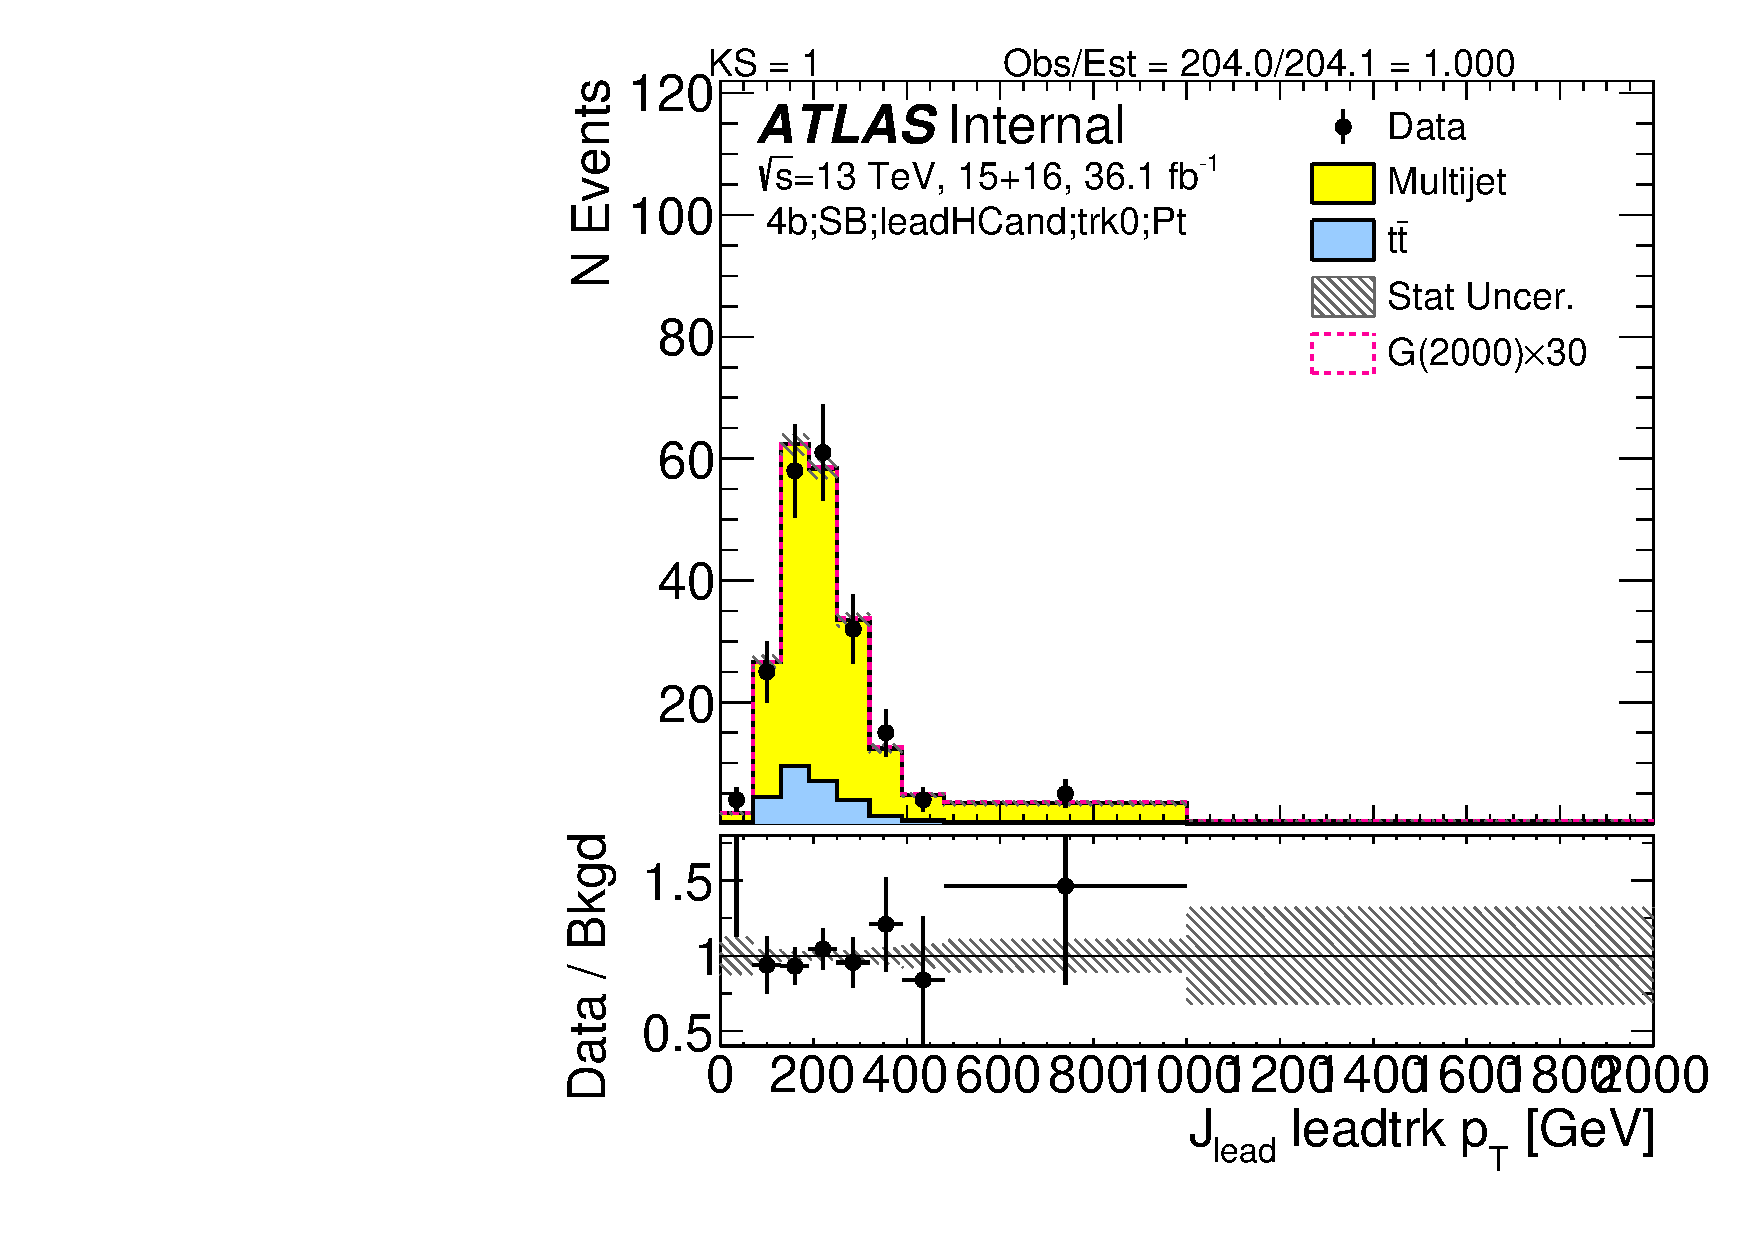
\includegraphics[width=0.32\textwidth,angle=-90]{figures/boosted/Sideband/b77_FourTag_Sideband_leadHCand_trk0_Pt.pdf}
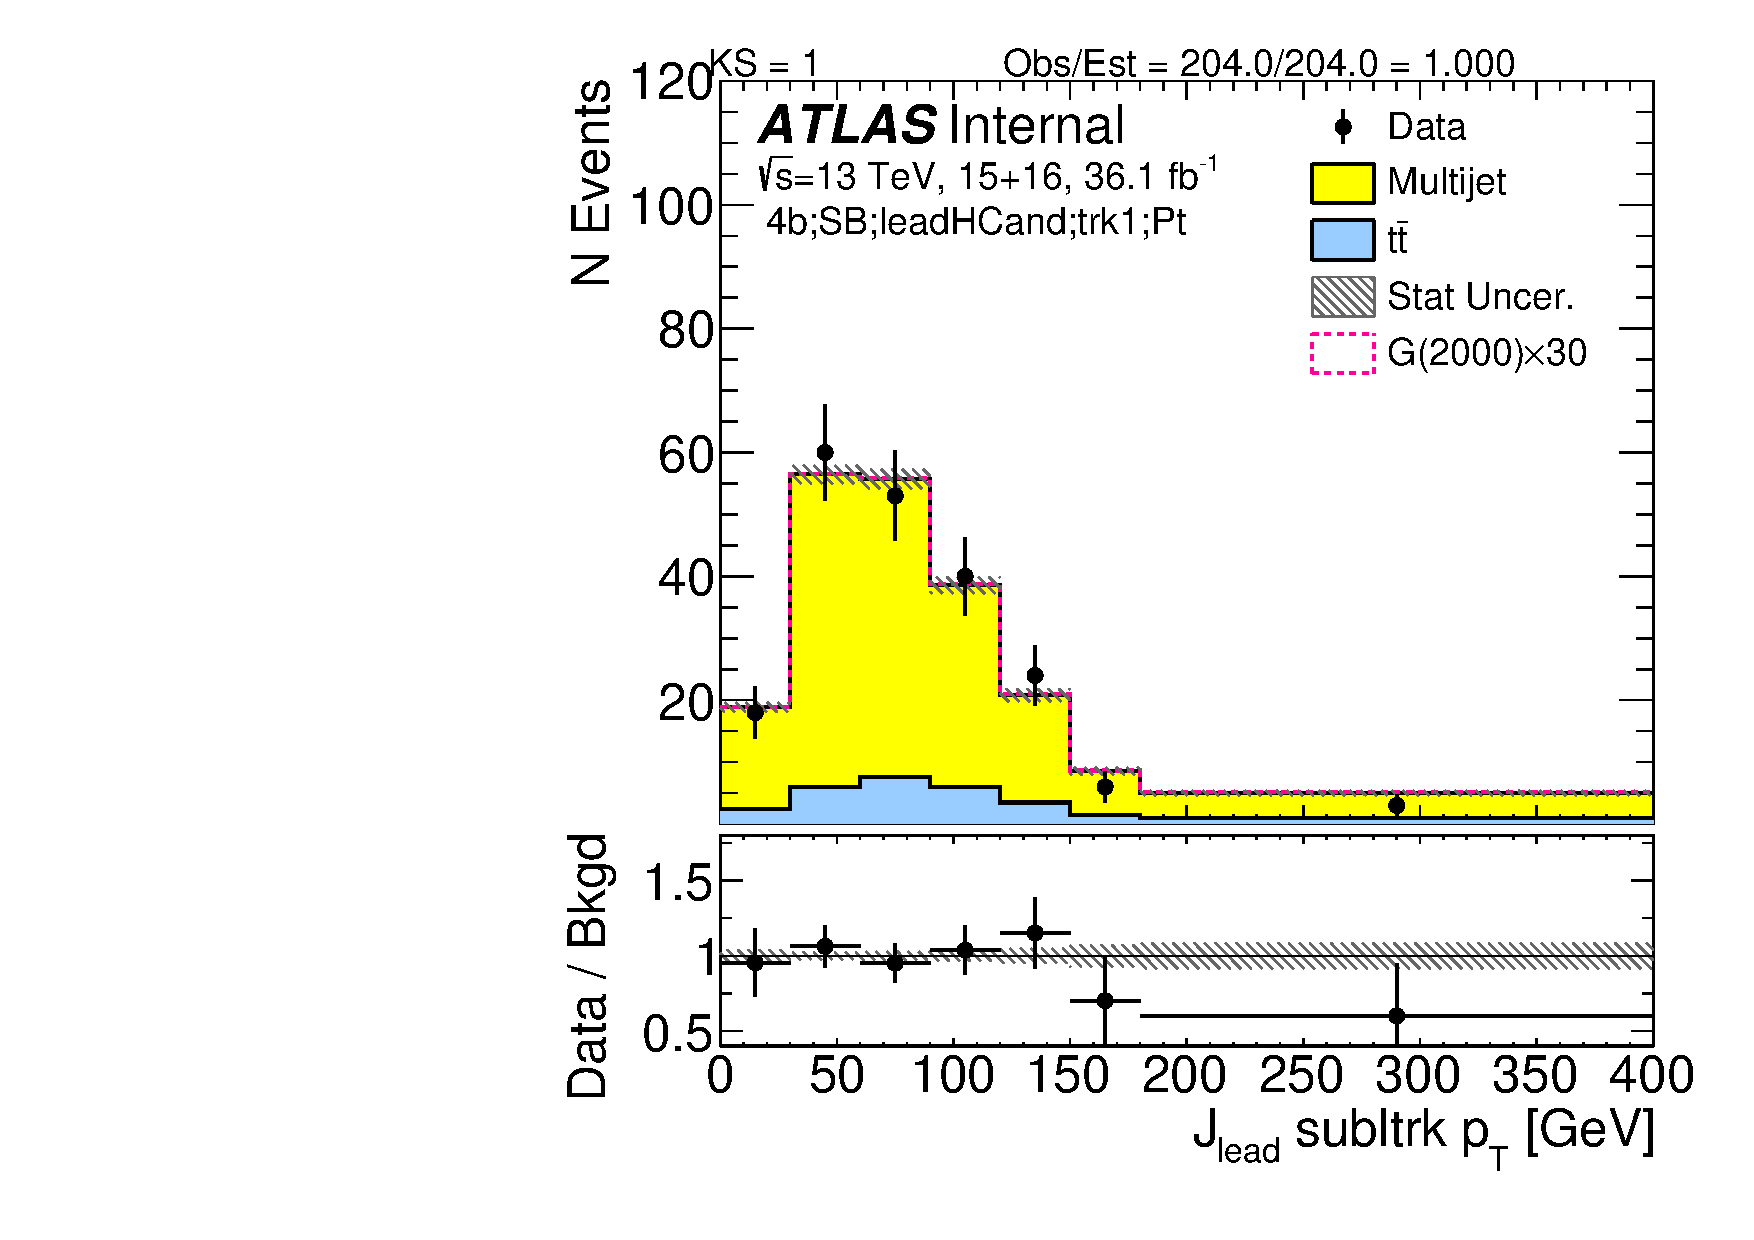
\includegraphics[width=0.32\textwidth,angle=-90]{figures/boosted/Sideband/b77_FourTag_Sideband_leadHCand_trk1_Pt.pdf}\\
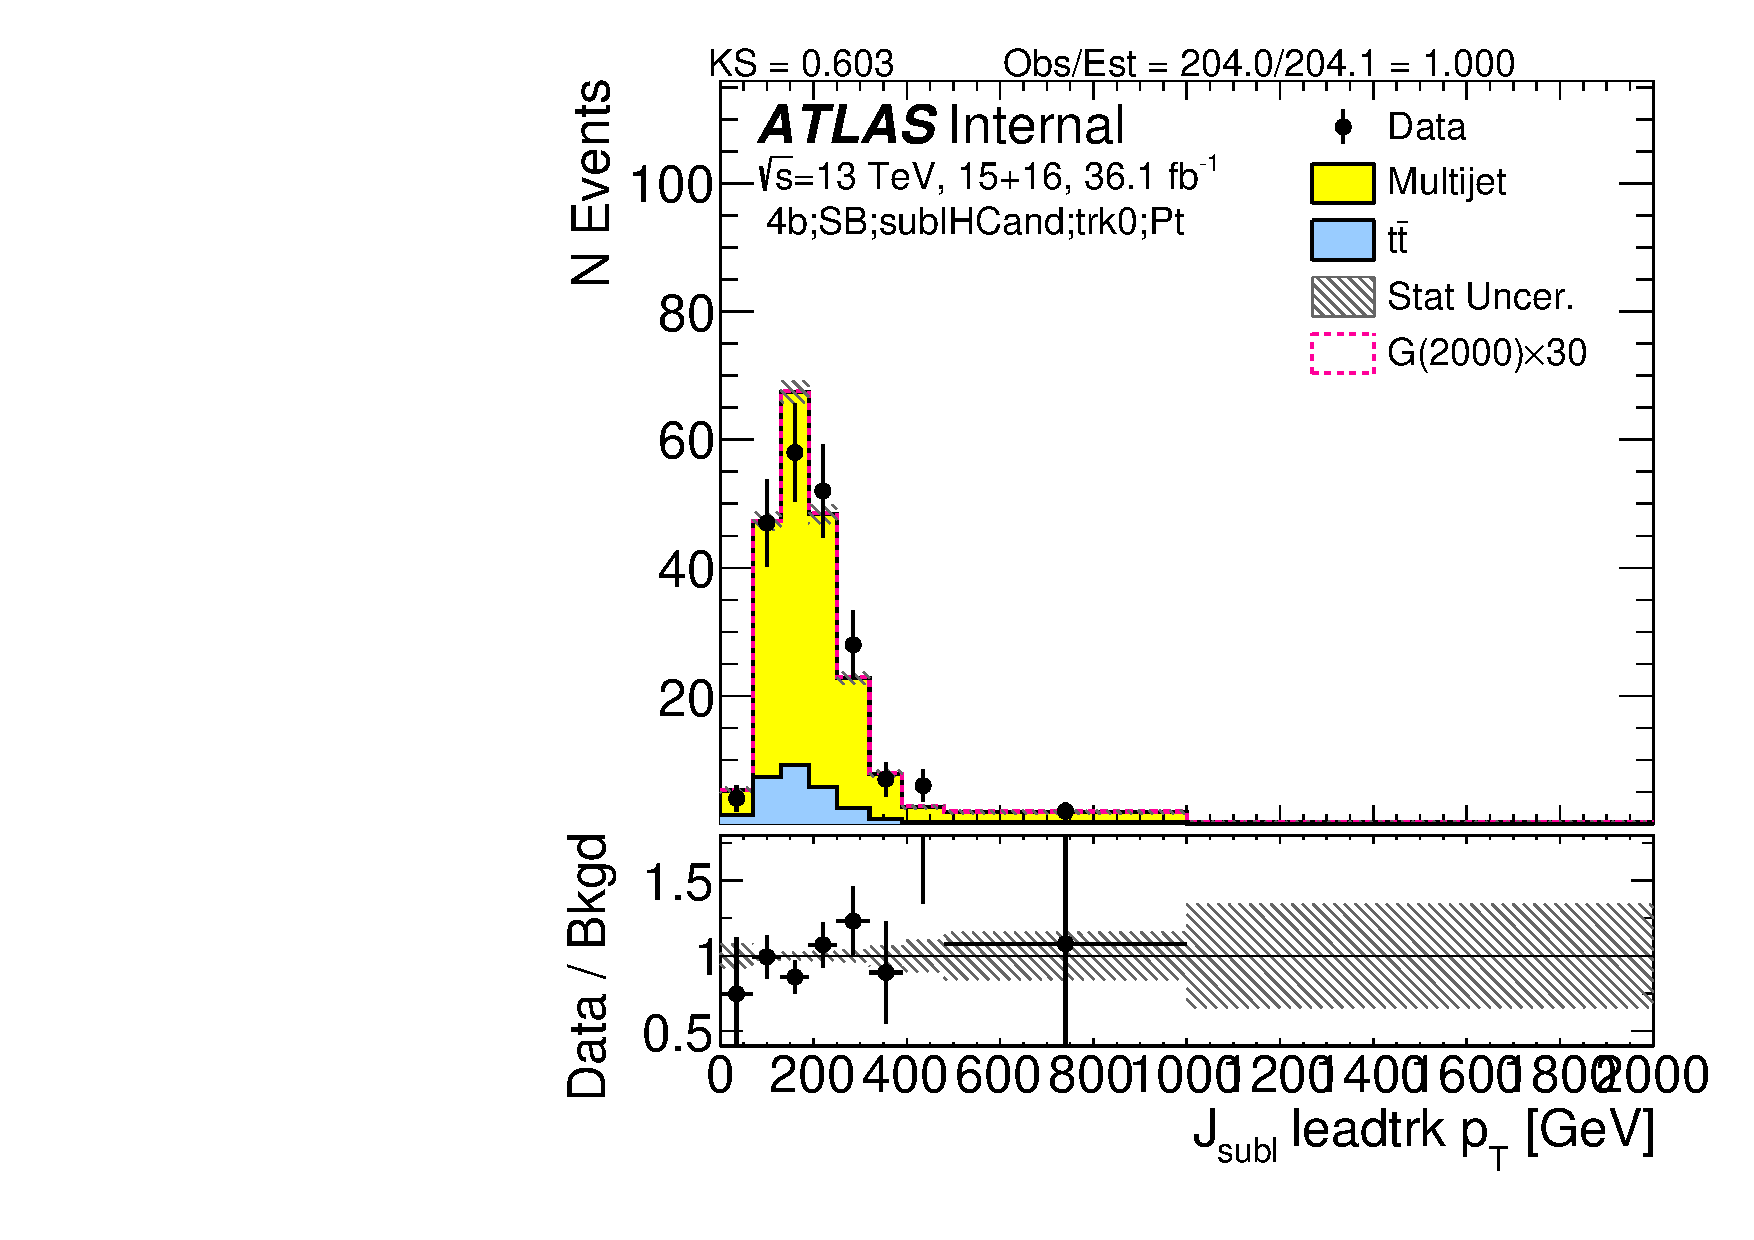
\includegraphics[width=0.32\textwidth,angle=-90]{figures/boosted/Sideband/b77_FourTag_Sideband_sublHCand_trk0_Pt.pdf}
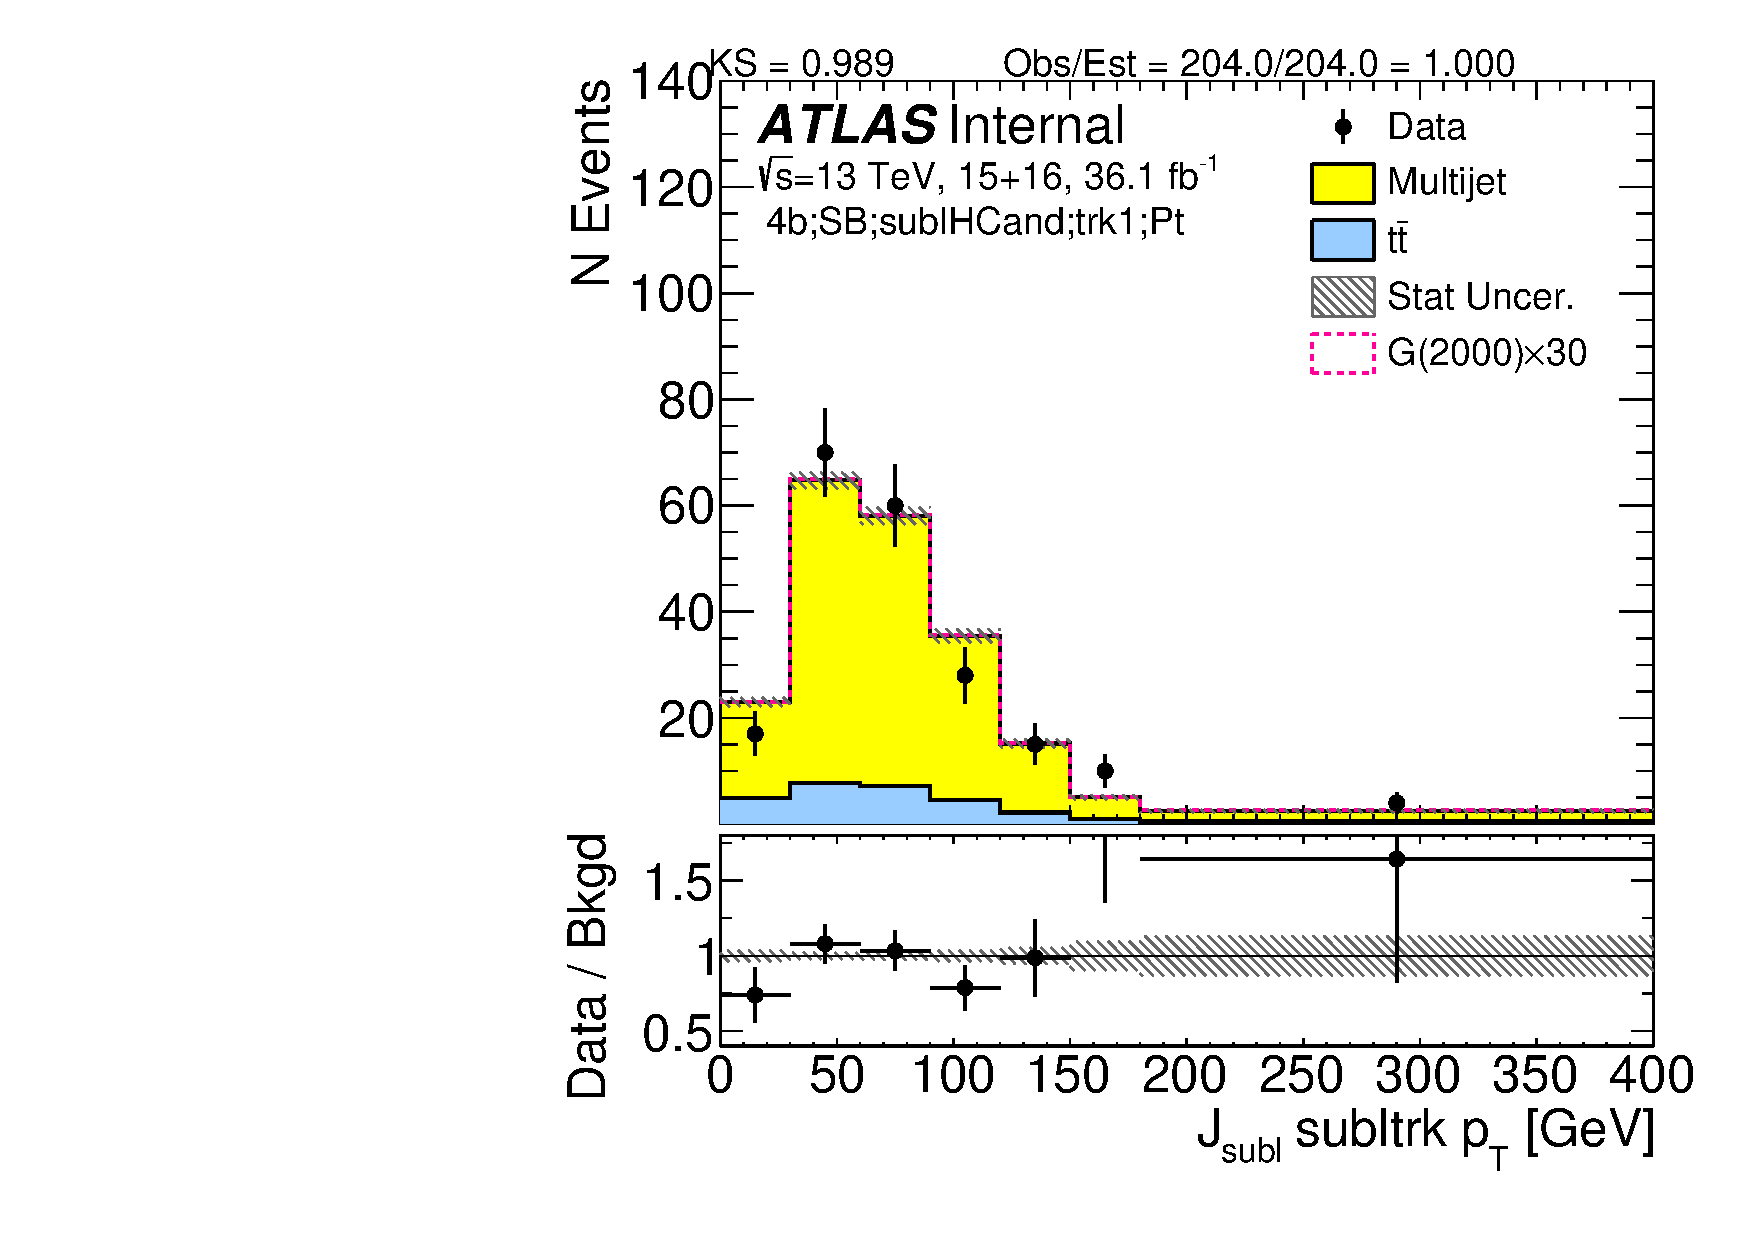
\includegraphics[width=0.32\textwidth,angle=-90]{figures/boosted/Sideband/b77_FourTag_Sideband_sublHCand_trk1_Pt.pdf}\\
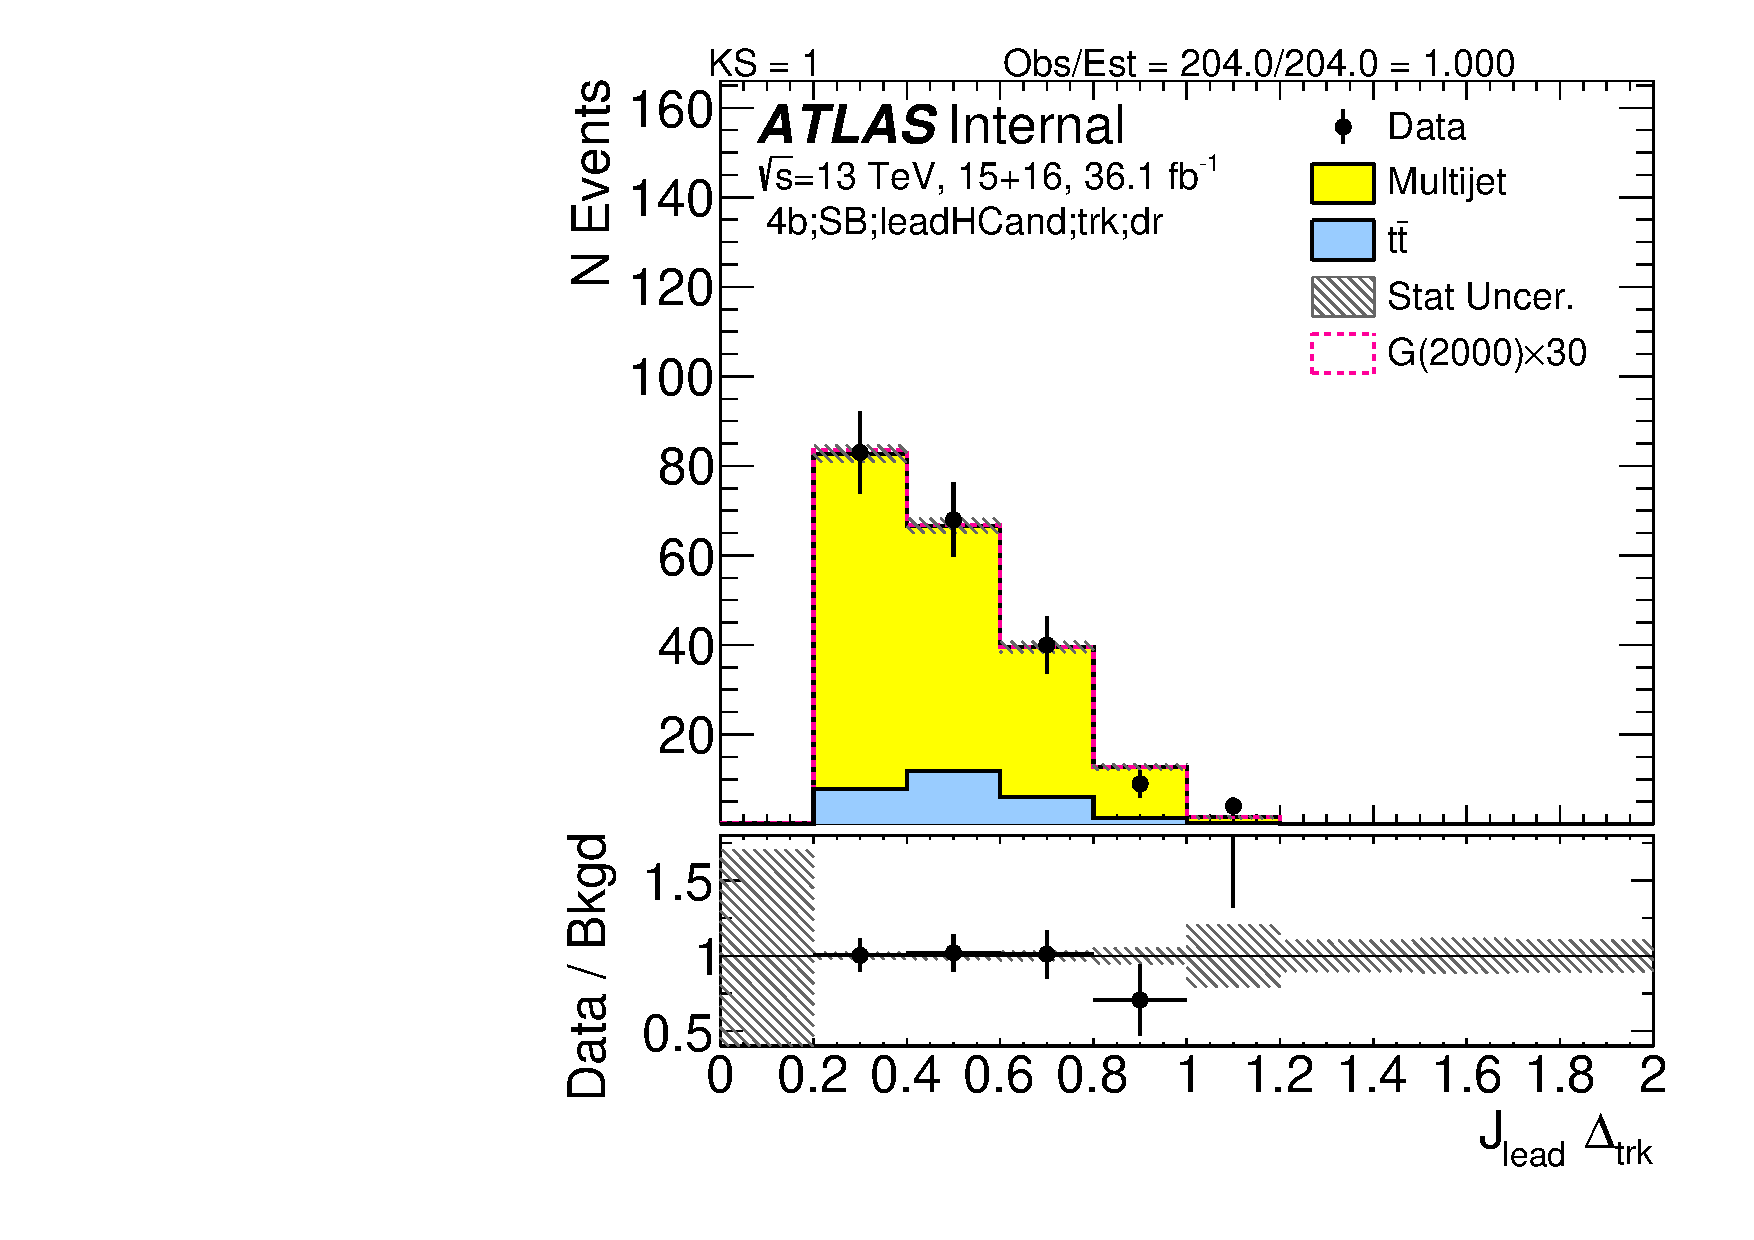
\includegraphics[width=0.32\textwidth,angle=-90]{figures/boosted/Sideband/b77_FourTag_Sideband_leadHCand_trk_dr.pdf}
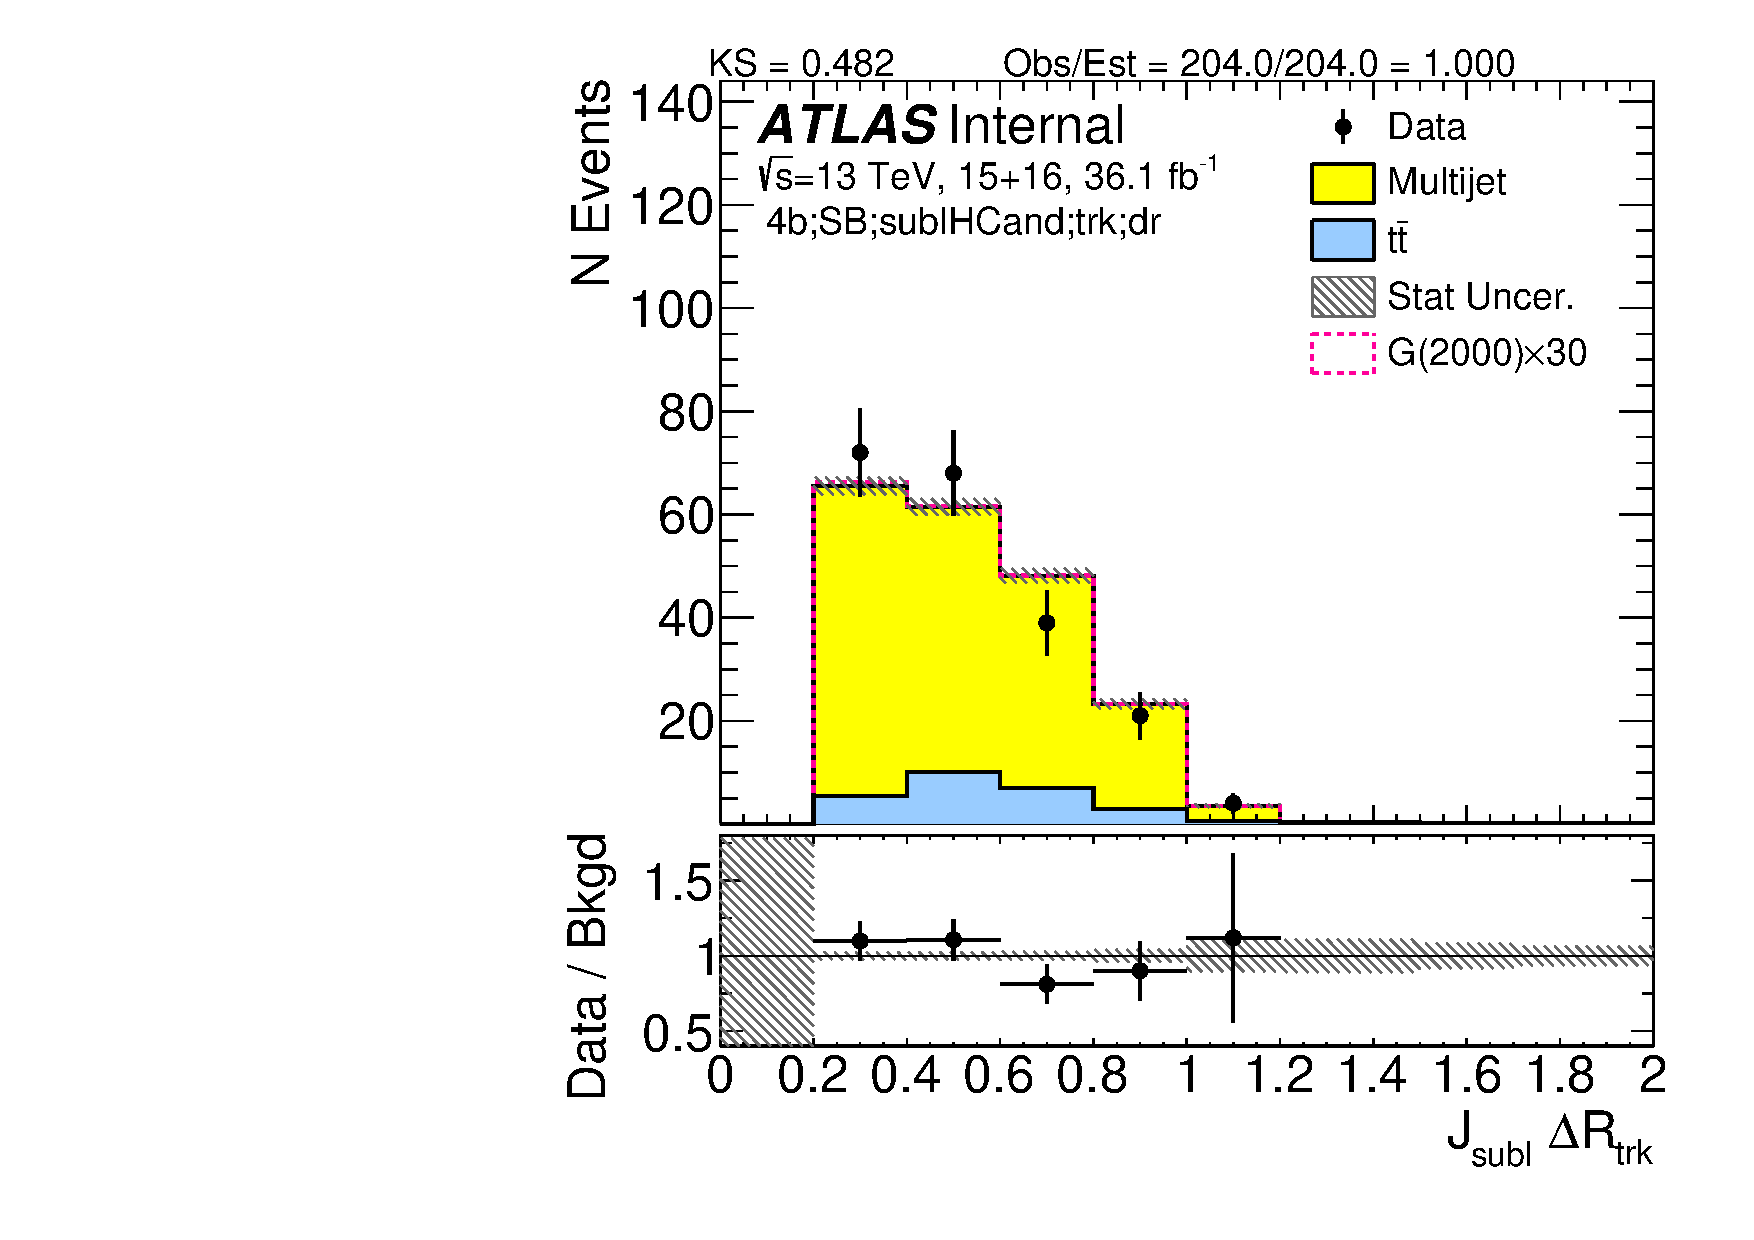
\includegraphics[width=0.32\textwidth,angle=-90]{figures/boosted/Sideband/b77_FourTag_Sideband_sublHCand_trk_dr.pdf}
  \caption{First two rows show the \pt~ of the lead (left) and sub-lead (right) small-$R$ track jets associated to the lead (first-row) and sub-lead (second-row) large-\R jet in data and prediction in the sideband region after requiring 4 $b$-tags. Third row shows the $\Delta R$ between two leading small-$R$ track-jets associated to the leading (left) and sub-leading (right) large-\R jet. }
  \label{fig:boosted-4b-sideband-ak2}
\end{center}
\end{figure*}


\begin{figure*}[htbp!]
\begin{center}
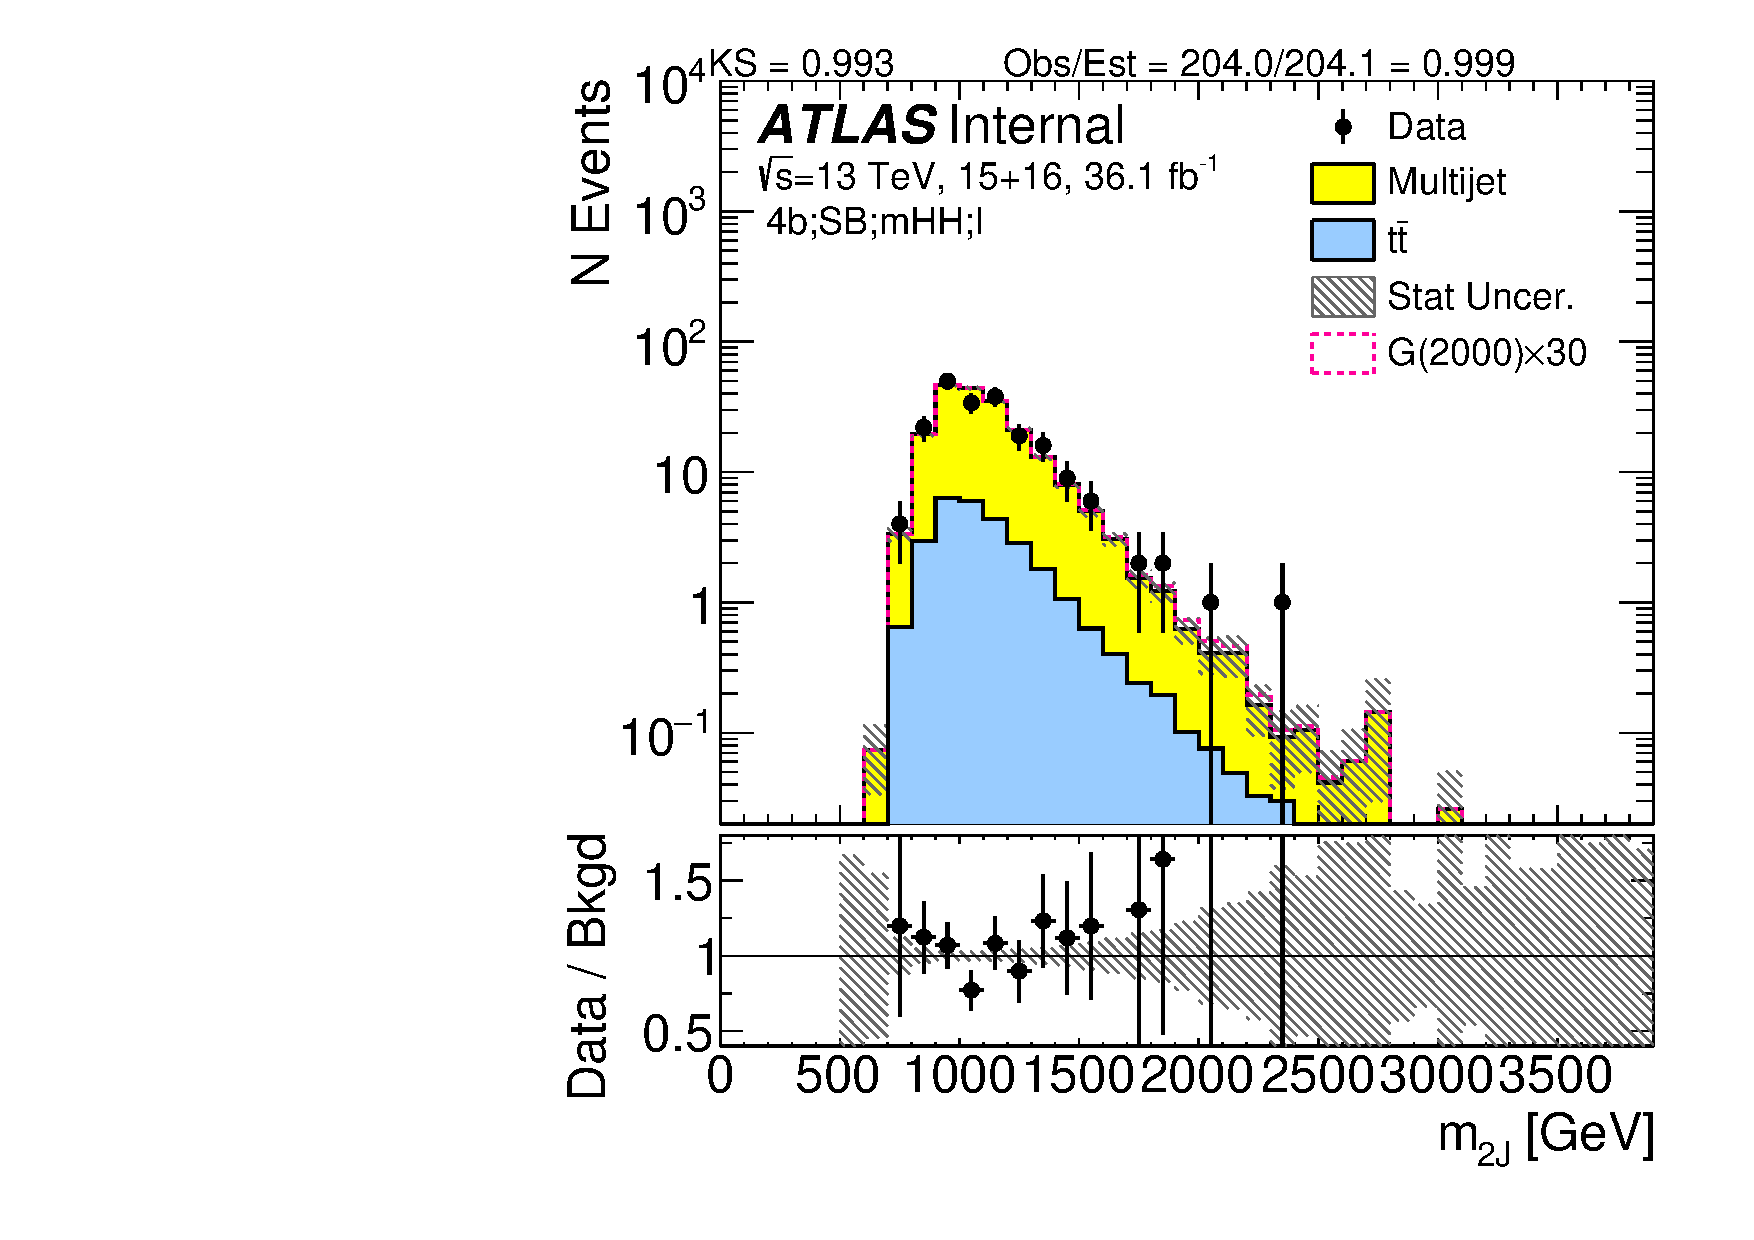
\includegraphics[width=0.32\textwidth,angle=-90]{figures/boosted/Sideband/b77_FourTag_Sideband_mHH_l_1.pdf}
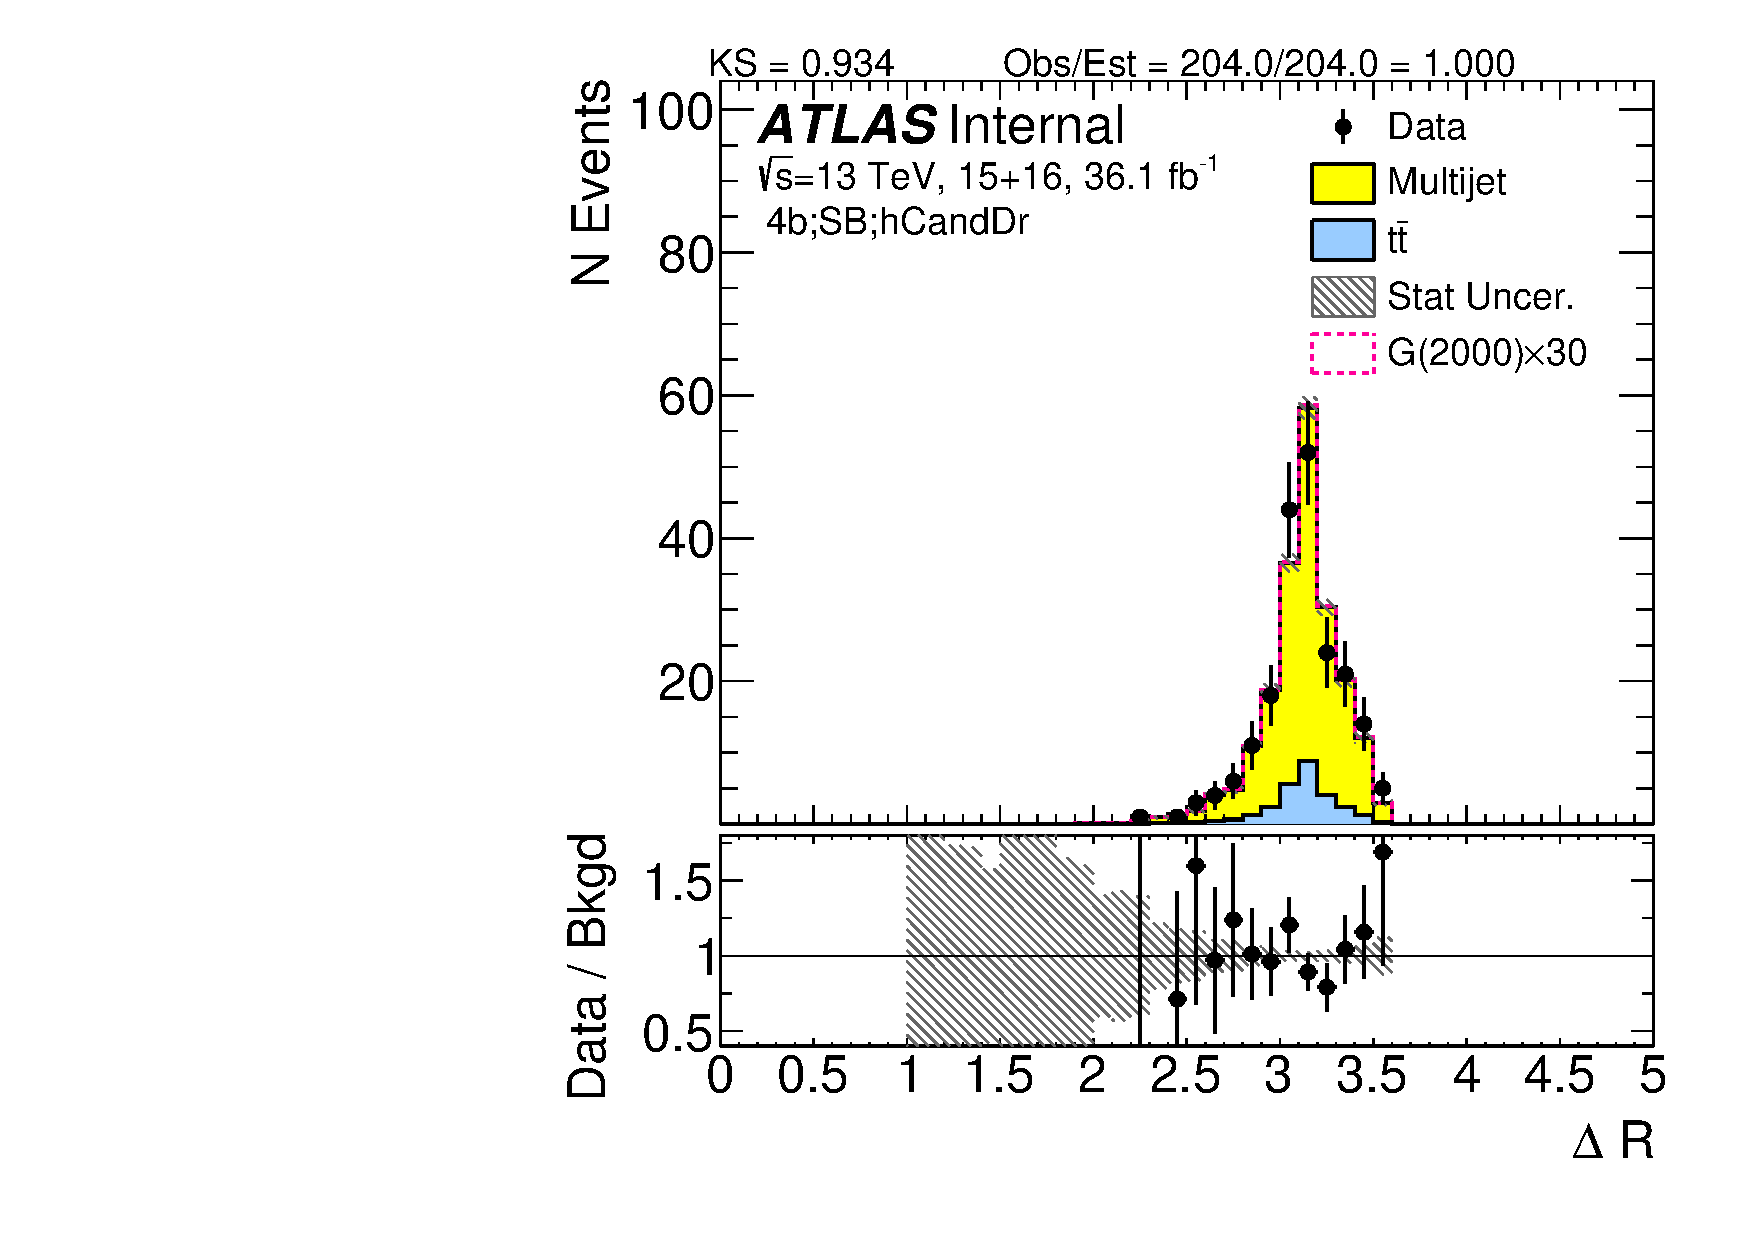
\includegraphics[width=0.32\textwidth,angle=-90]{figures/boosted/Sideband/b77_FourTag_Sideband_hCandDr.pdf}\\
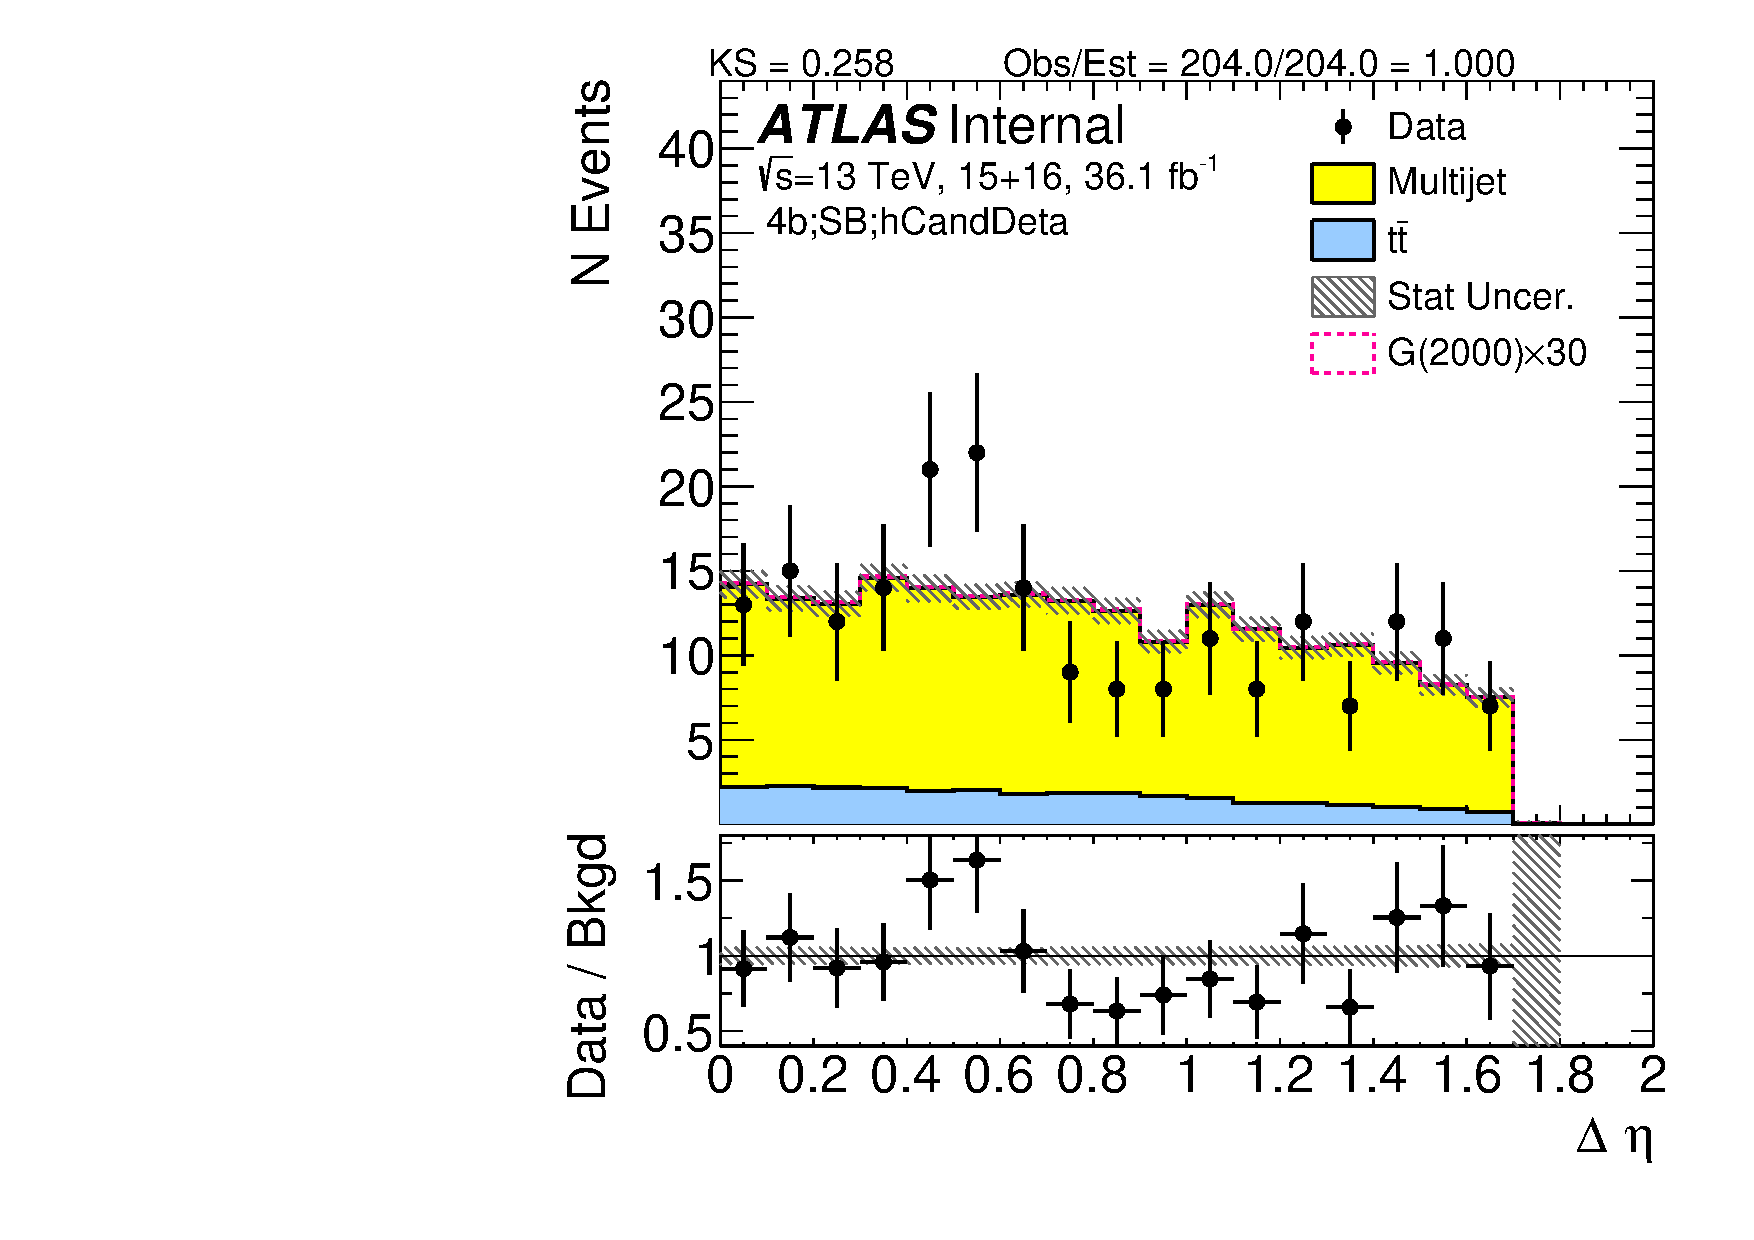
\includegraphics[width=0.32\textwidth,angle=-90]{figures/boosted/Sideband/b77_FourTag_Sideband_hCandDeta.pdf}
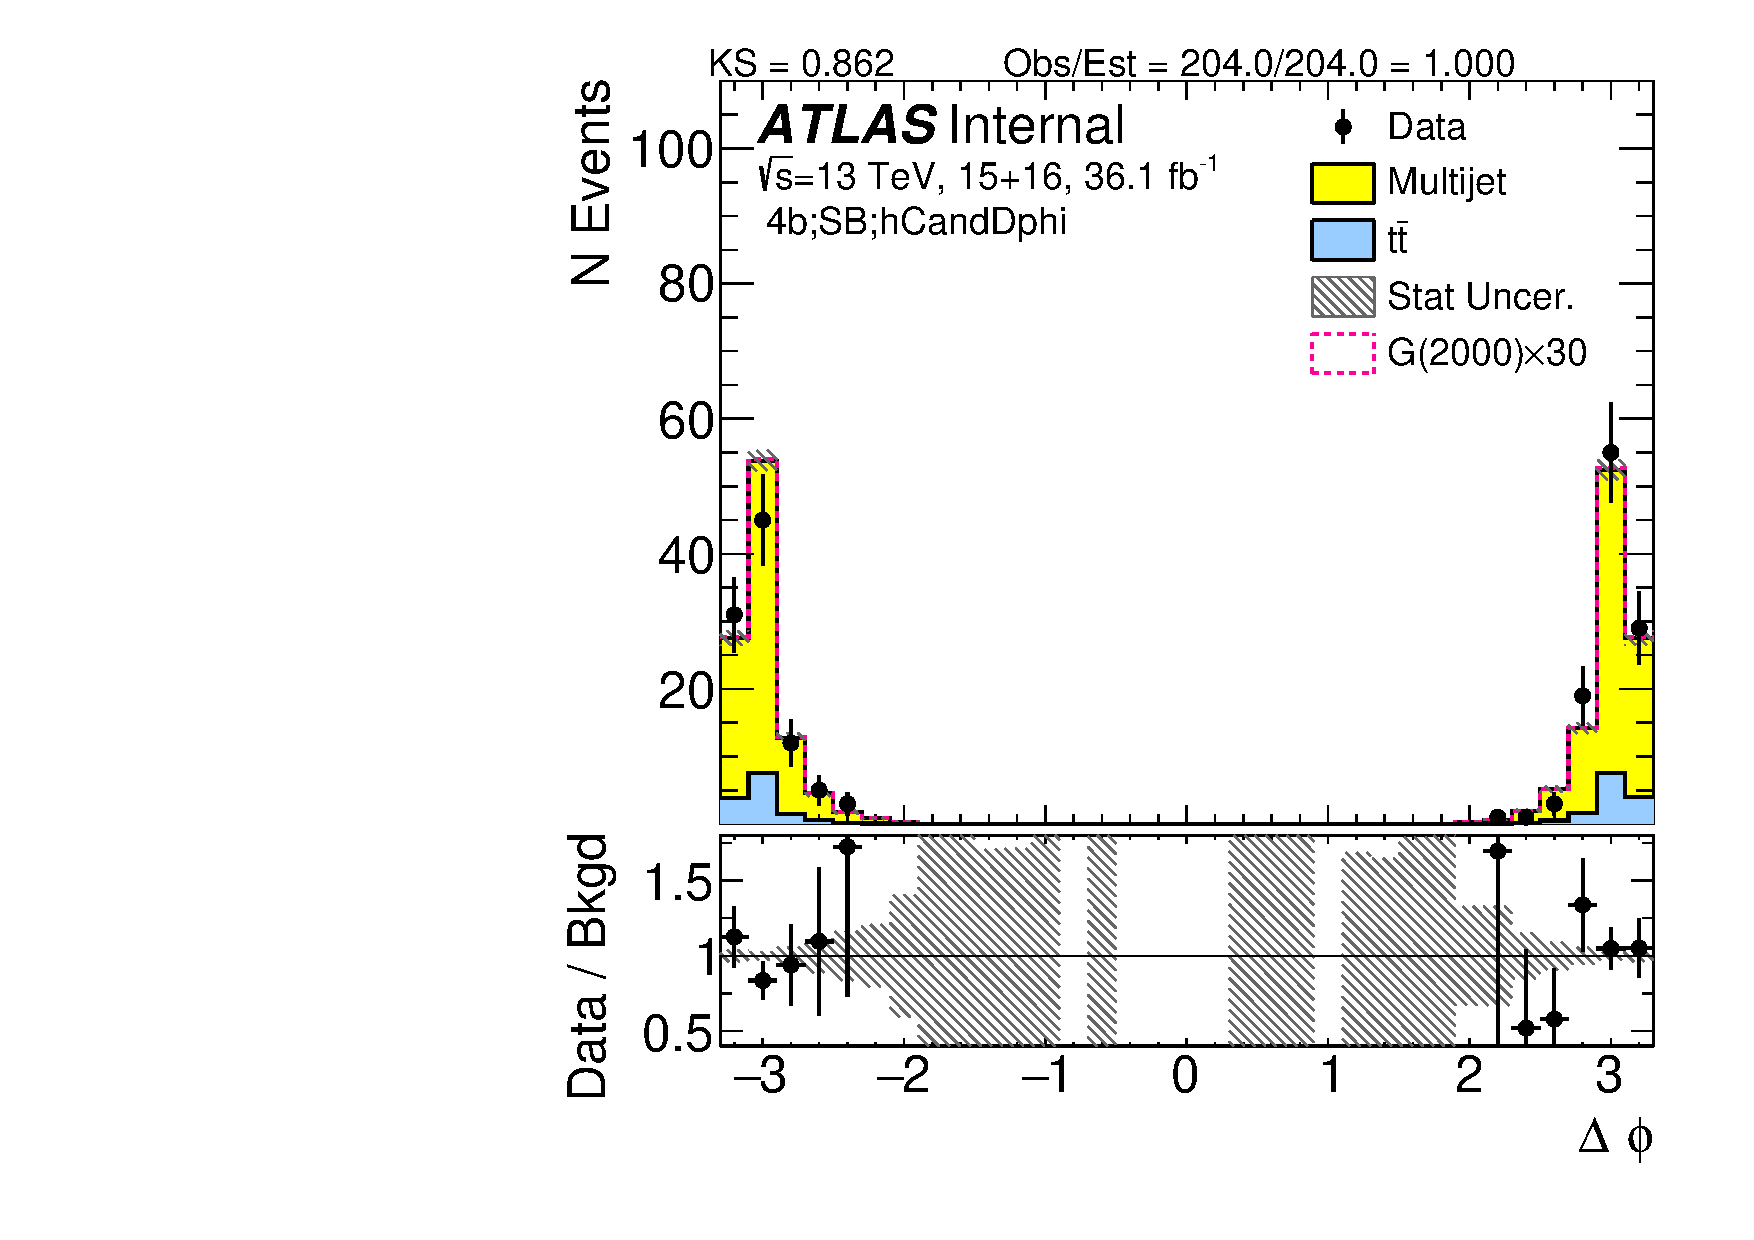
\includegraphics[width=0.32\textwidth,angle=-90]{figures/boosted/Sideband/b77_FourTag_Sideband_hCandDphi.pdf}
  \caption{Kinematics (invariant mass, $\Delta R$, $\Delta \eta$ and $\Delta \phi$) of two large-\R jets in data and prediction in the sideband region after requiring 4 $b$-tags. }
  \label{fig:boosted-4b-sideband-ak10-system}
\end{center}
\end{figure*}

\clearpage

\begin{figure*}[htbp!]
\begin{center}
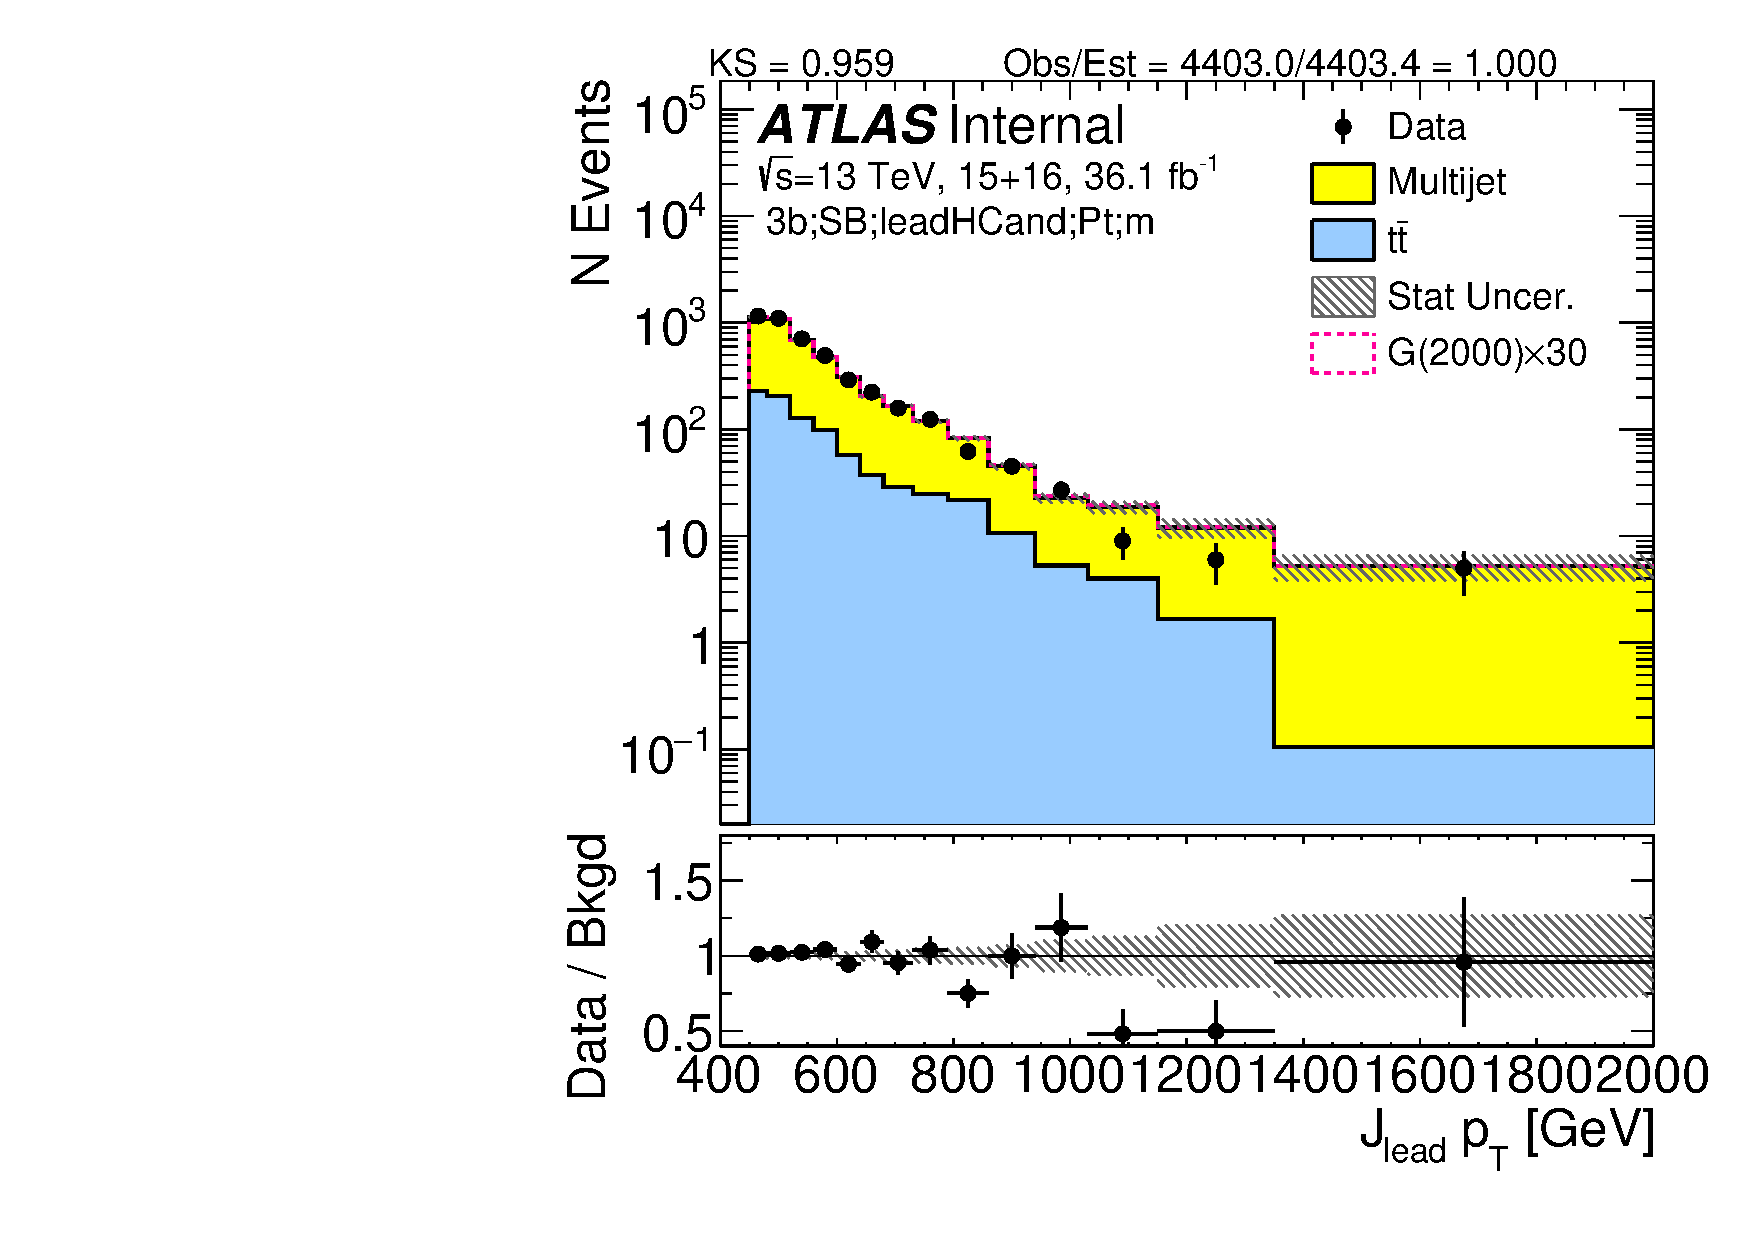
\includegraphics[width=0.32\textwidth,angle=-90]{figures/boosted/Sideband/b77_ThreeTag_Sideband_leadHCand_Pt_m_1.pdf}
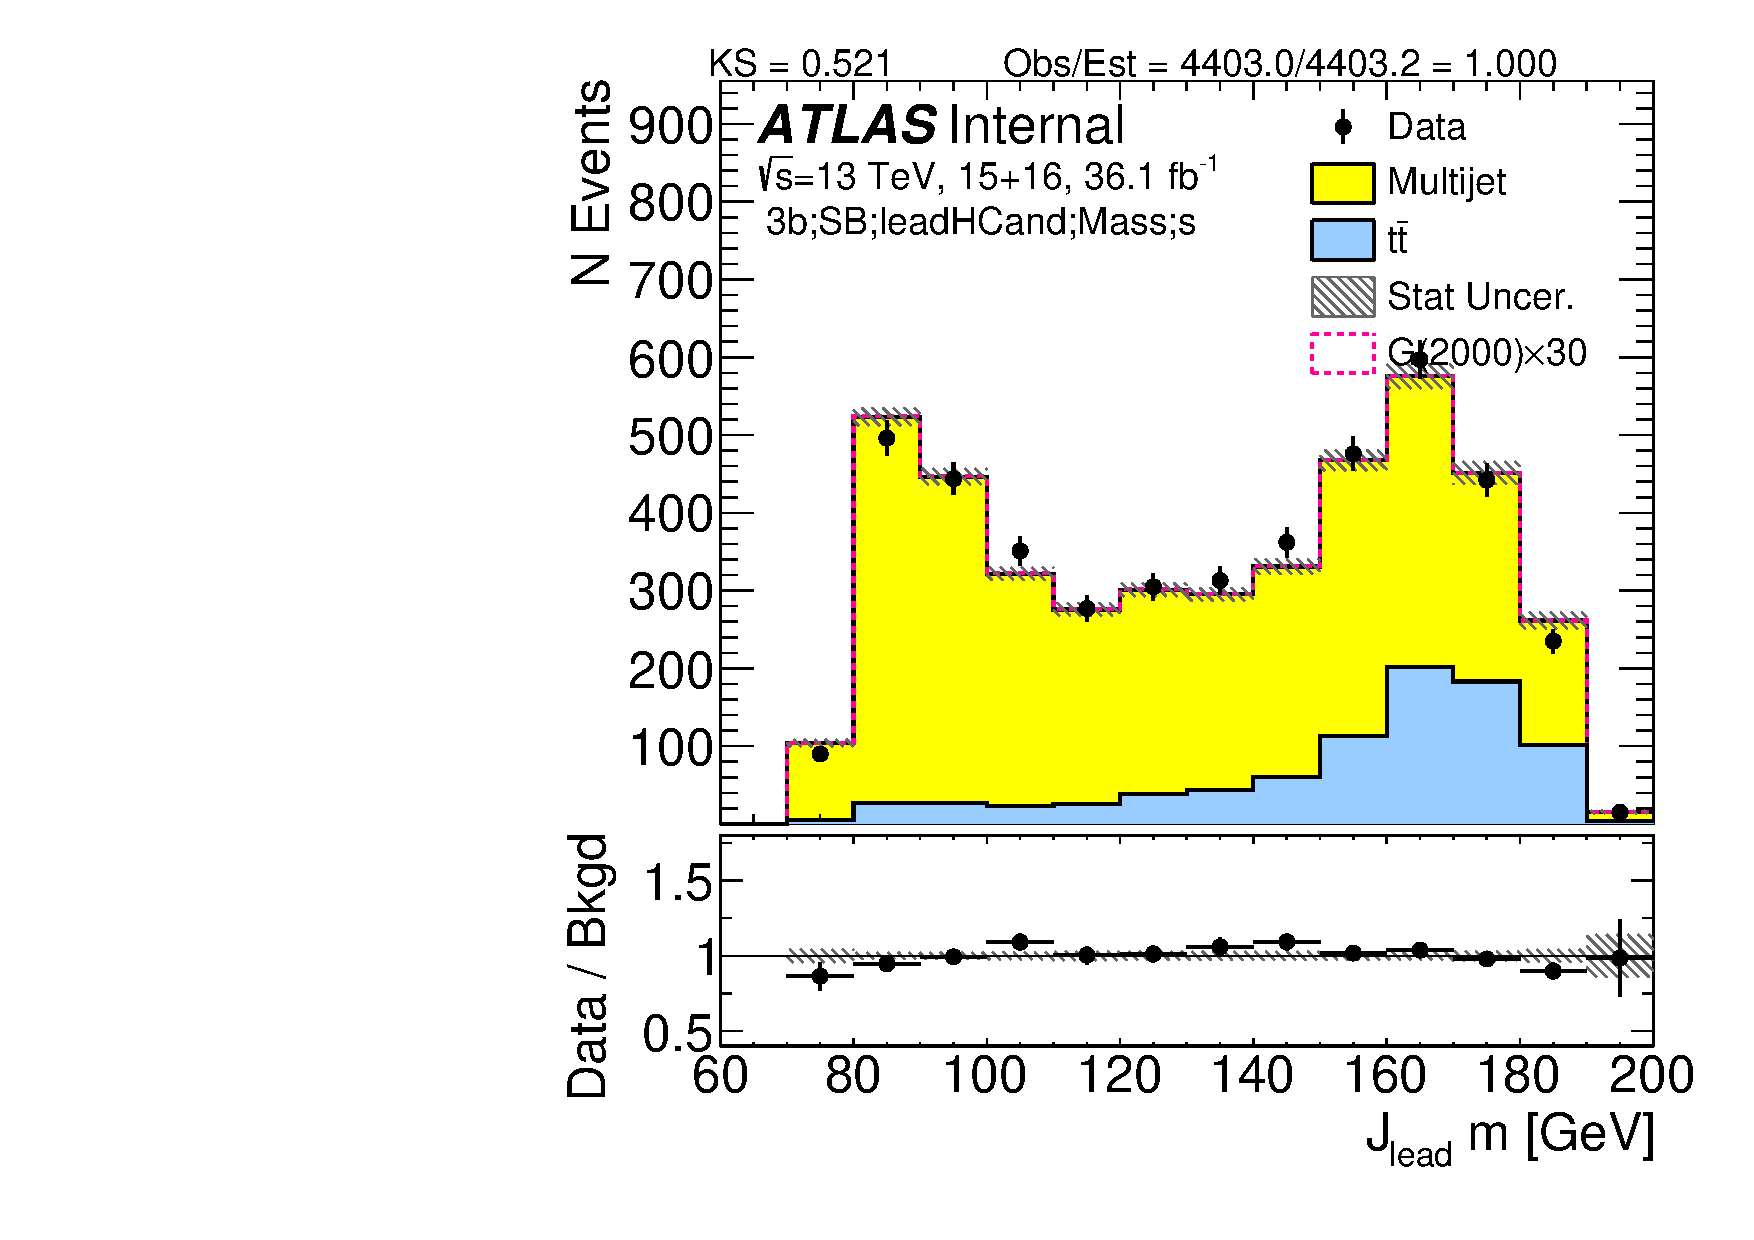
\includegraphics[width=0.32\textwidth,angle=-90]{figures/boosted/Sideband/b77_ThreeTag_Sideband_leadHCand_Mass_s.pdf}\\
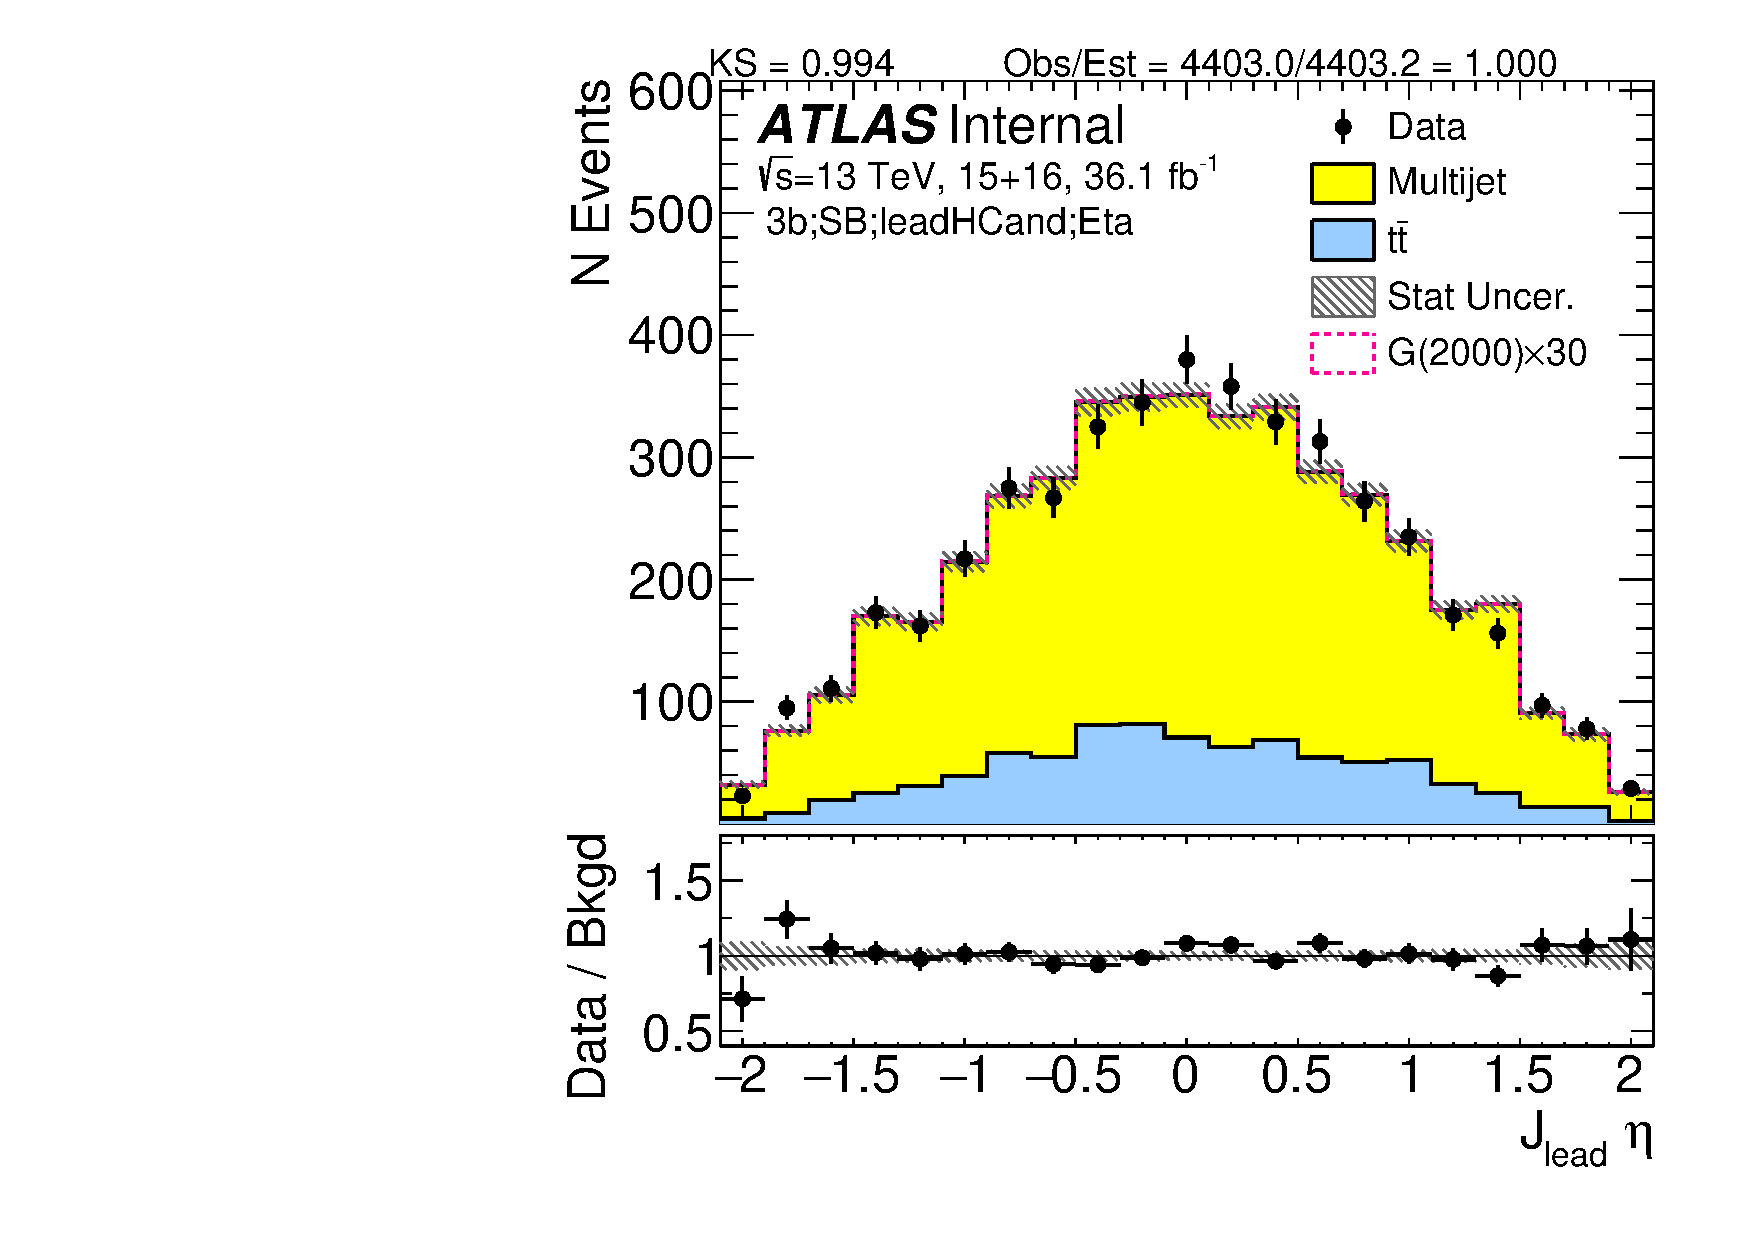
\includegraphics[width=0.32\textwidth,angle=-90]{figures/boosted/Sideband/b77_ThreeTag_Sideband_leadHCand_Eta.pdf}
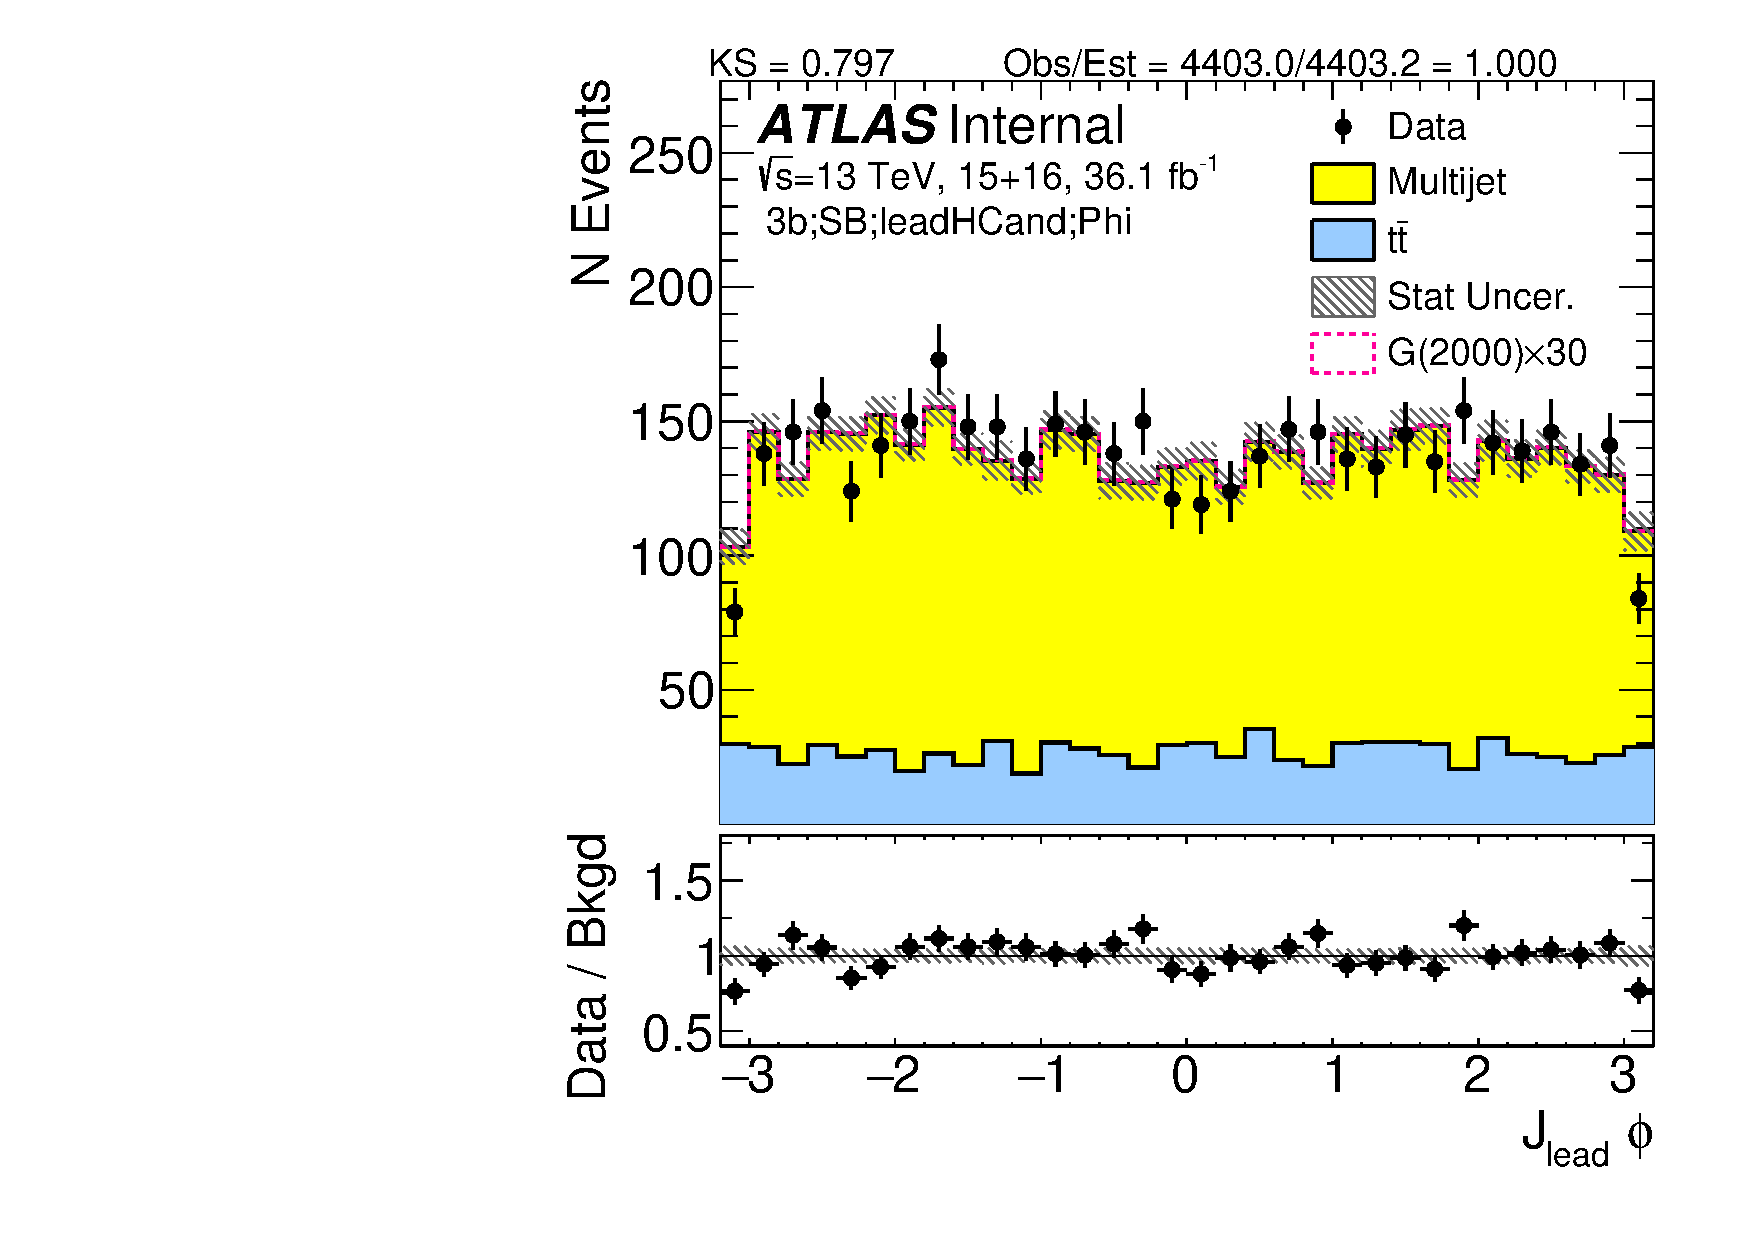
\includegraphics[width=0.32\textwidth,angle=-90]{figures/boosted/Sideband/b77_ThreeTag_Sideband_leadHCand_Phi.pdf}
  \caption{Kinematics (\pt~, mass, $\eta$, $\phi$) of the lead large-\R jet in data and prediction in the sideband region after requiring 3 $b$-tags.}
  \label{fig:boosted-3b-sideband-ak10-lead}
\end{center}
\end{figure*}

\begin{figure*}[htbp!]
\begin{center}
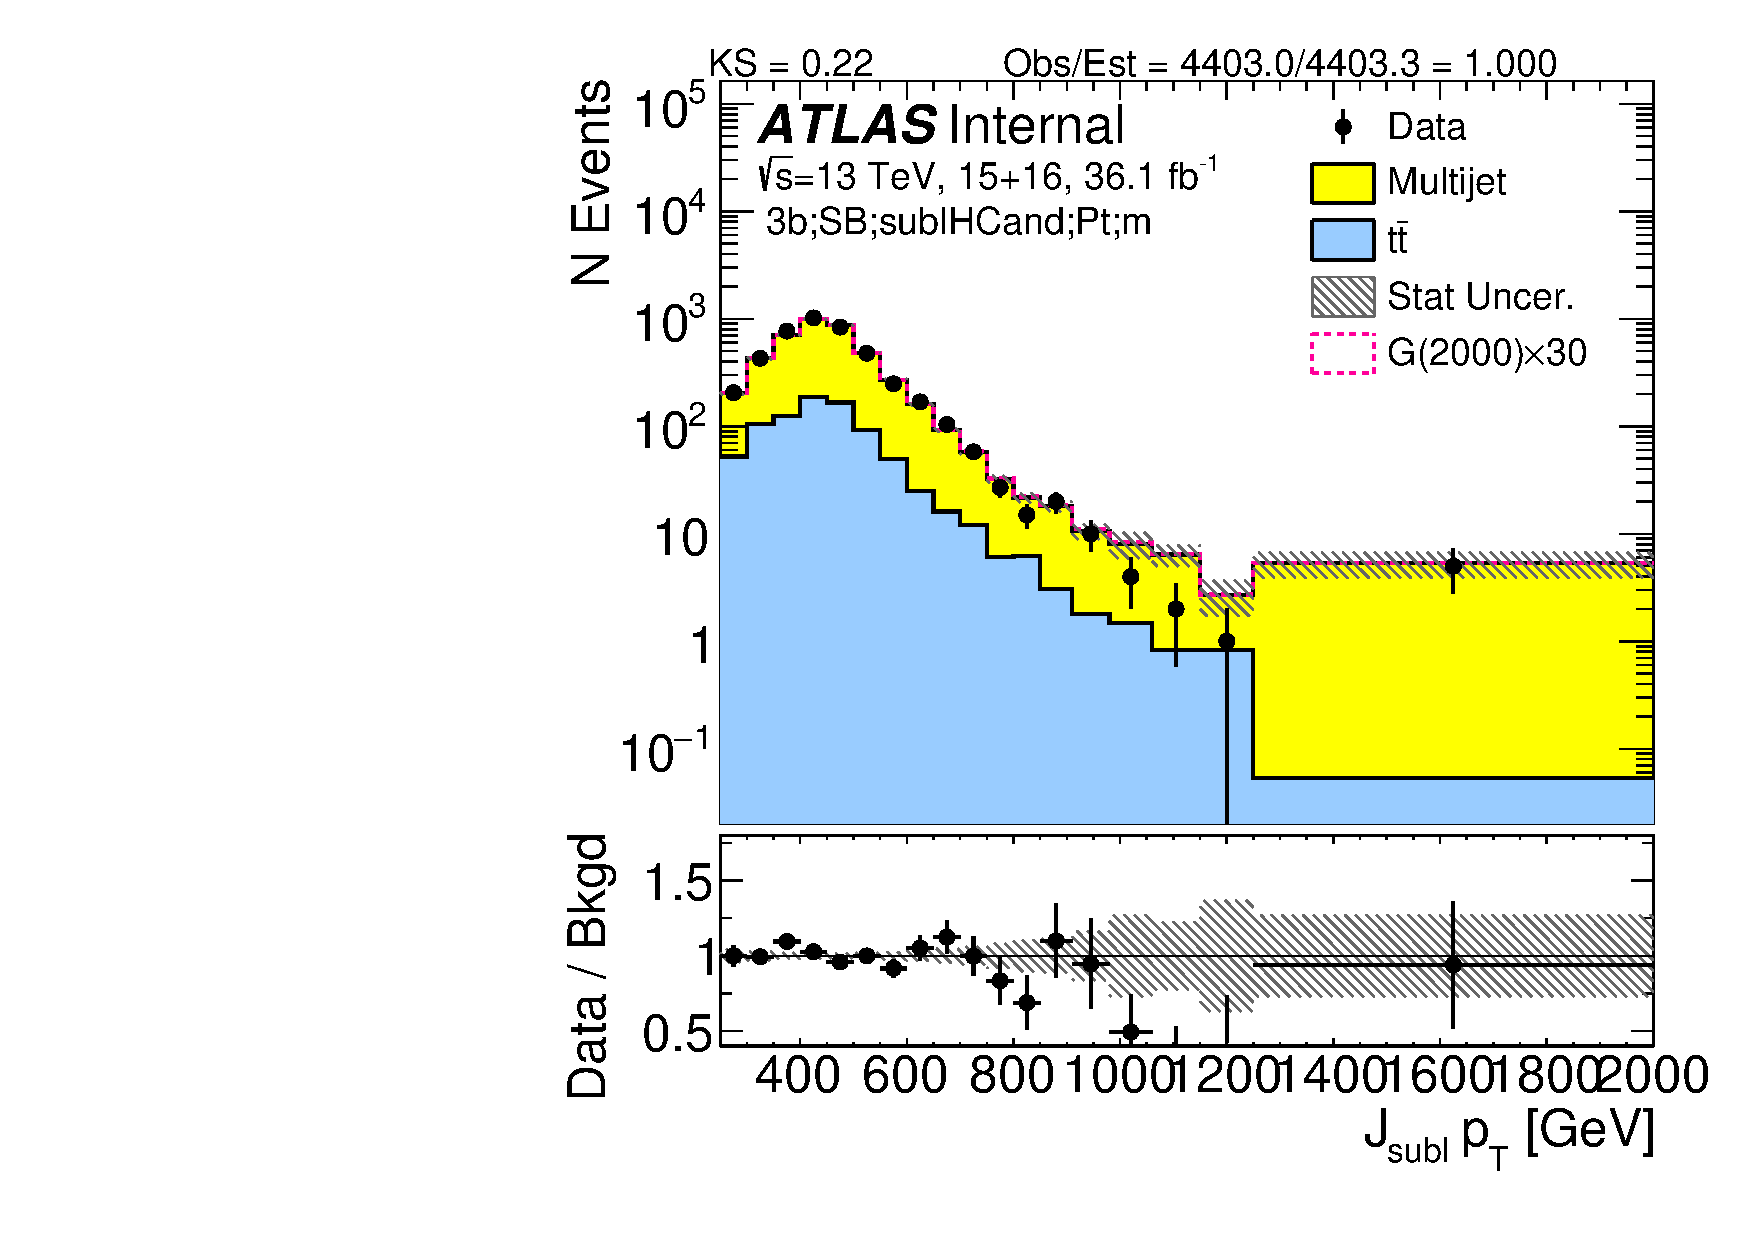
\includegraphics[width=0.32\textwidth,angle=-90]{figures/boosted/Sideband/b77_ThreeTag_Sideband_sublHCand_Pt_m_1.pdf}
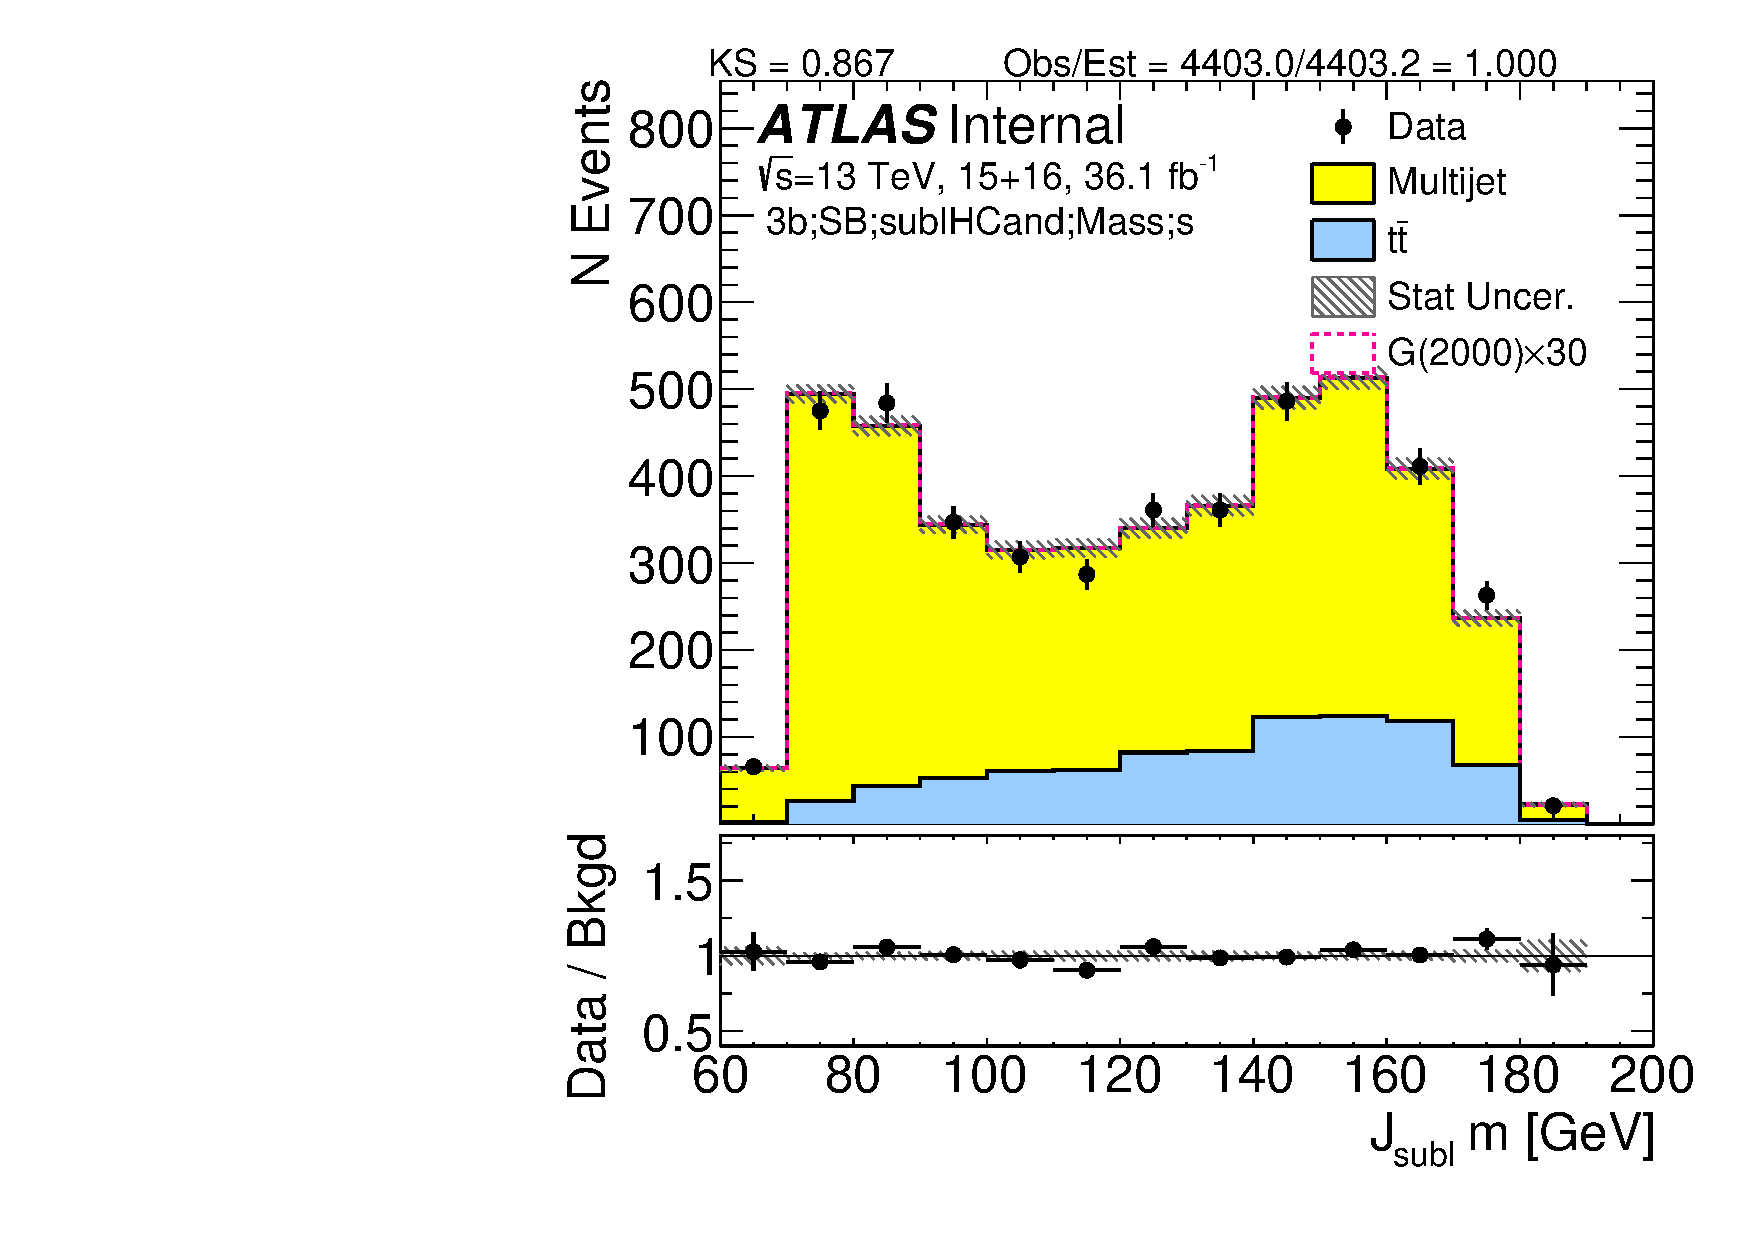
\includegraphics[width=0.32\textwidth,angle=-90]{figures/boosted/Sideband/b77_ThreeTag_Sideband_sublHCand_Mass_s.pdf}\\
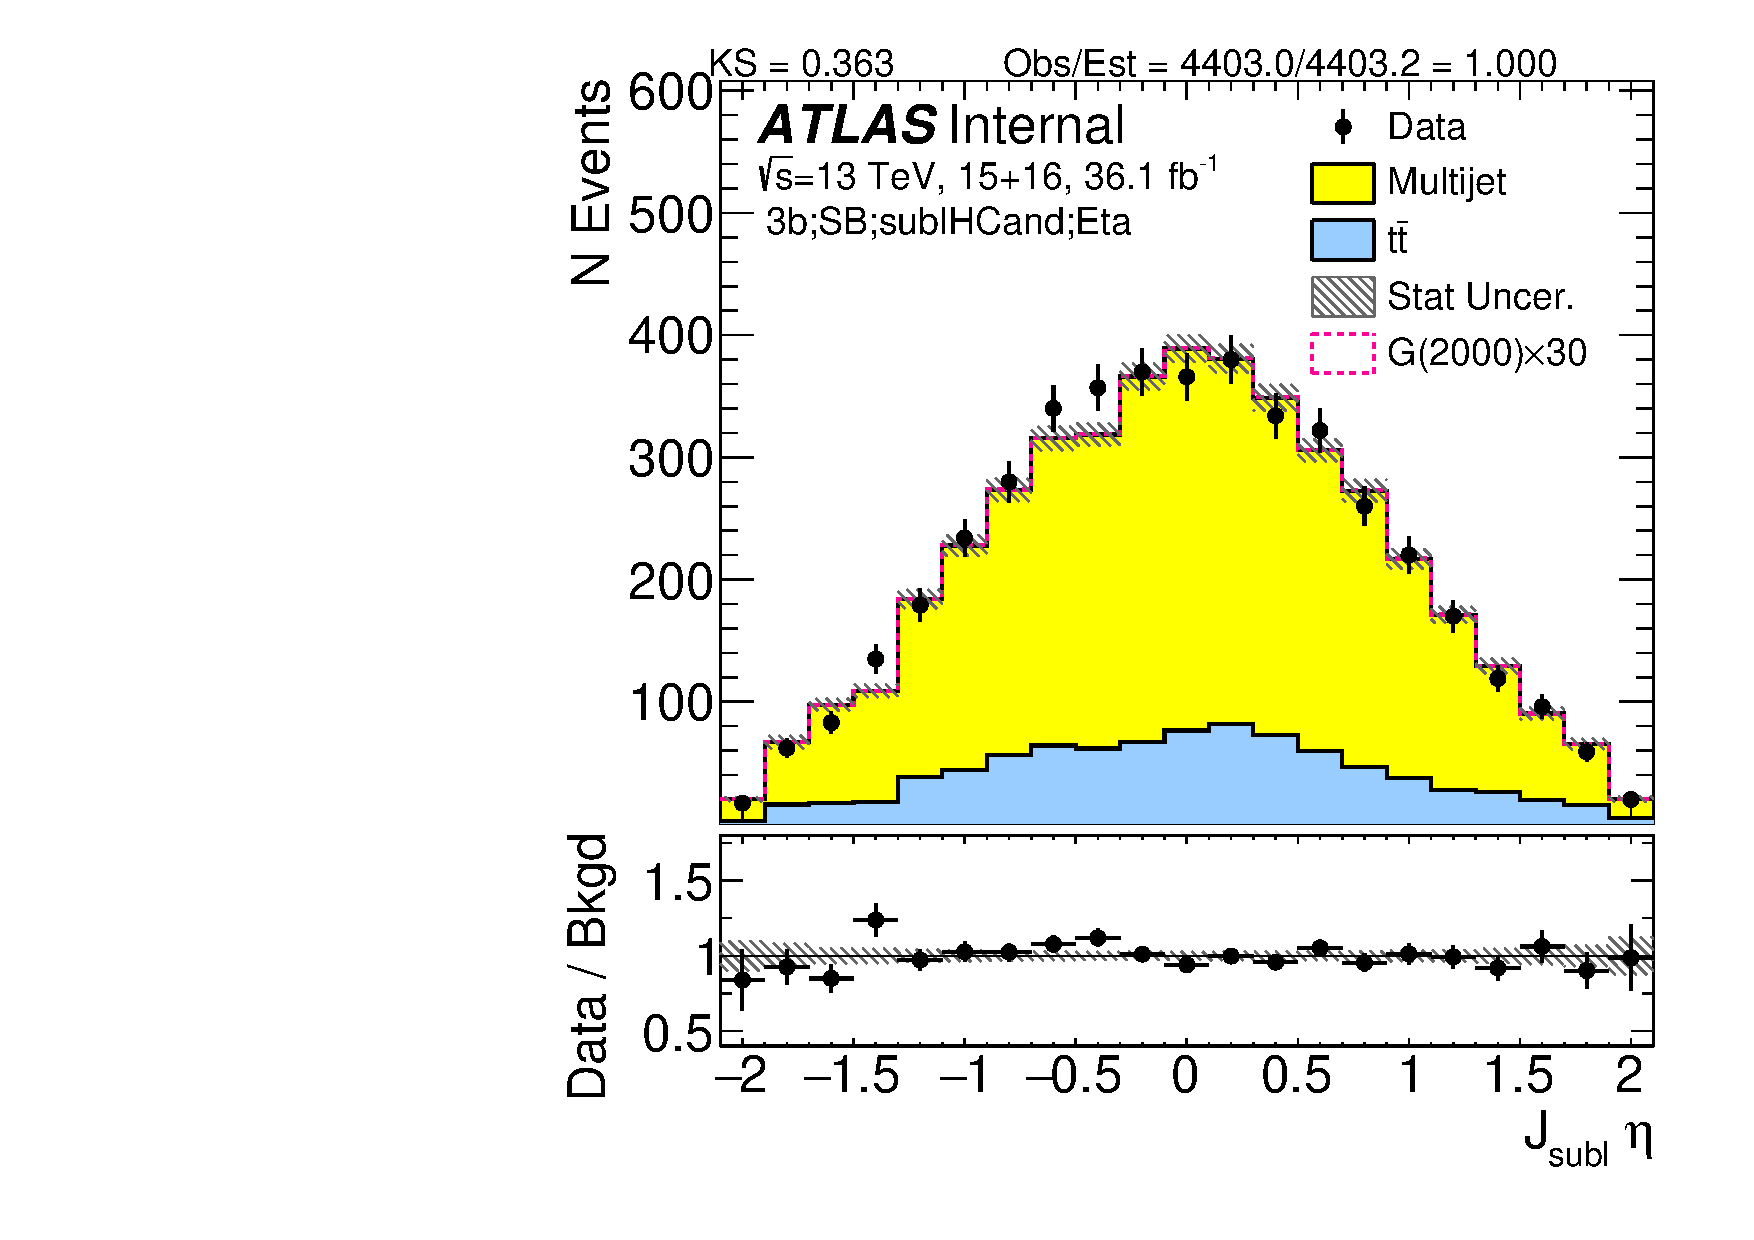
\includegraphics[width=0.32\textwidth,angle=-90]{figures/boosted/Sideband/b77_ThreeTag_Sideband_sublHCand_Eta.pdf}
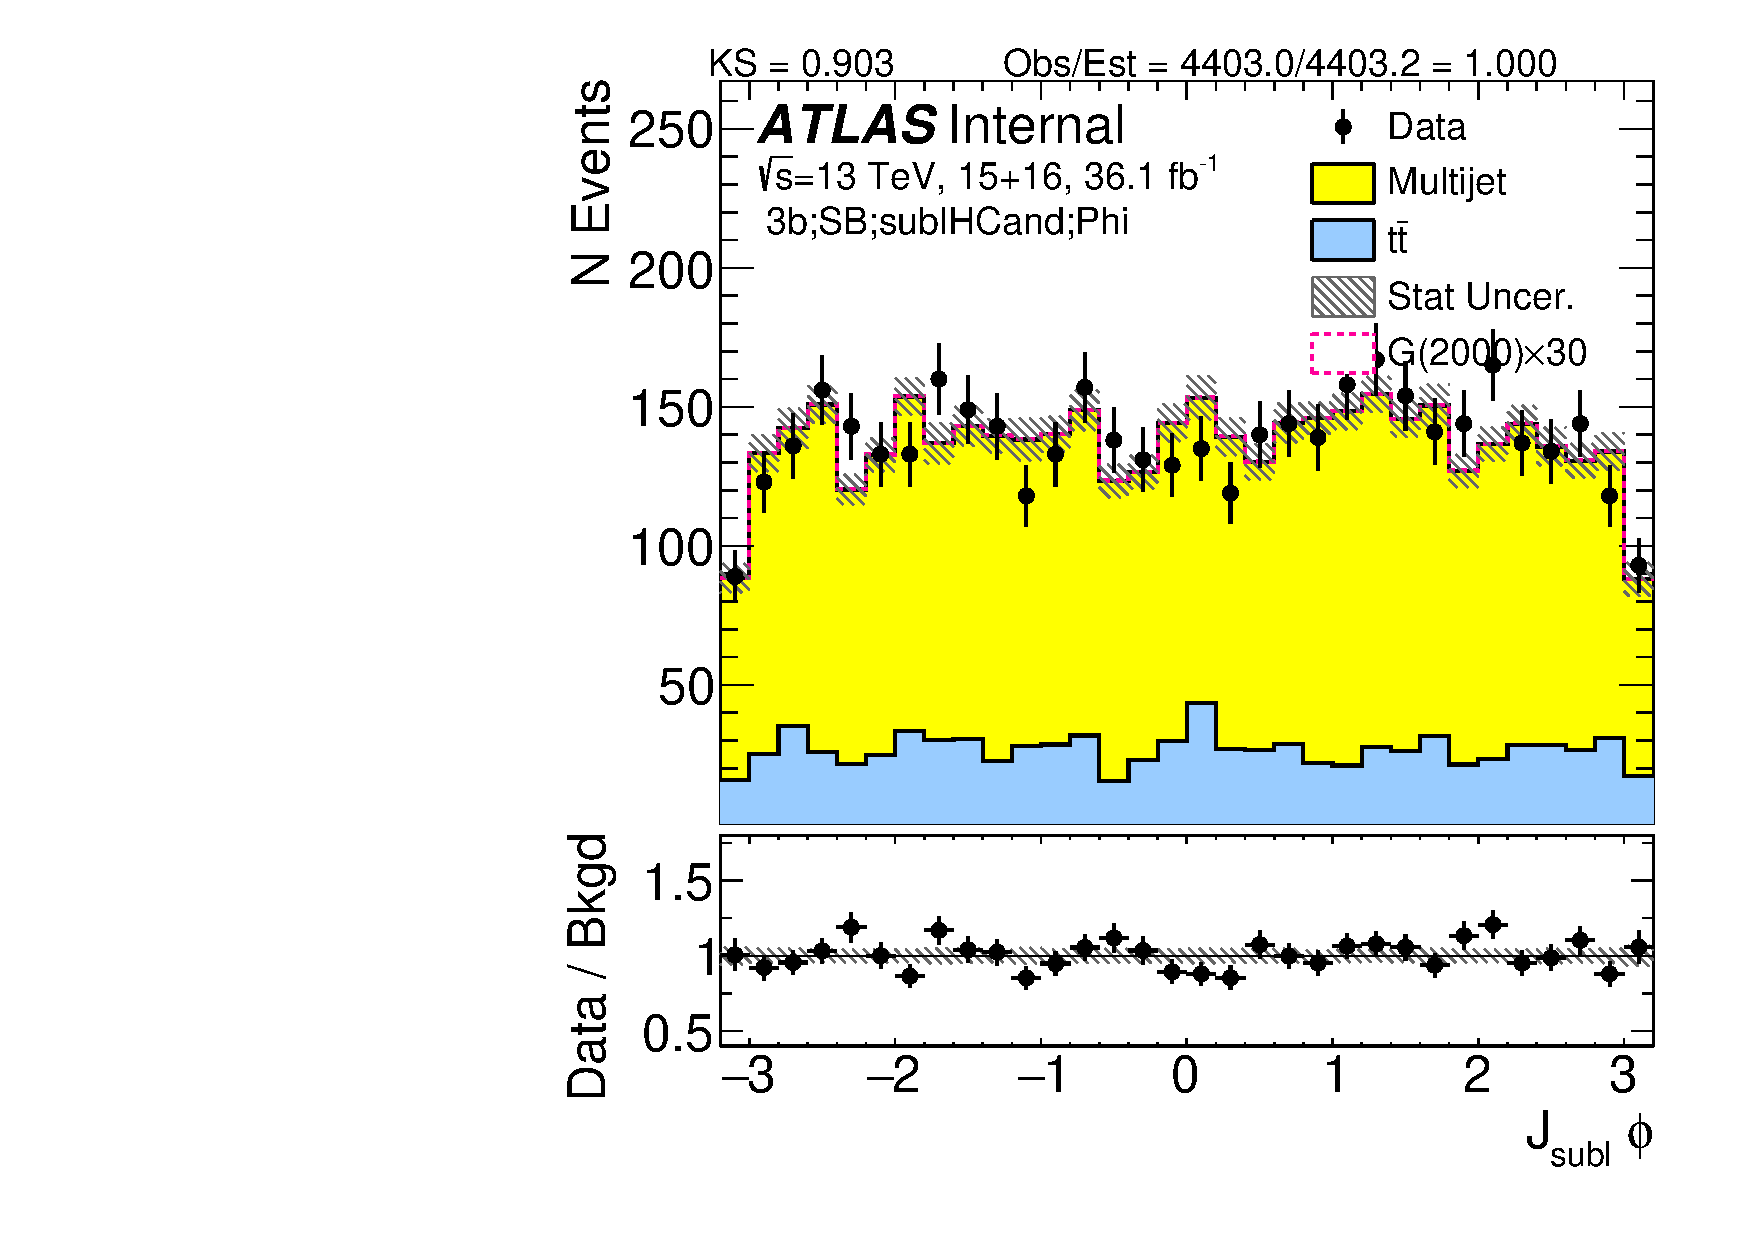
\includegraphics[width=0.32\textwidth,angle=-90]{figures/boosted/Sideband/b77_ThreeTag_Sideband_sublHCand_Phi.pdf}
  \caption{Kinematics (\pt~, mass, $\eta$, $\phi$) of the subleading large-\R jet in data and prediction in the sideband region after requiring 3 $b$-tags.}
  \label{fig:boosted-3b-sideband-ak10-subl}
\end{center}
\end{figure*}

\begin{figure*}[htbp!]
\begin{center}
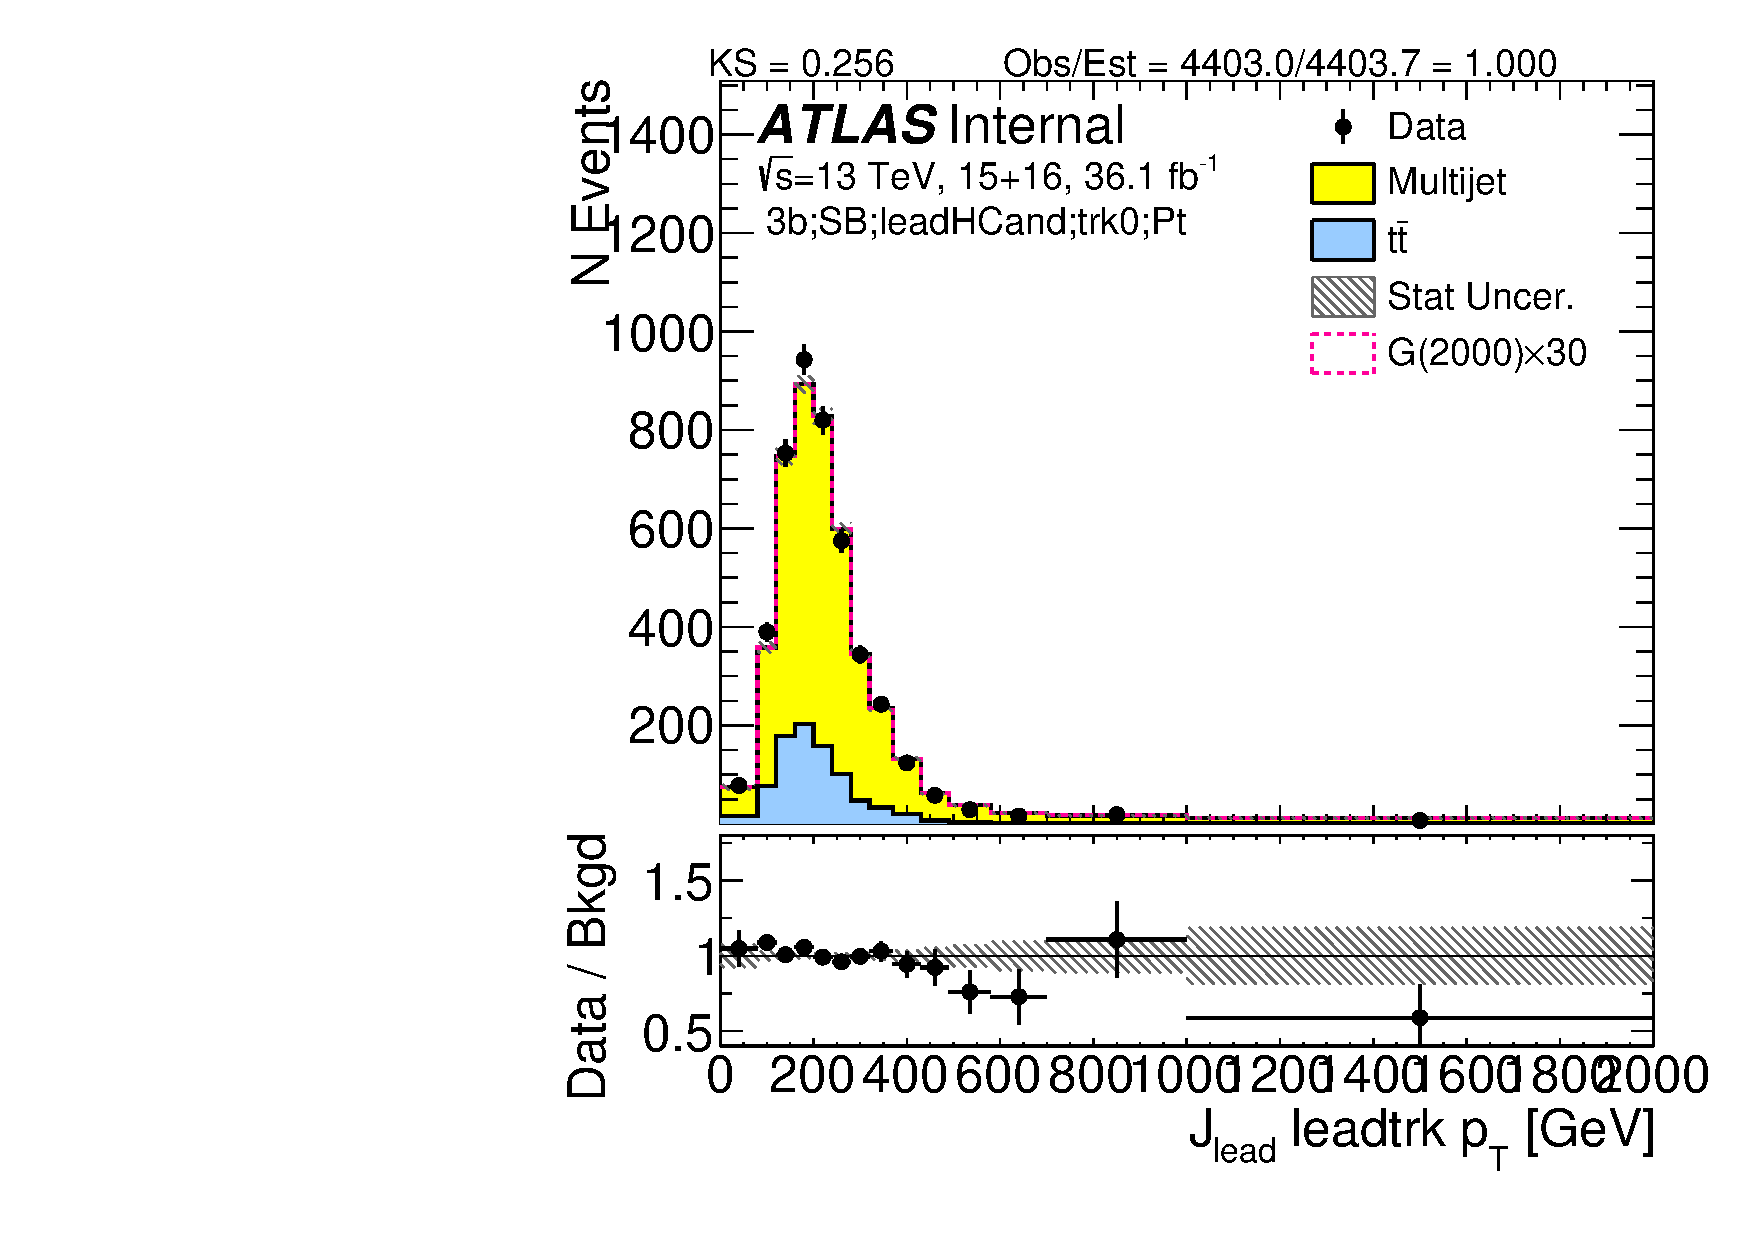
\includegraphics[width=0.32\textwidth,angle=-90]{figures/boosted/Sideband/b77_ThreeTag_Sideband_leadHCand_trk0_Pt.pdf}
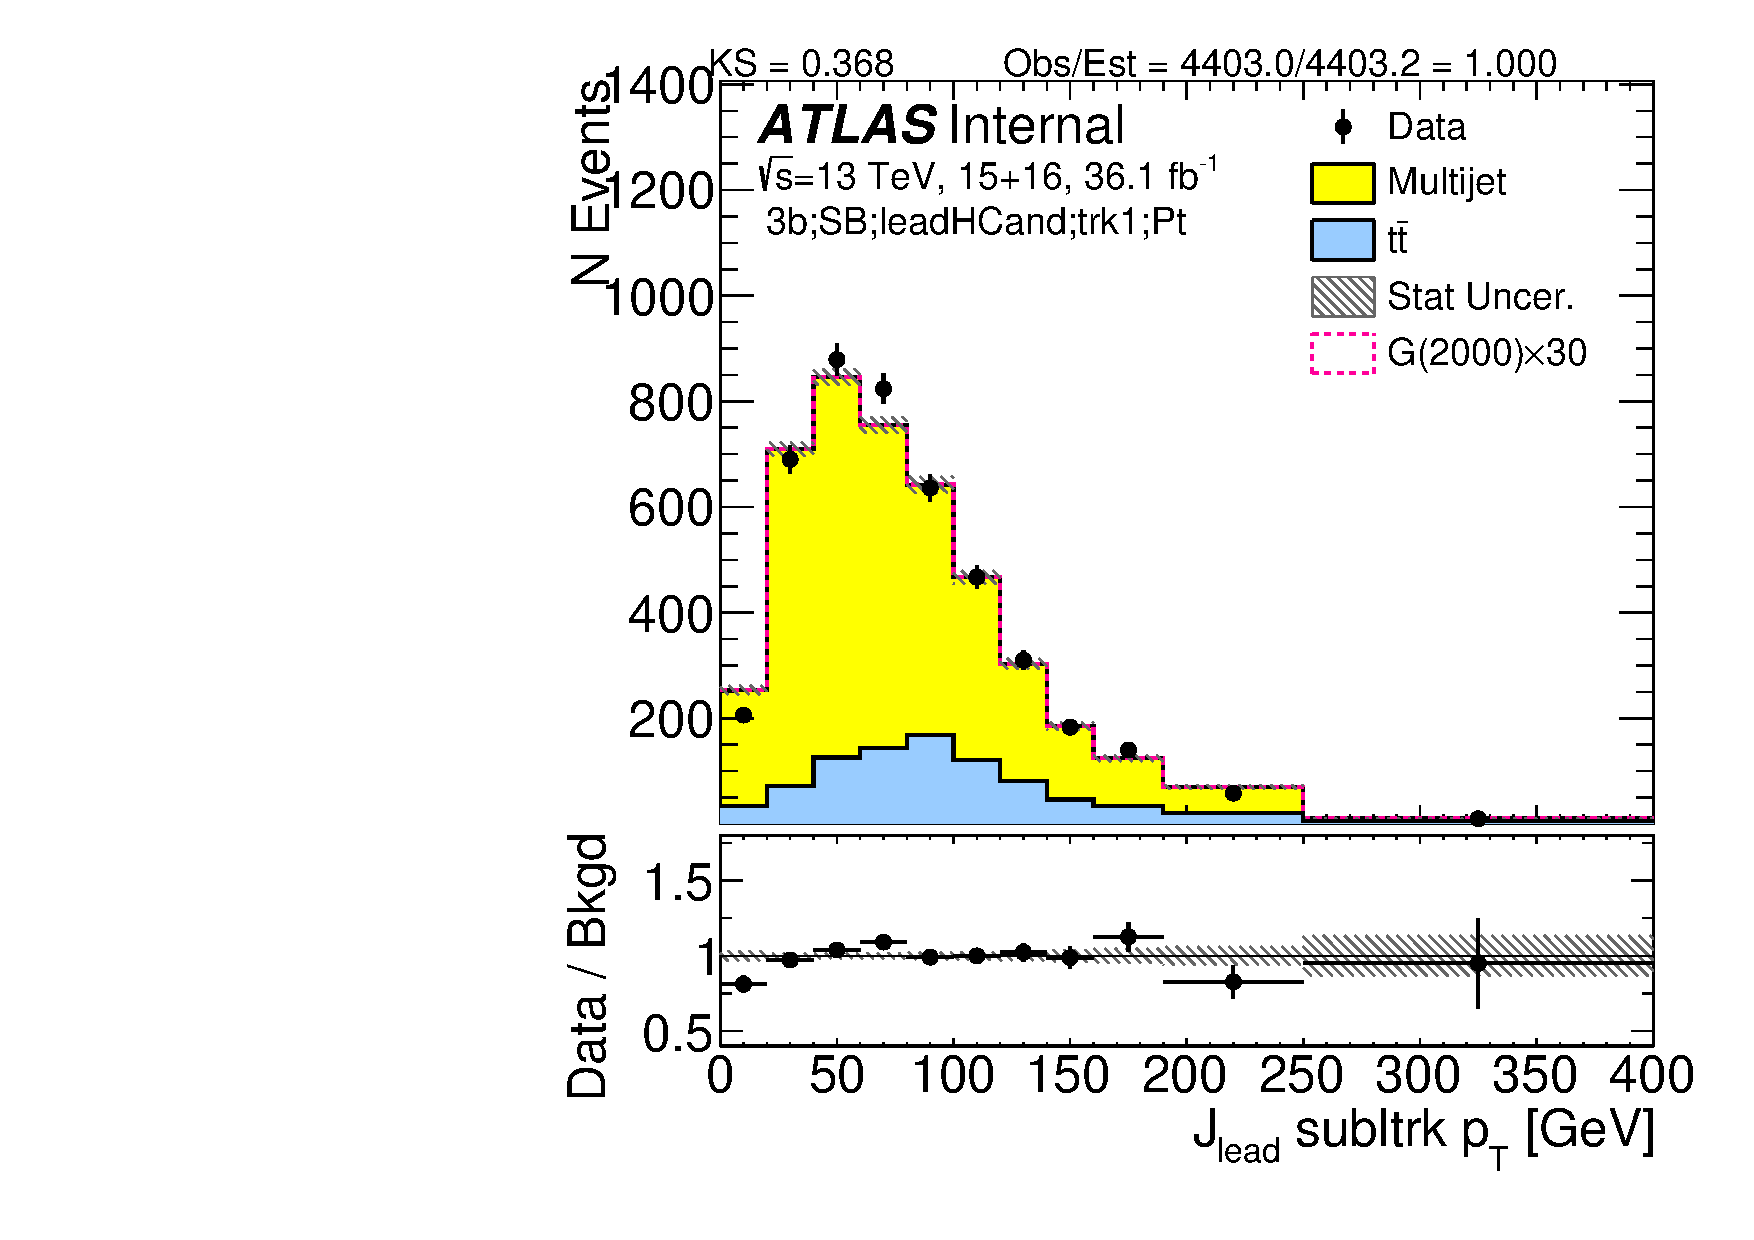
\includegraphics[width=0.32\textwidth,angle=-90]{figures/boosted/Sideband/b77_ThreeTag_Sideband_leadHCand_trk1_Pt.pdf}\\
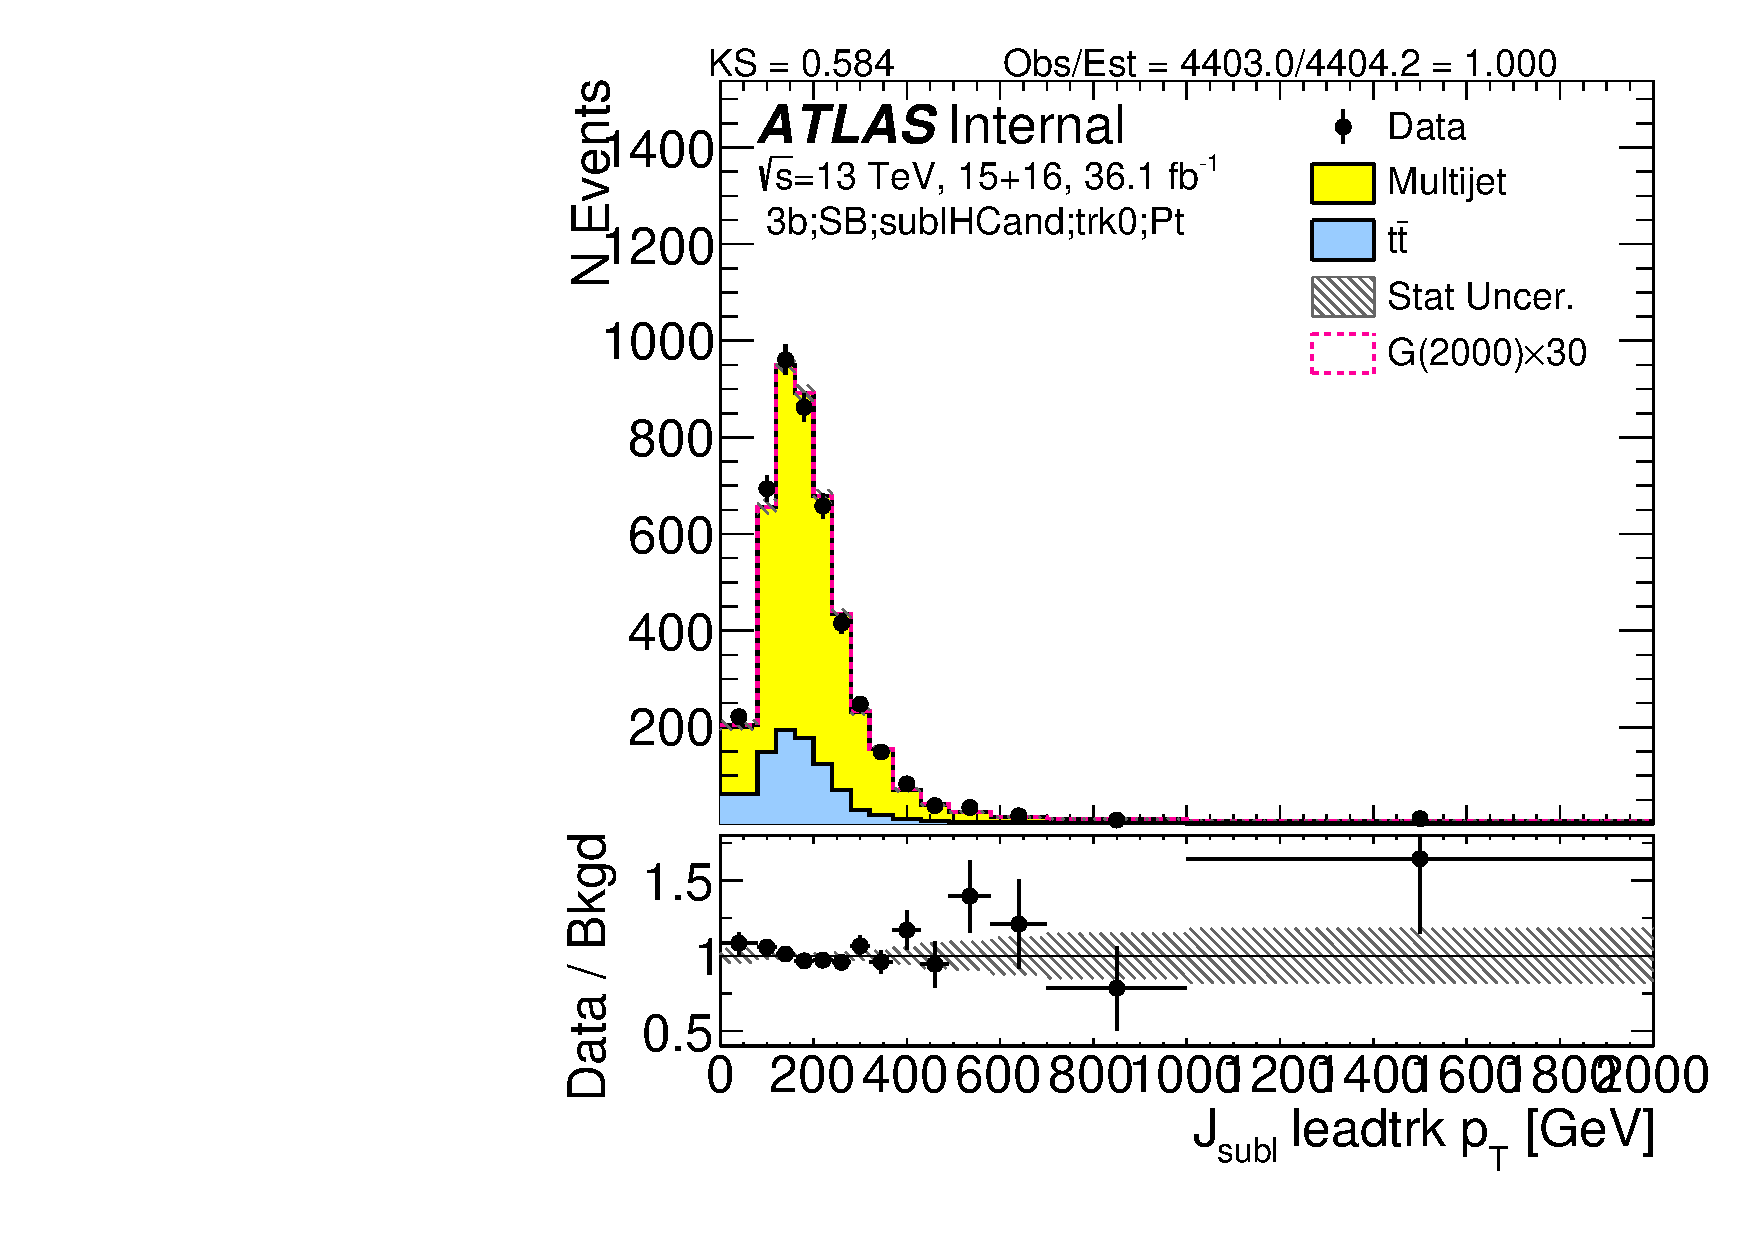
\includegraphics[width=0.32\textwidth,angle=-90]{figures/boosted/Sideband/b77_ThreeTag_Sideband_sublHCand_trk0_Pt.pdf}
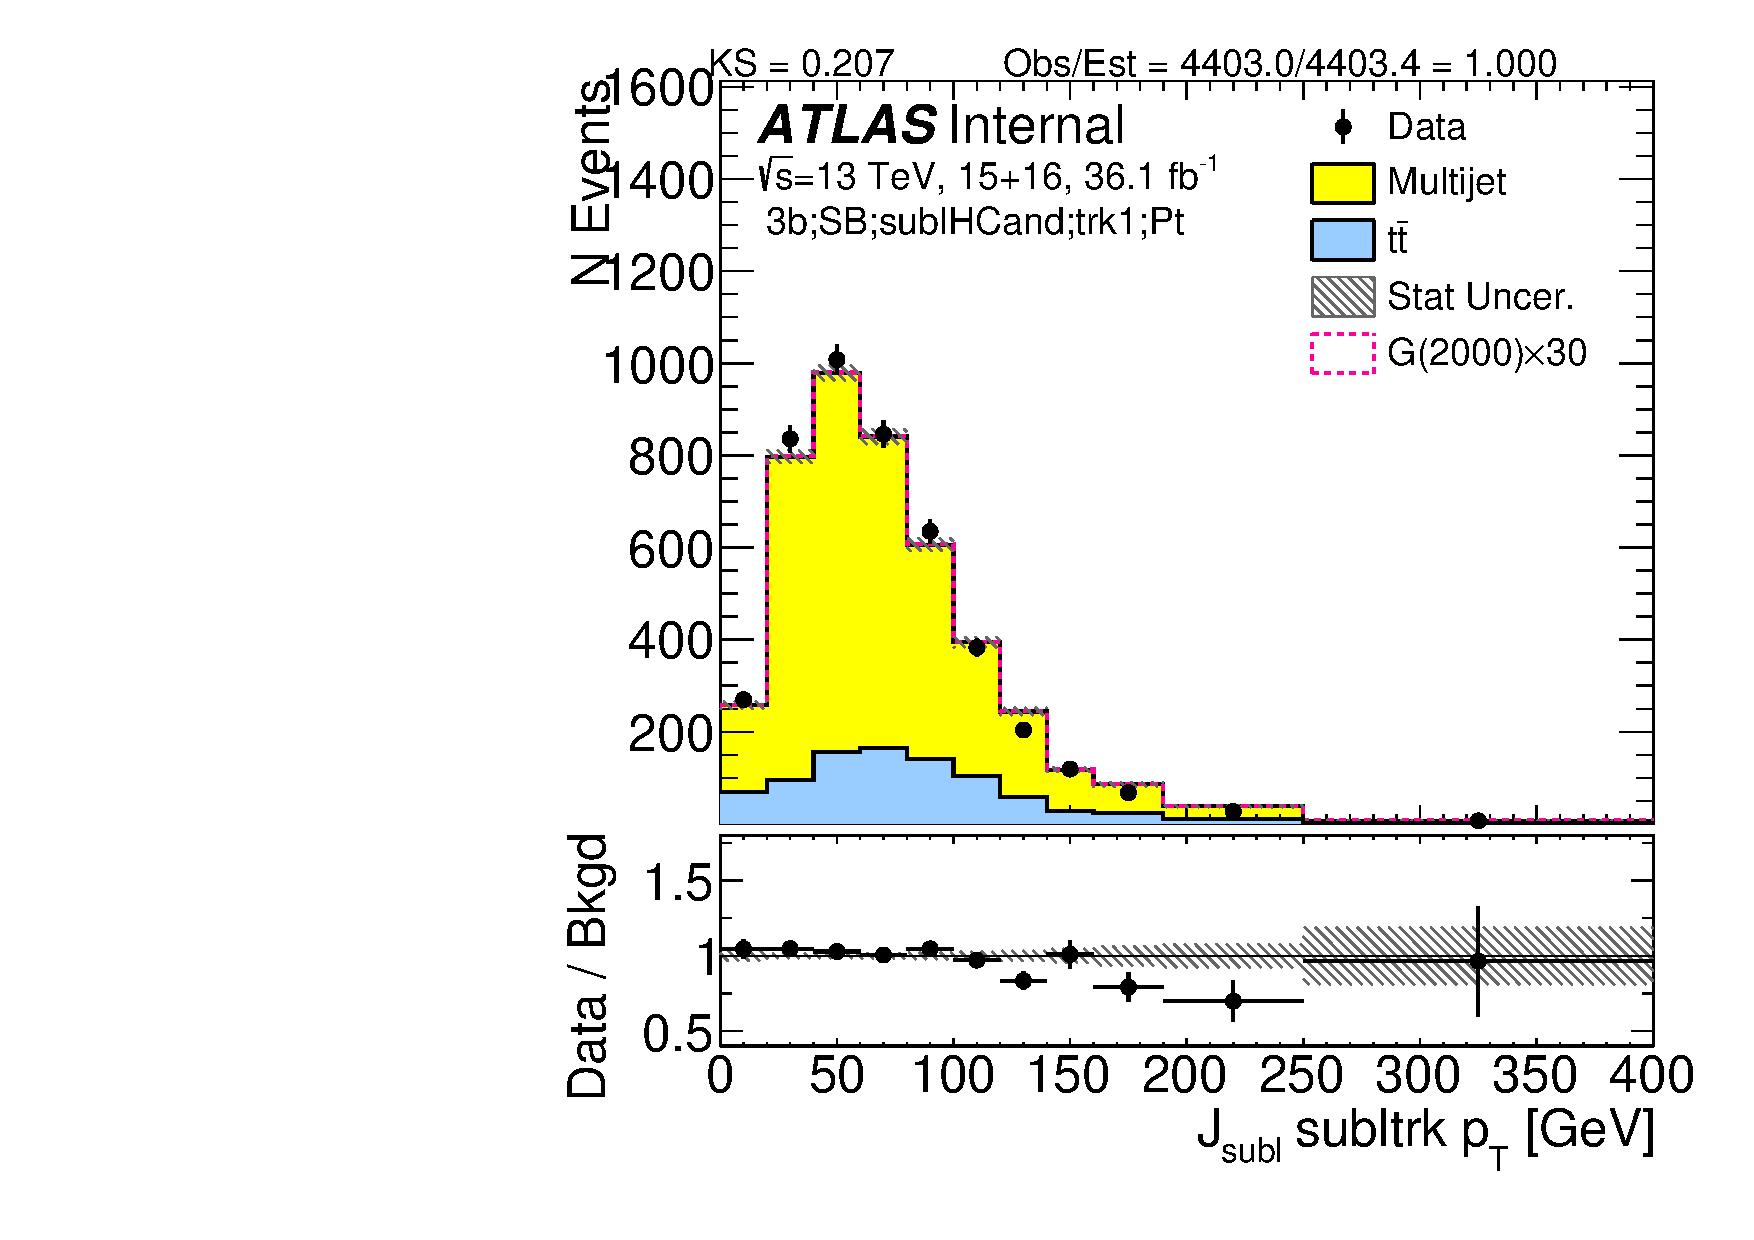
\includegraphics[width=0.32\textwidth,angle=-90]{figures/boosted/Sideband/b77_ThreeTag_Sideband_sublHCand_trk1_Pt.pdf}\\
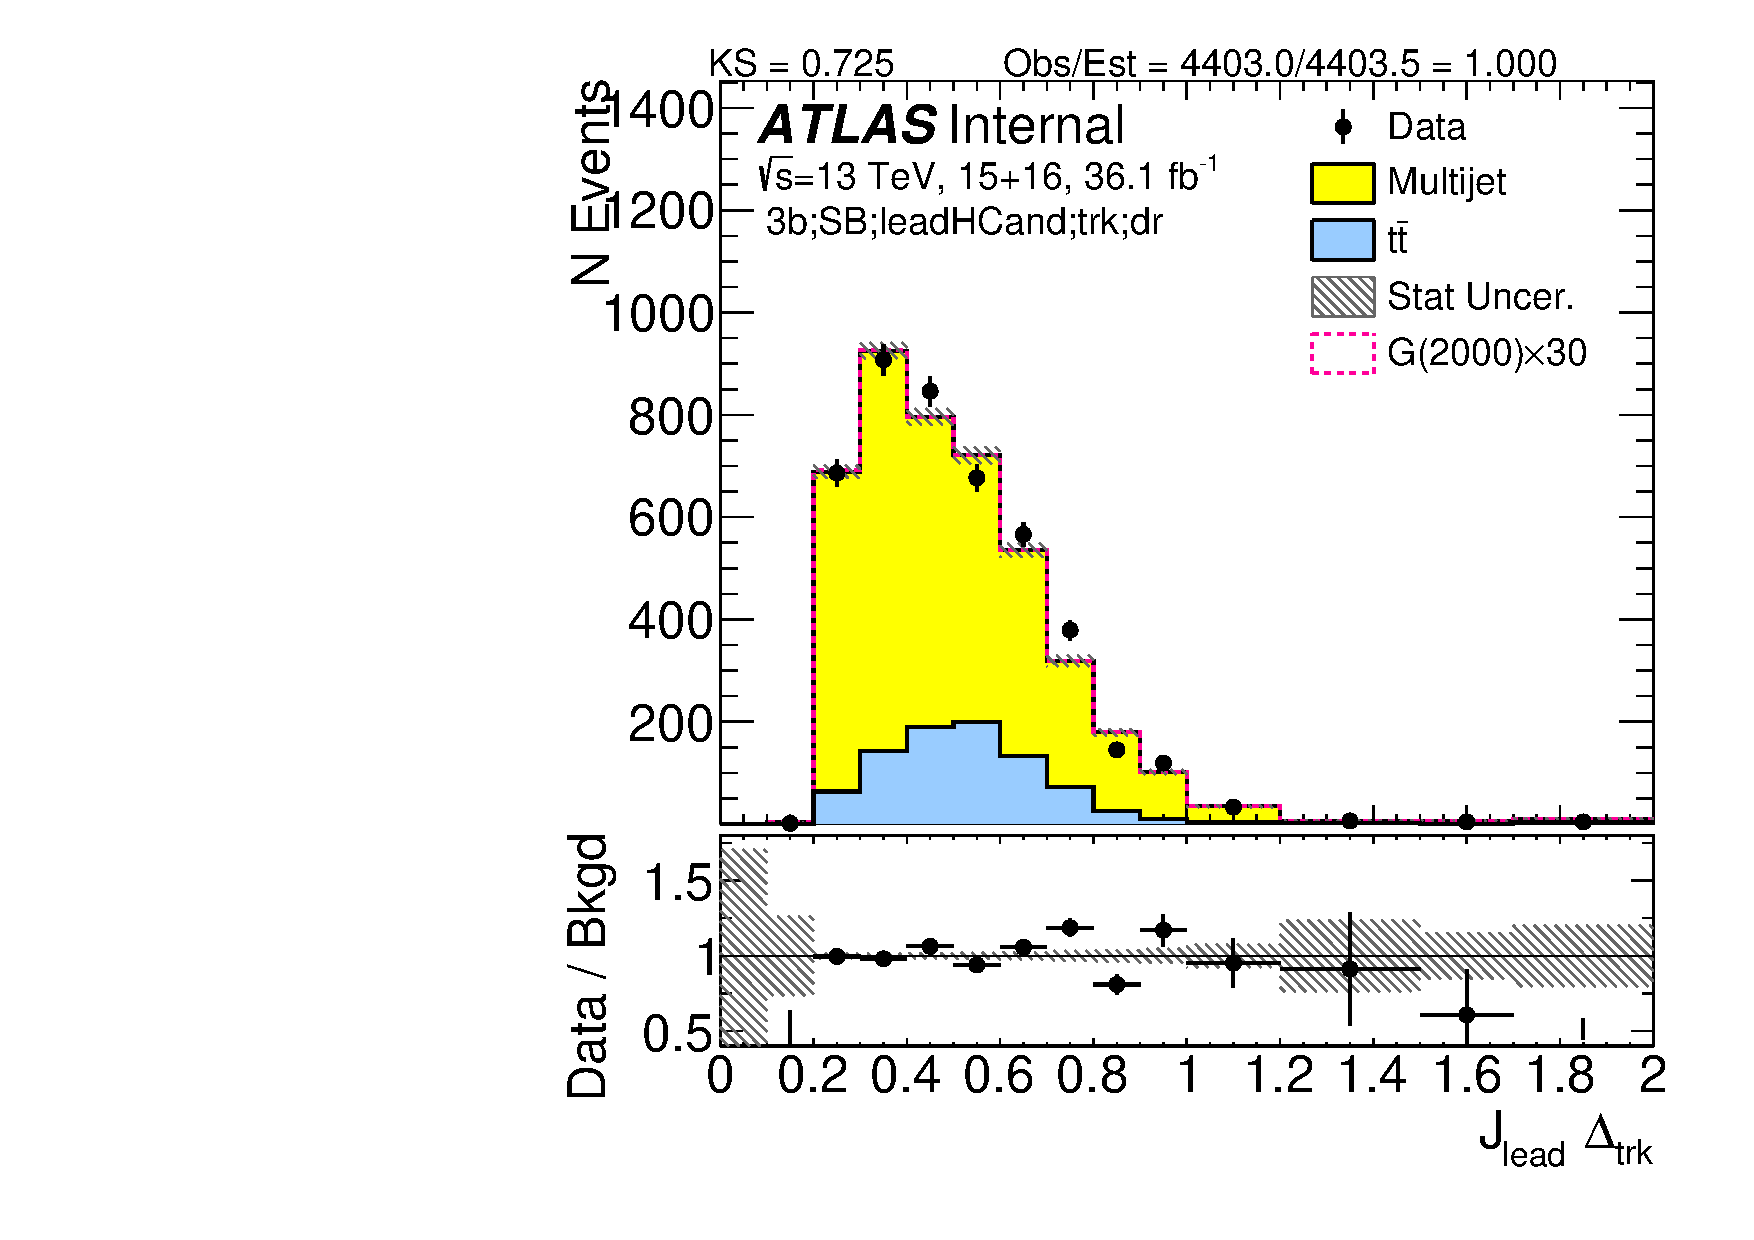
\includegraphics[width=0.32\textwidth,angle=-90]{figures/boosted/Sideband/b77_ThreeTag_Sideband_leadHCand_trk_dr.pdf}
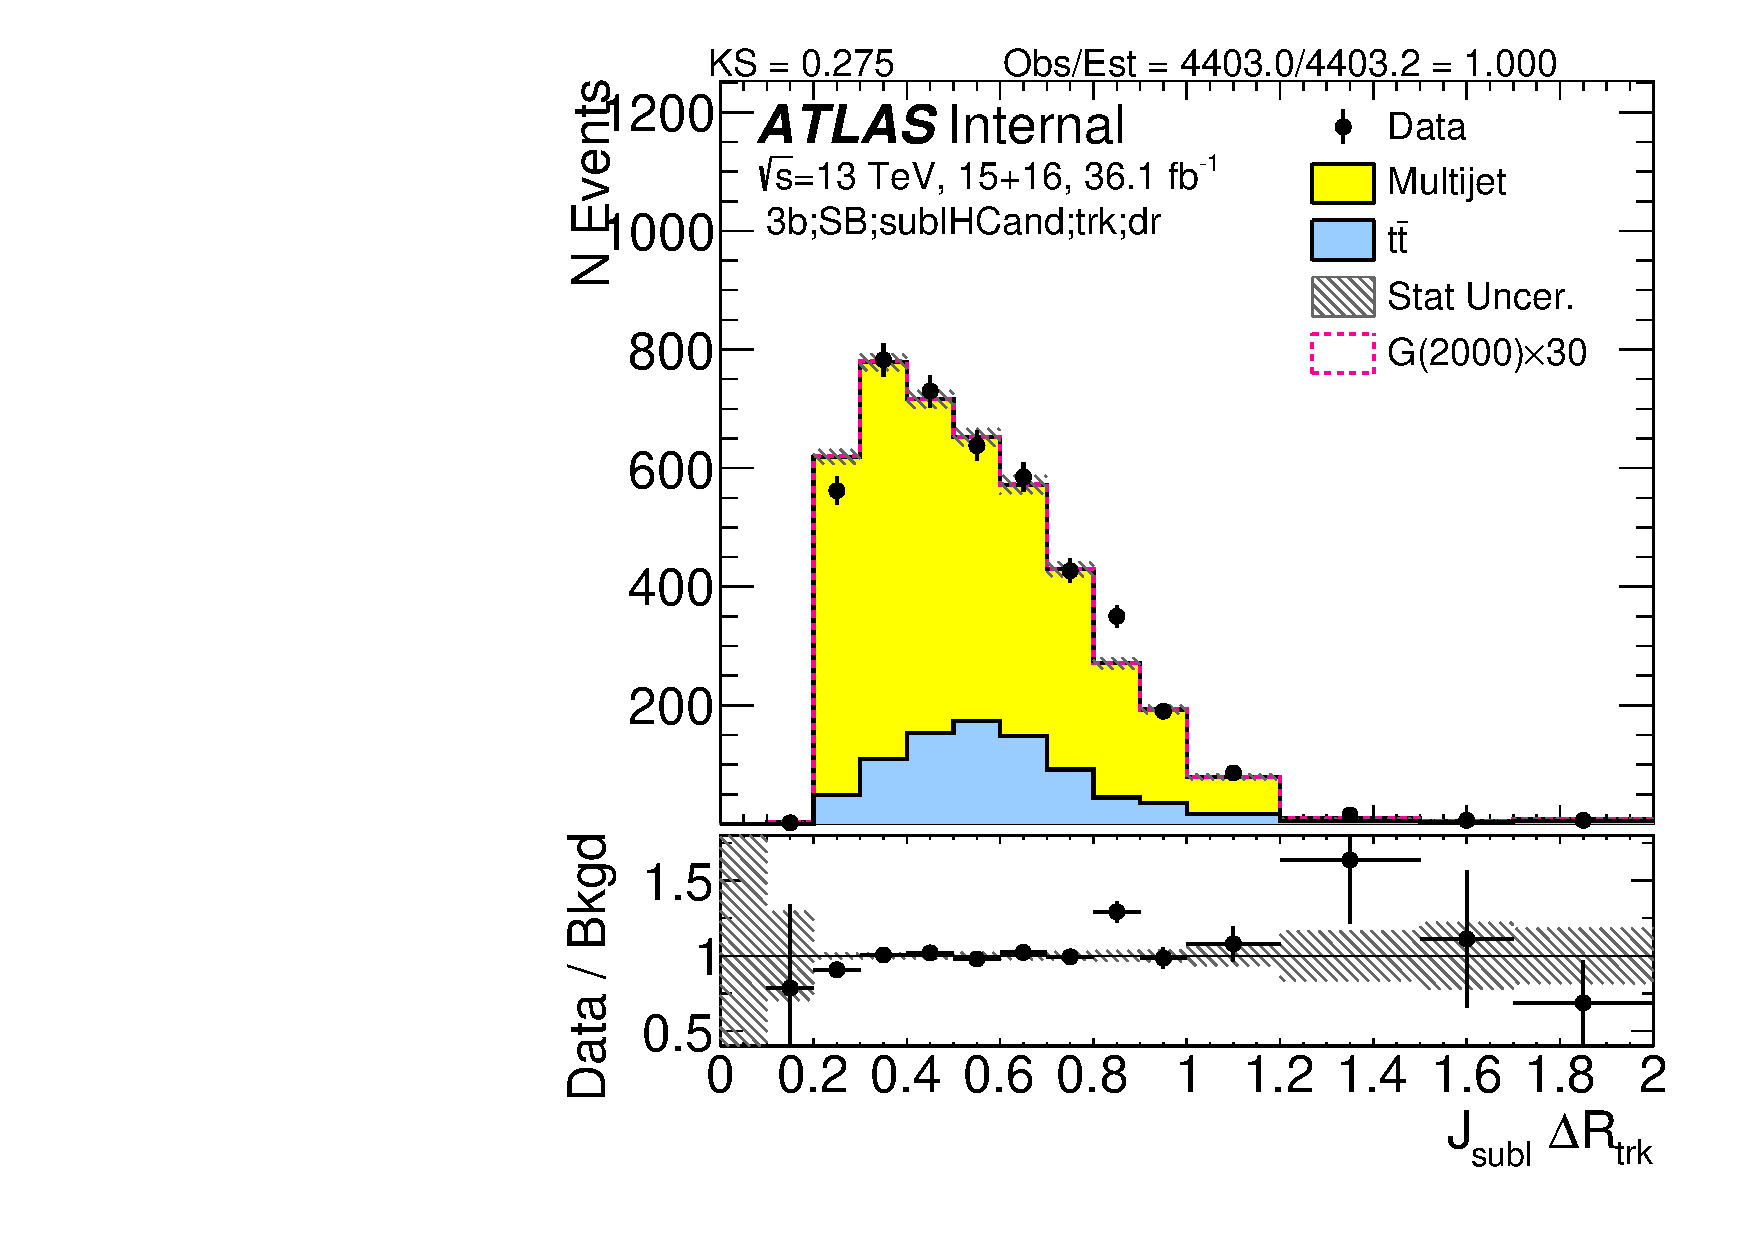
\includegraphics[width=0.32\textwidth,angle=-90]{figures/boosted/Sideband/b77_ThreeTag_Sideband_sublHCand_trk_dr.pdf}
  \caption{First two rows show the \pt~ of the lead (left) and sub-lead (right) small-$R$ track jets associated to the lead (first-row) and sub-lead (second-row) large-\R jet in data and prediction in the sideband region after requiring 3 $b$-tags. Third row shows the $\Delta R$ between two leading small-$R$ track-jets associated to the leading (left) and sub-leading (right) large-\R jet. }
  \label{fig:boosted-3b-sideband-ak2}
\end{center}
\end{figure*}


\begin{figure*}[htbp!]
\begin{center}
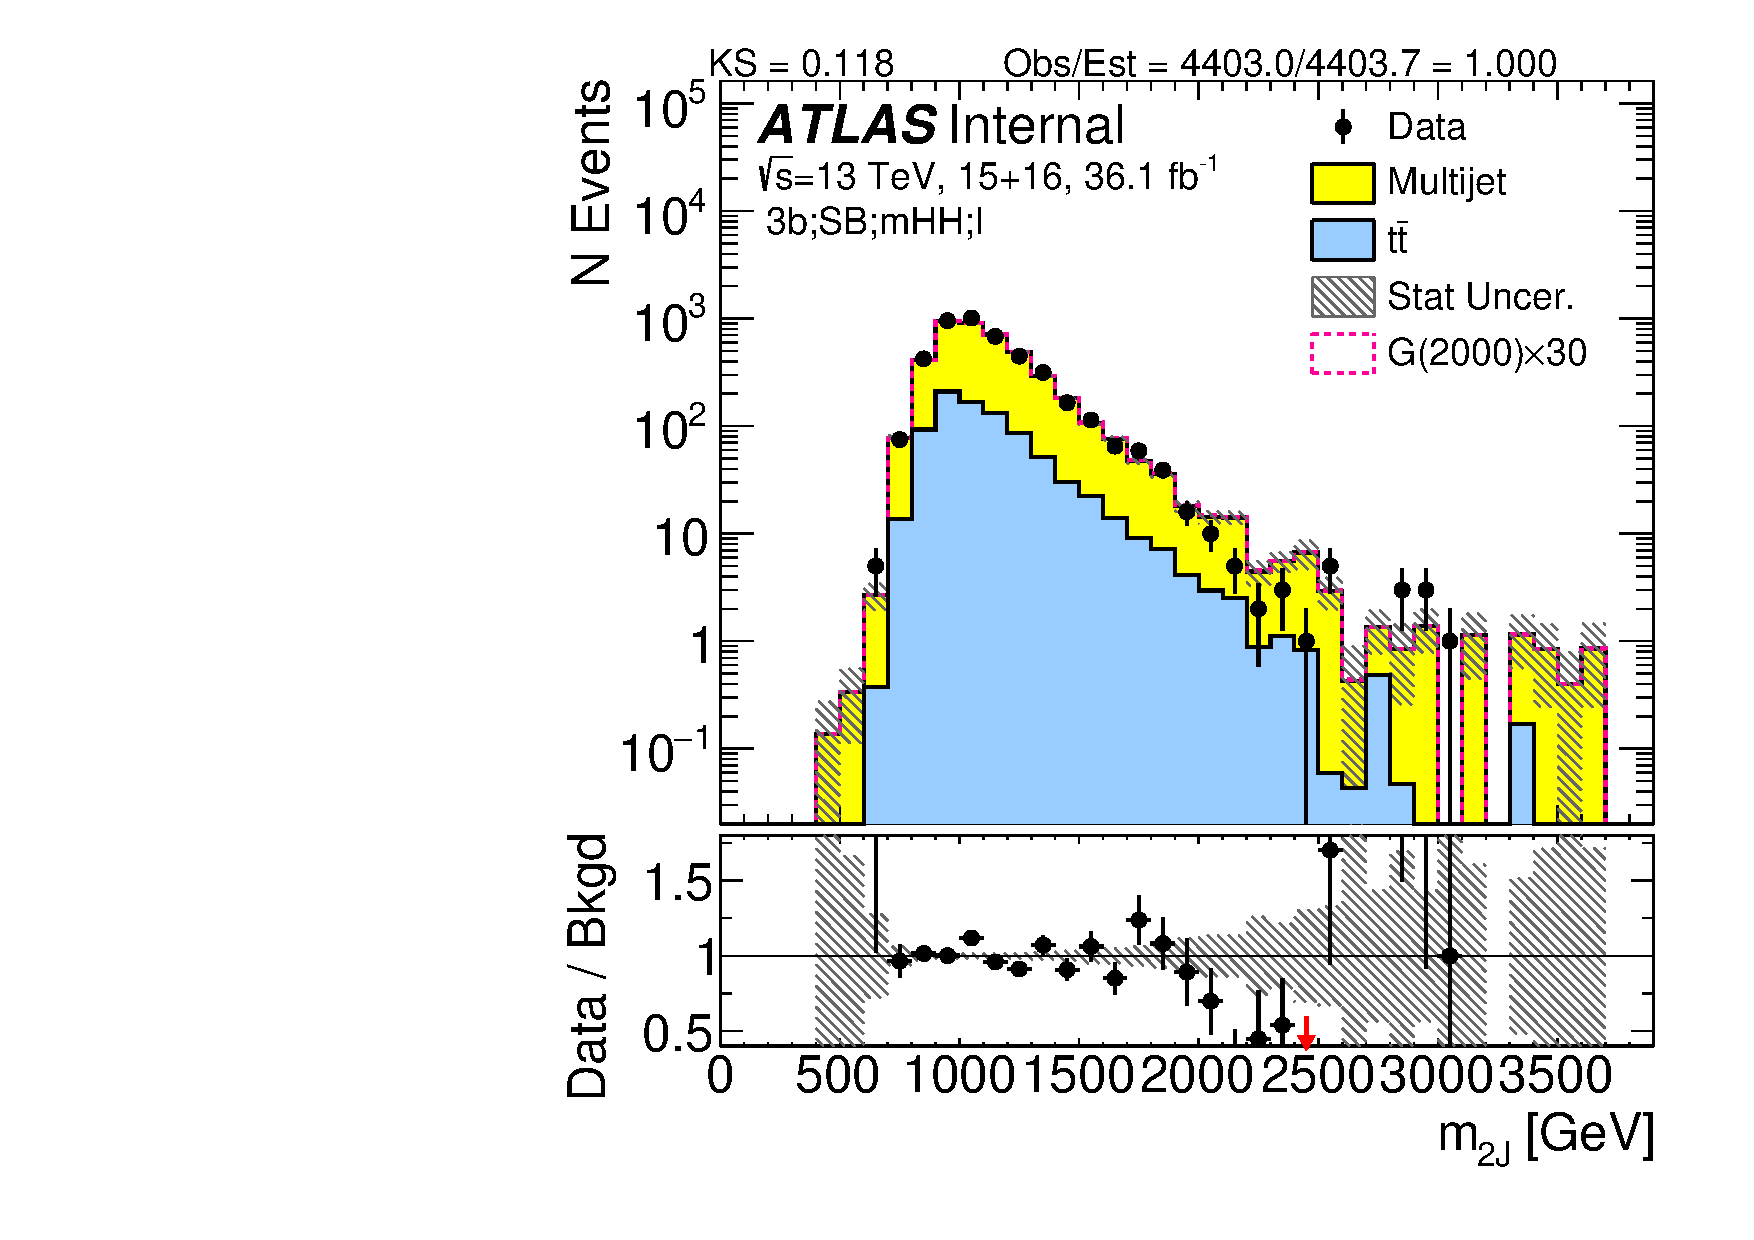
\includegraphics[width=0.32\textwidth,angle=-90]{figures/boosted/Sideband/b77_ThreeTag_Sideband_mHH_l_1.pdf}
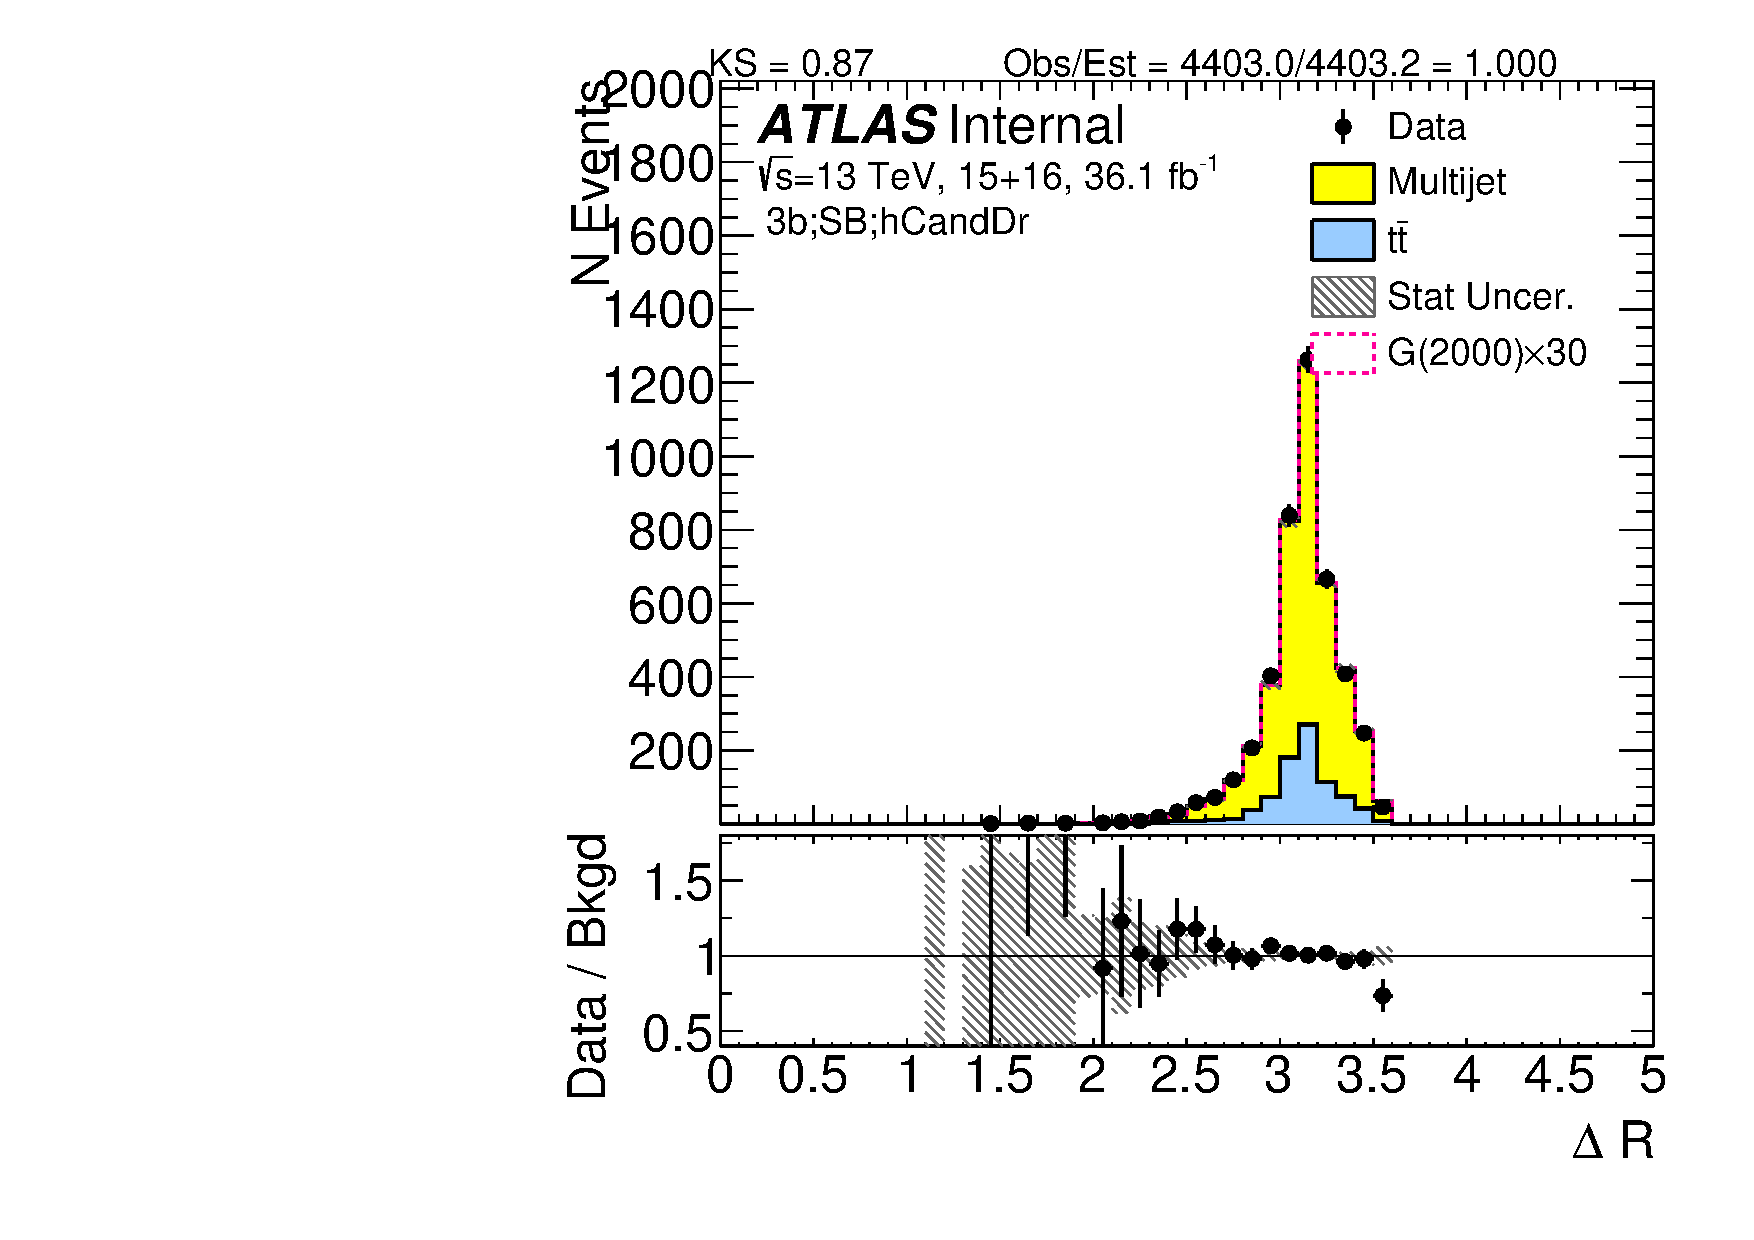
\includegraphics[width=0.32\textwidth,angle=-90]{figures/boosted/Sideband/b77_ThreeTag_Sideband_hCandDr.pdf}\\
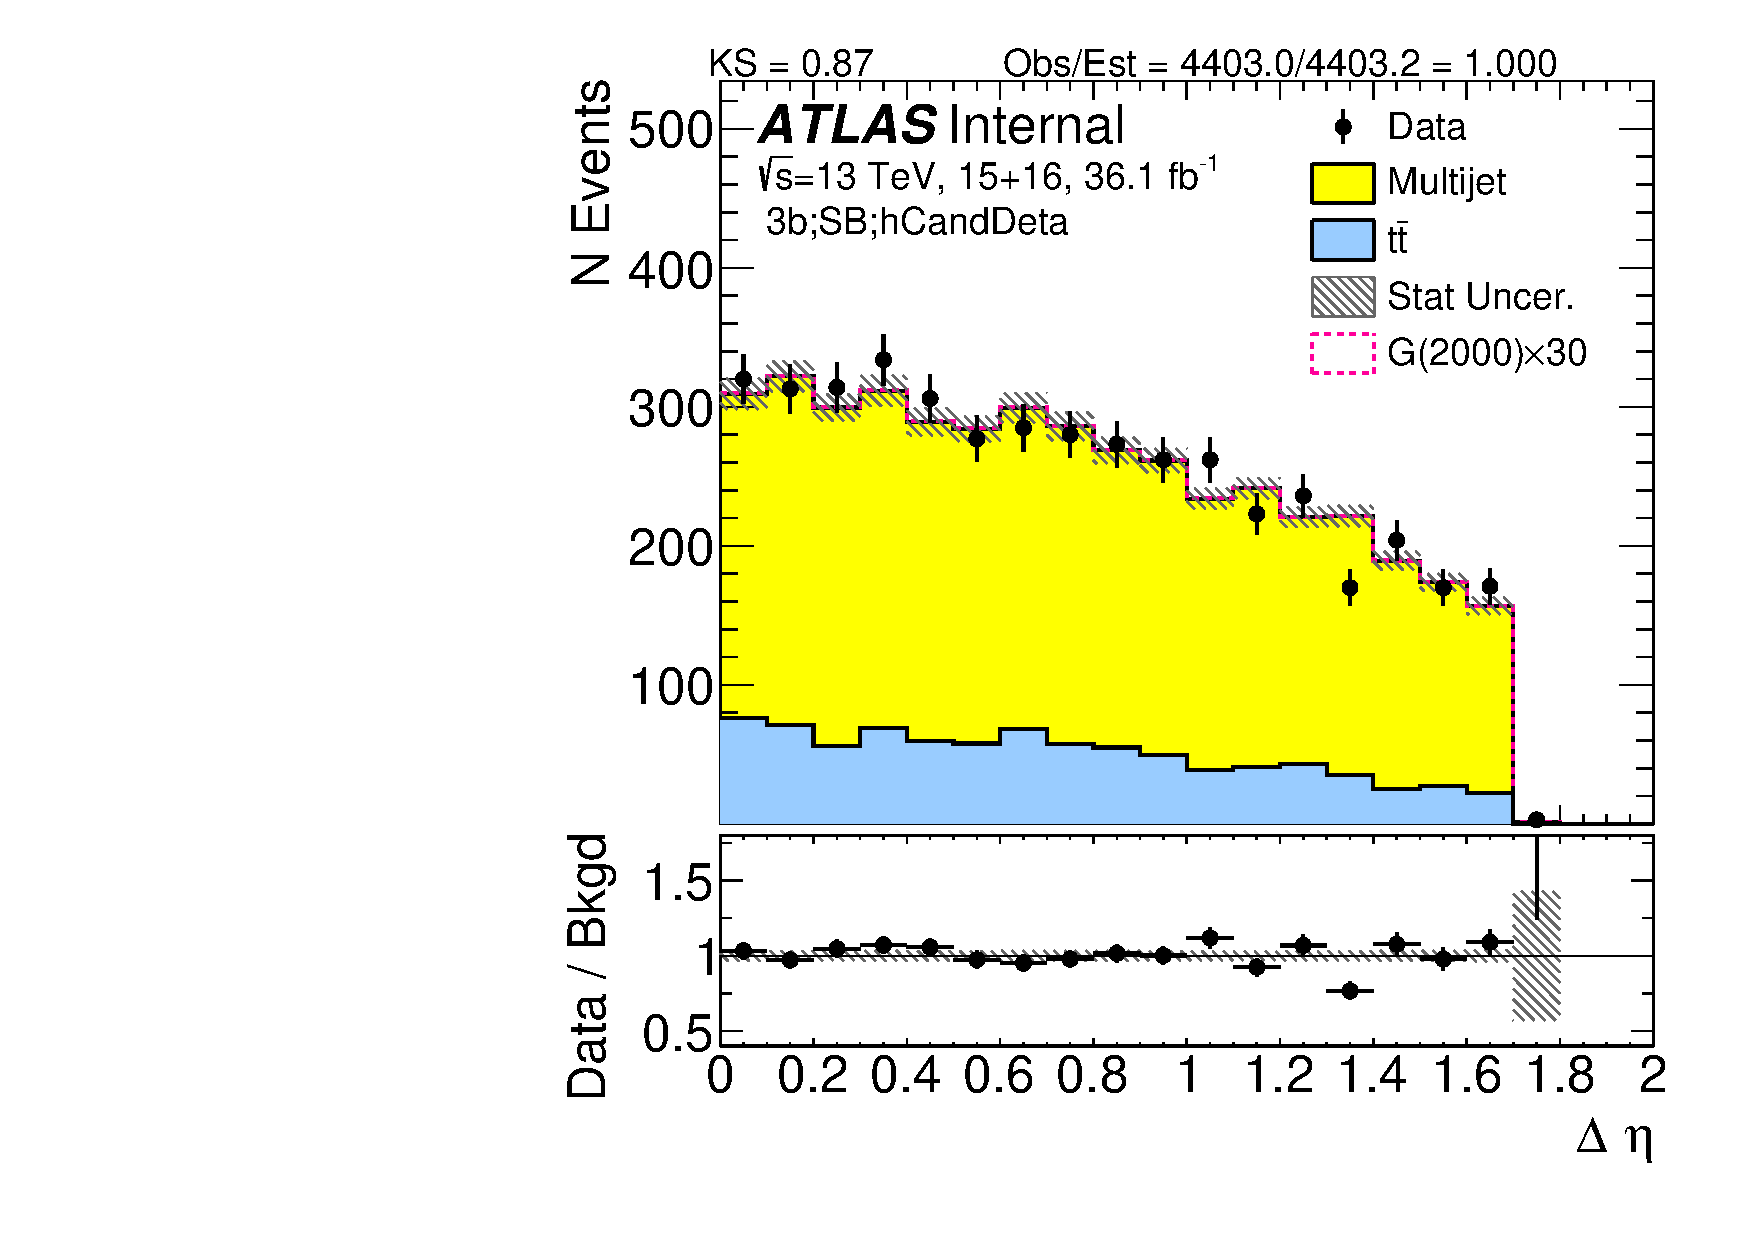
\includegraphics[width=0.32\textwidth,angle=-90]{figures/boosted/Sideband/b77_ThreeTag_Sideband_hCandDeta.pdf}
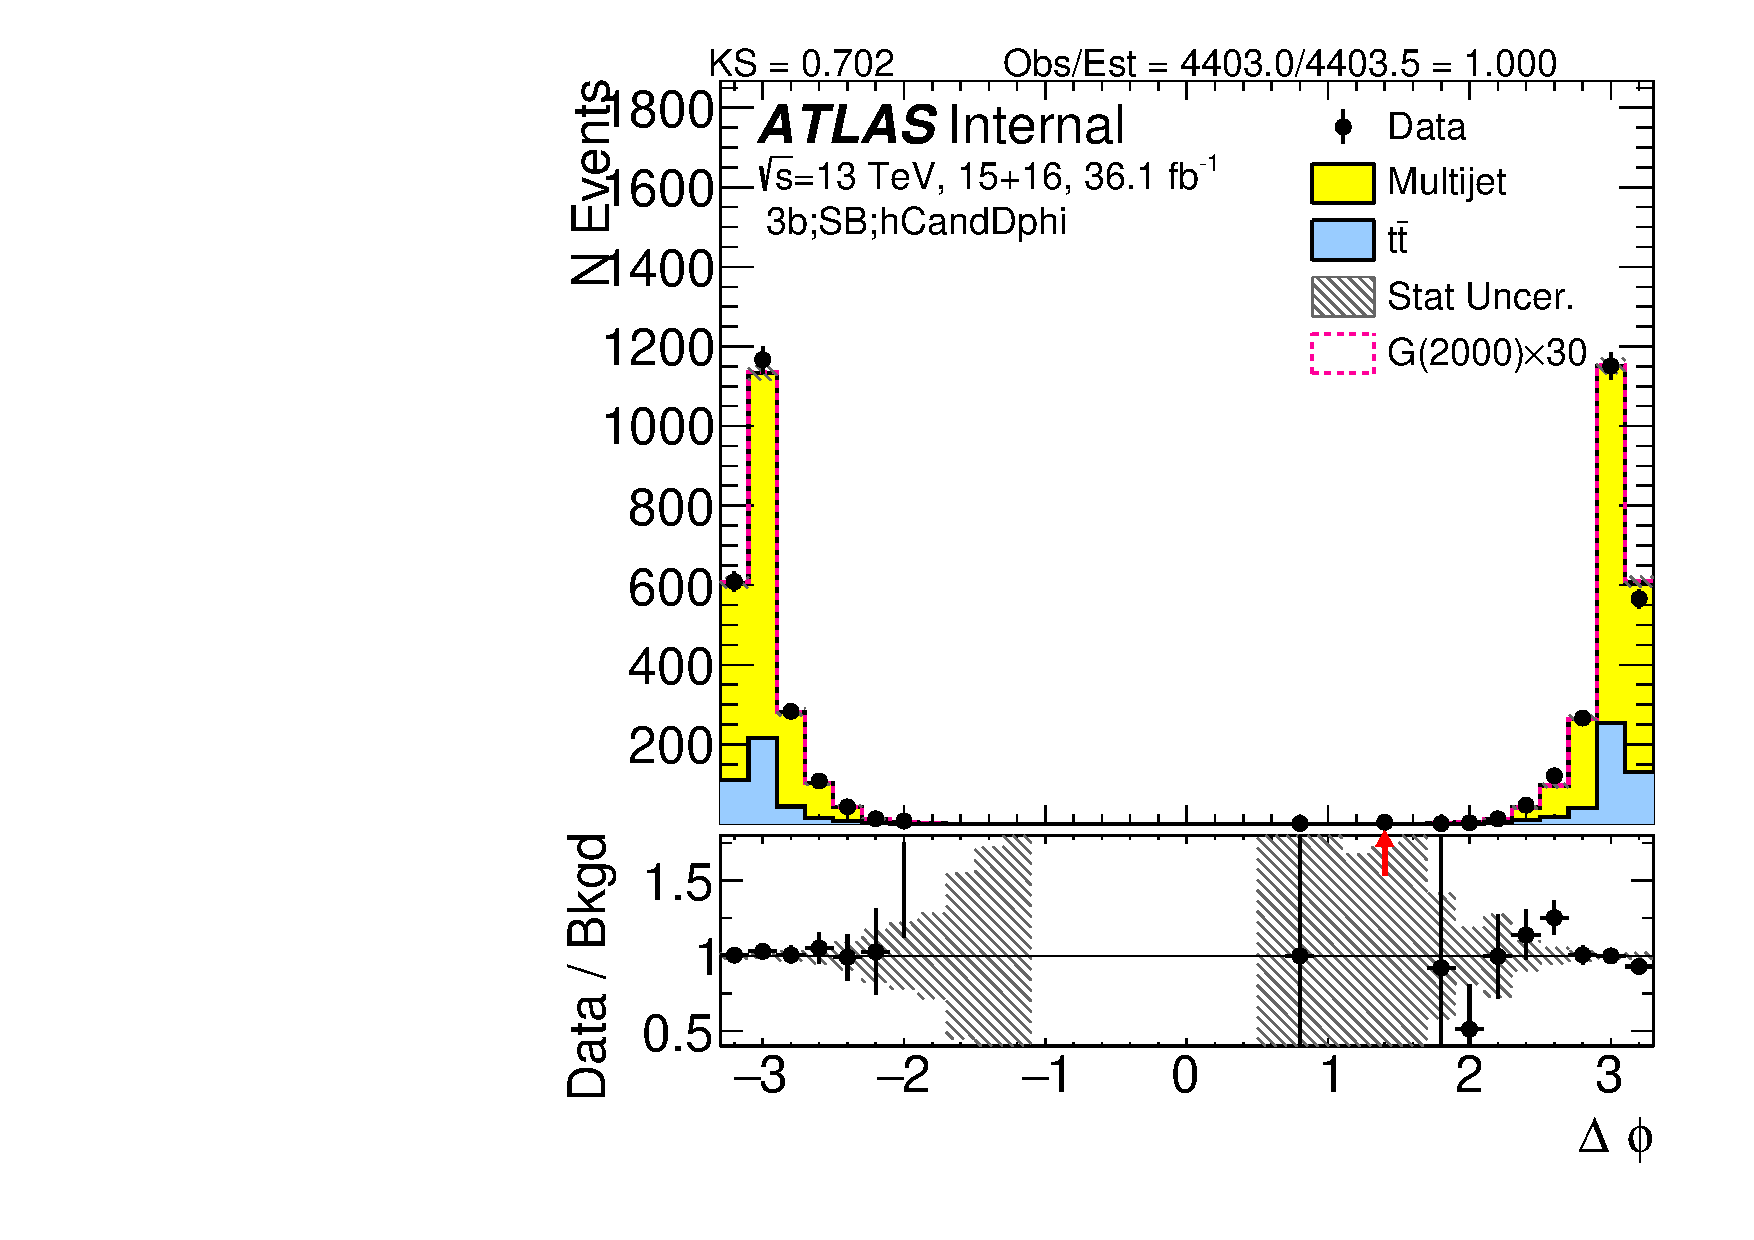
\includegraphics[width=0.32\textwidth,angle=-90]{figures/boosted/Sideband/b77_ThreeTag_Sideband_hCandDphi.pdf}
  \caption{Kinematics (invariant mass, $\Delta R$, $\Delta \eta$ and $\Delta \phi$) of two large-\R jets in data and prediction in the sideband region after requiring 3 $b$-tags. }
  \label{fig:boosted-3b-sideband-ak10-system}
\end{center}
\end{figure*}

\clearpage

\begin{figure*}[htbp!]
\begin{center}
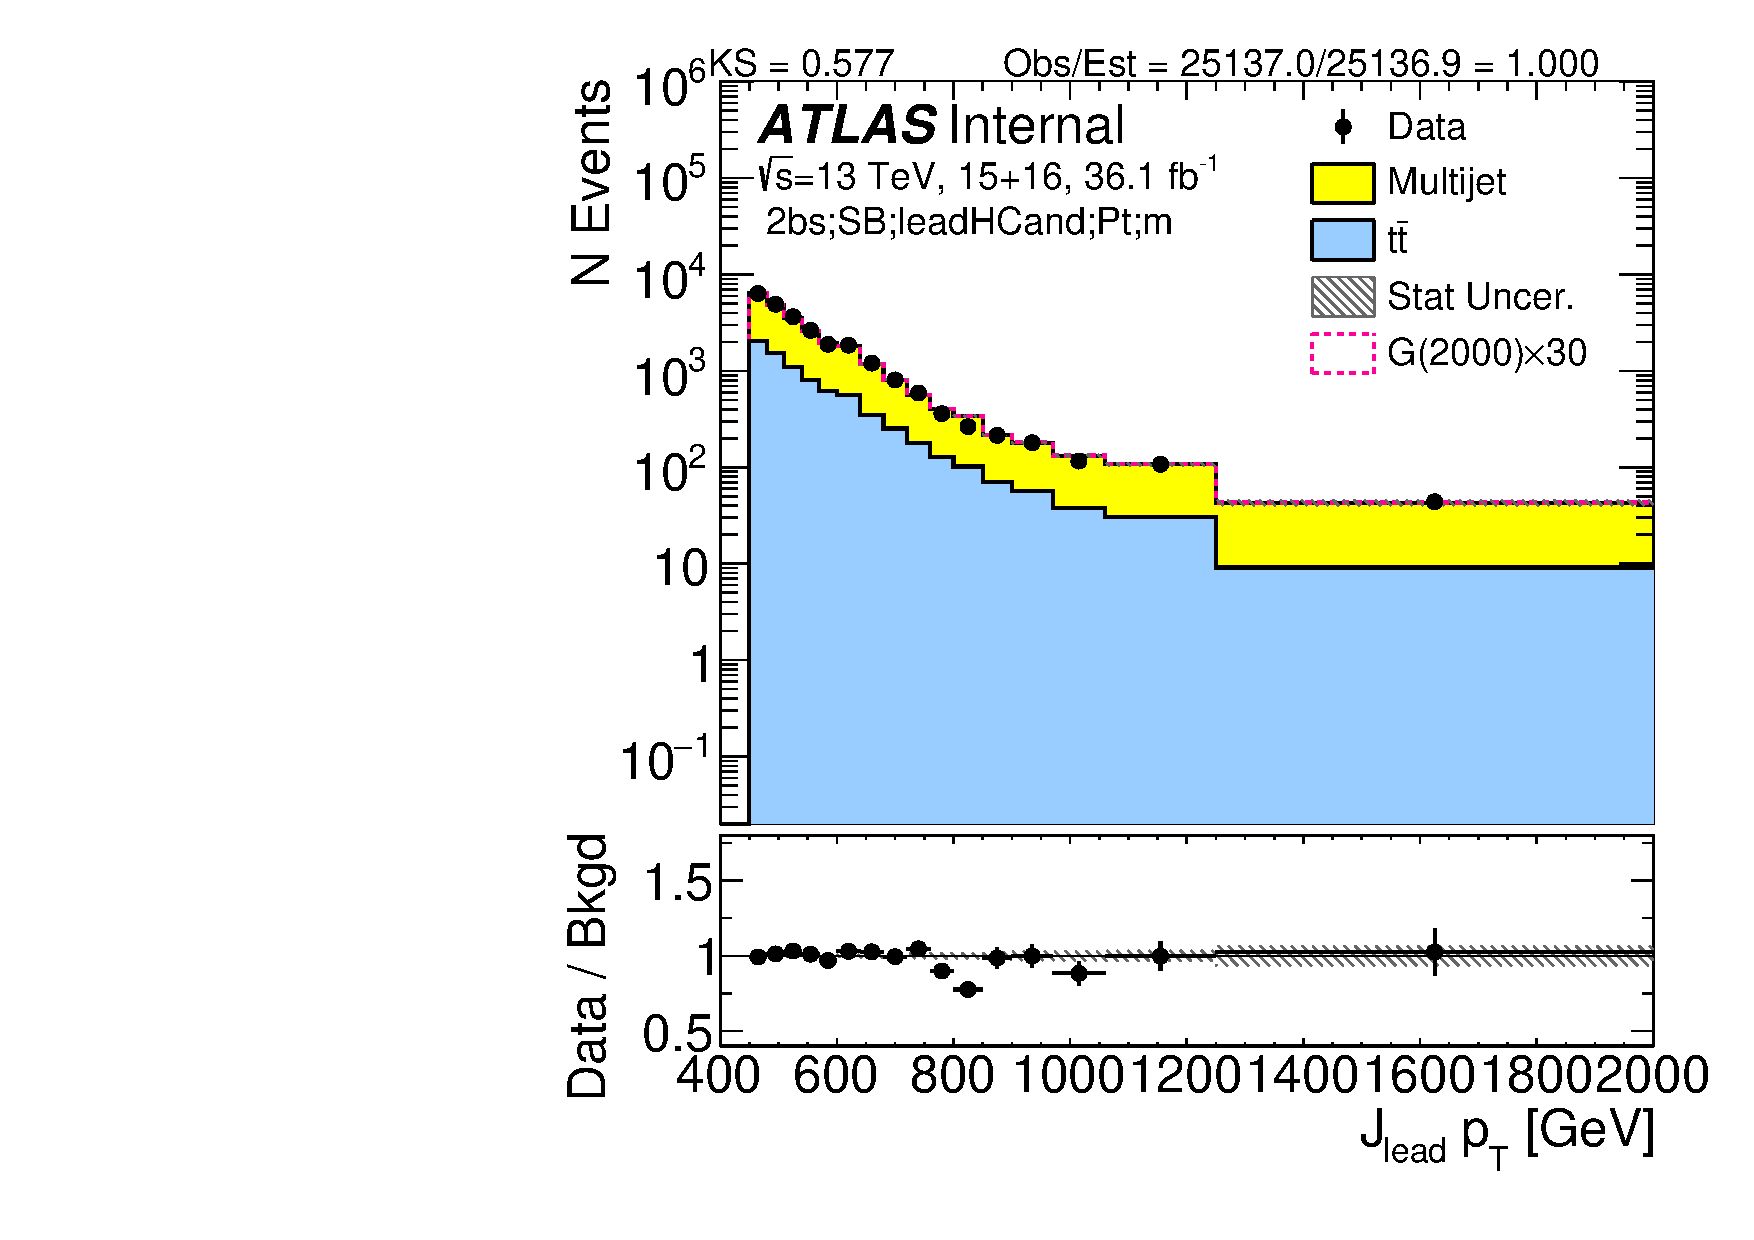
\includegraphics[width=0.32\textwidth,angle=-90]{figures/boosted/Sideband/b77_TwoTag_split_Sideband_leadHCand_Pt_m_1.pdf}
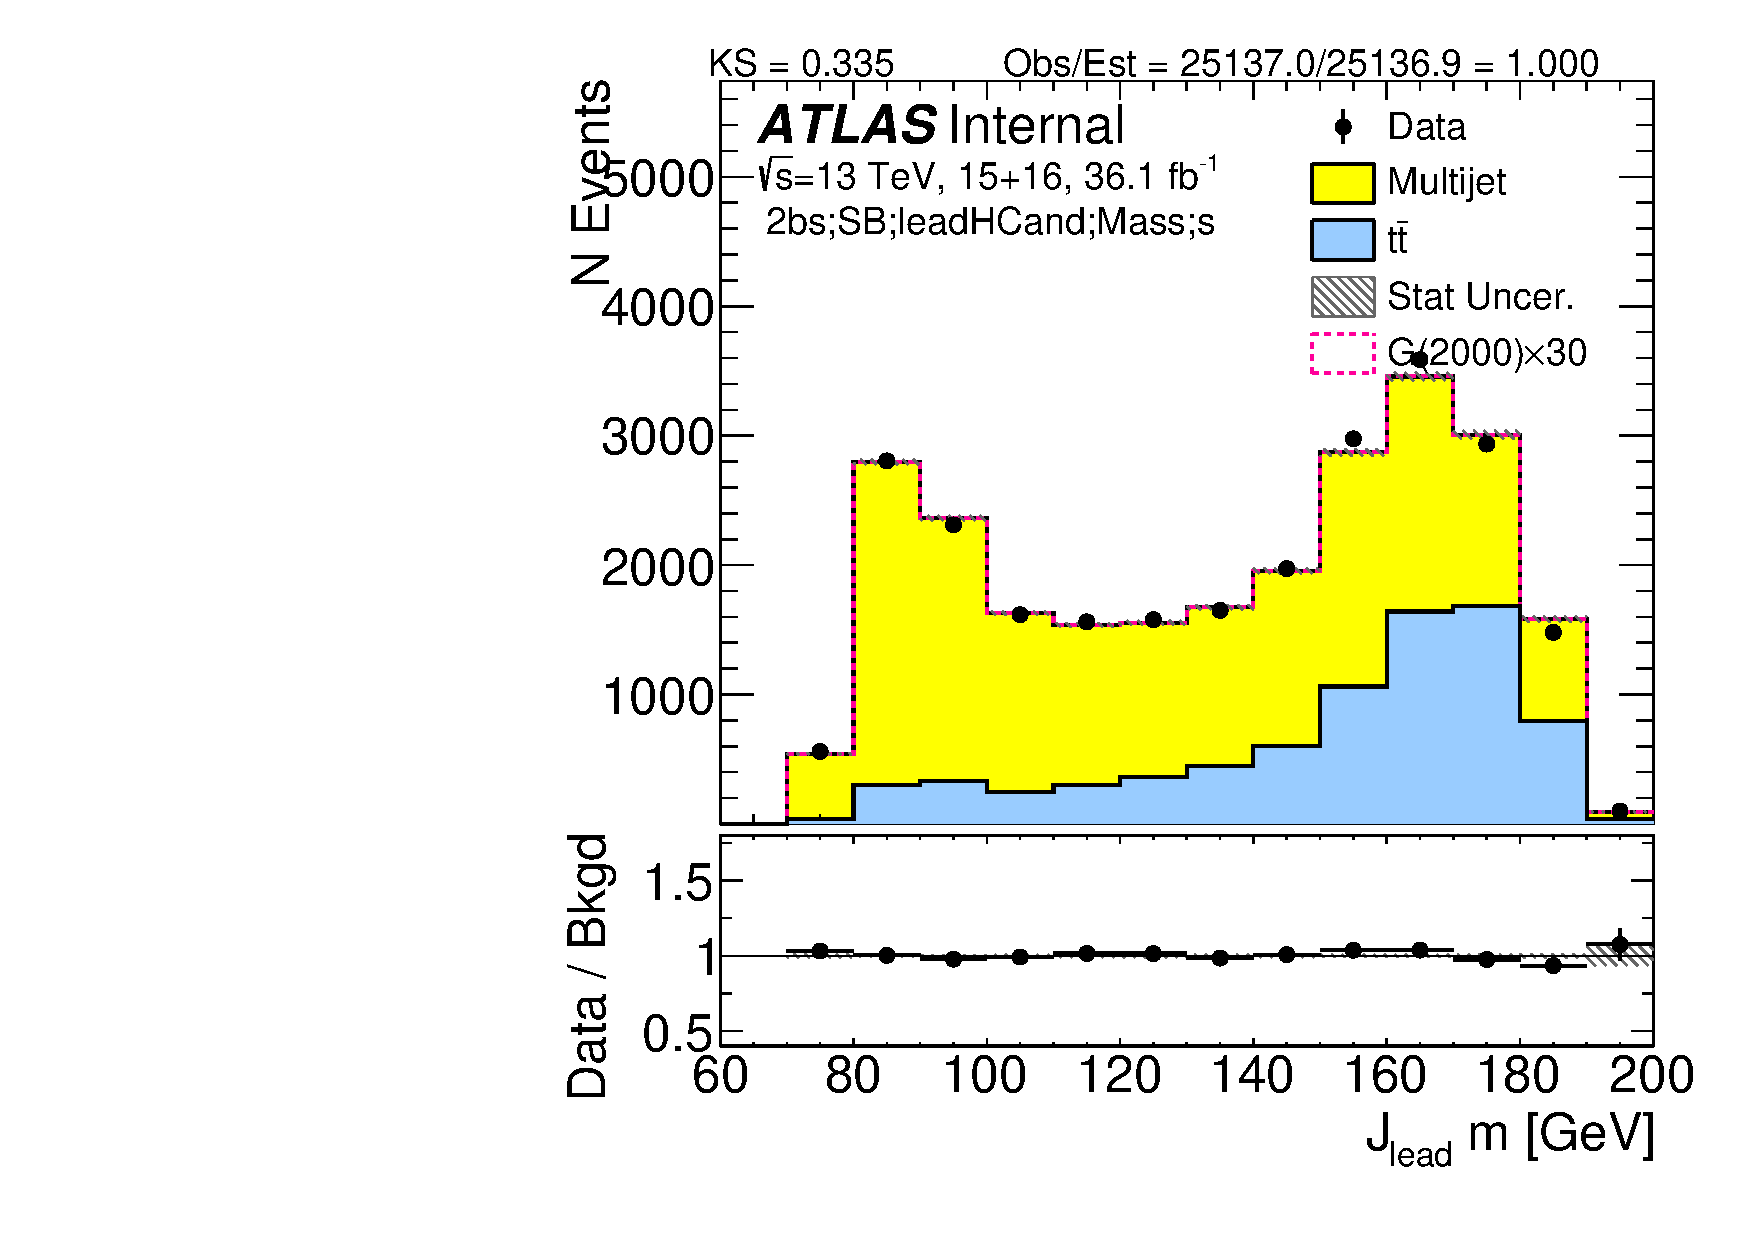
\includegraphics[width=0.32\textwidth,angle=-90]{figures/boosted/Sideband/b77_TwoTag_split_Sideband_leadHCand_Mass_s.pdf}\\
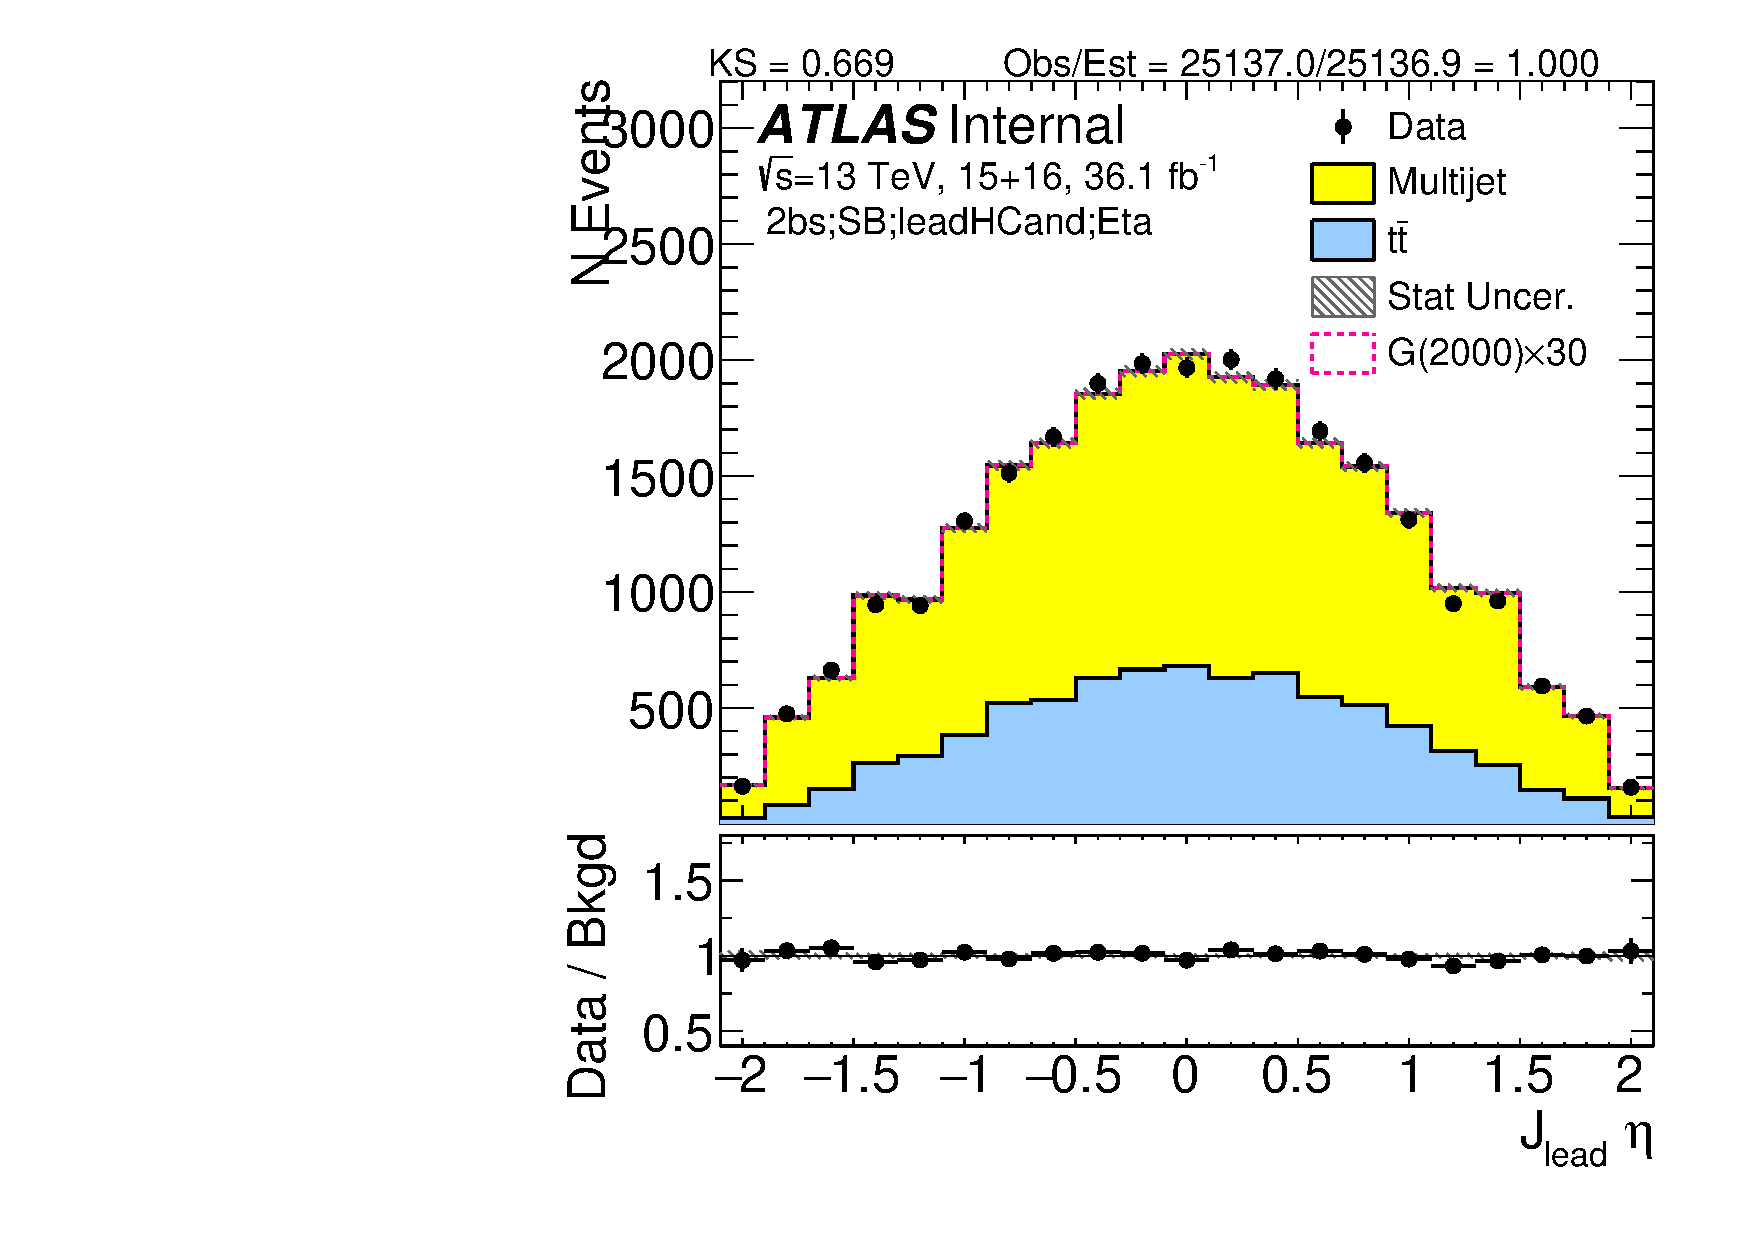
\includegraphics[width=0.32\textwidth,angle=-90]{figures/boosted/Sideband/b77_TwoTag_split_Sideband_leadHCand_Eta.pdf}
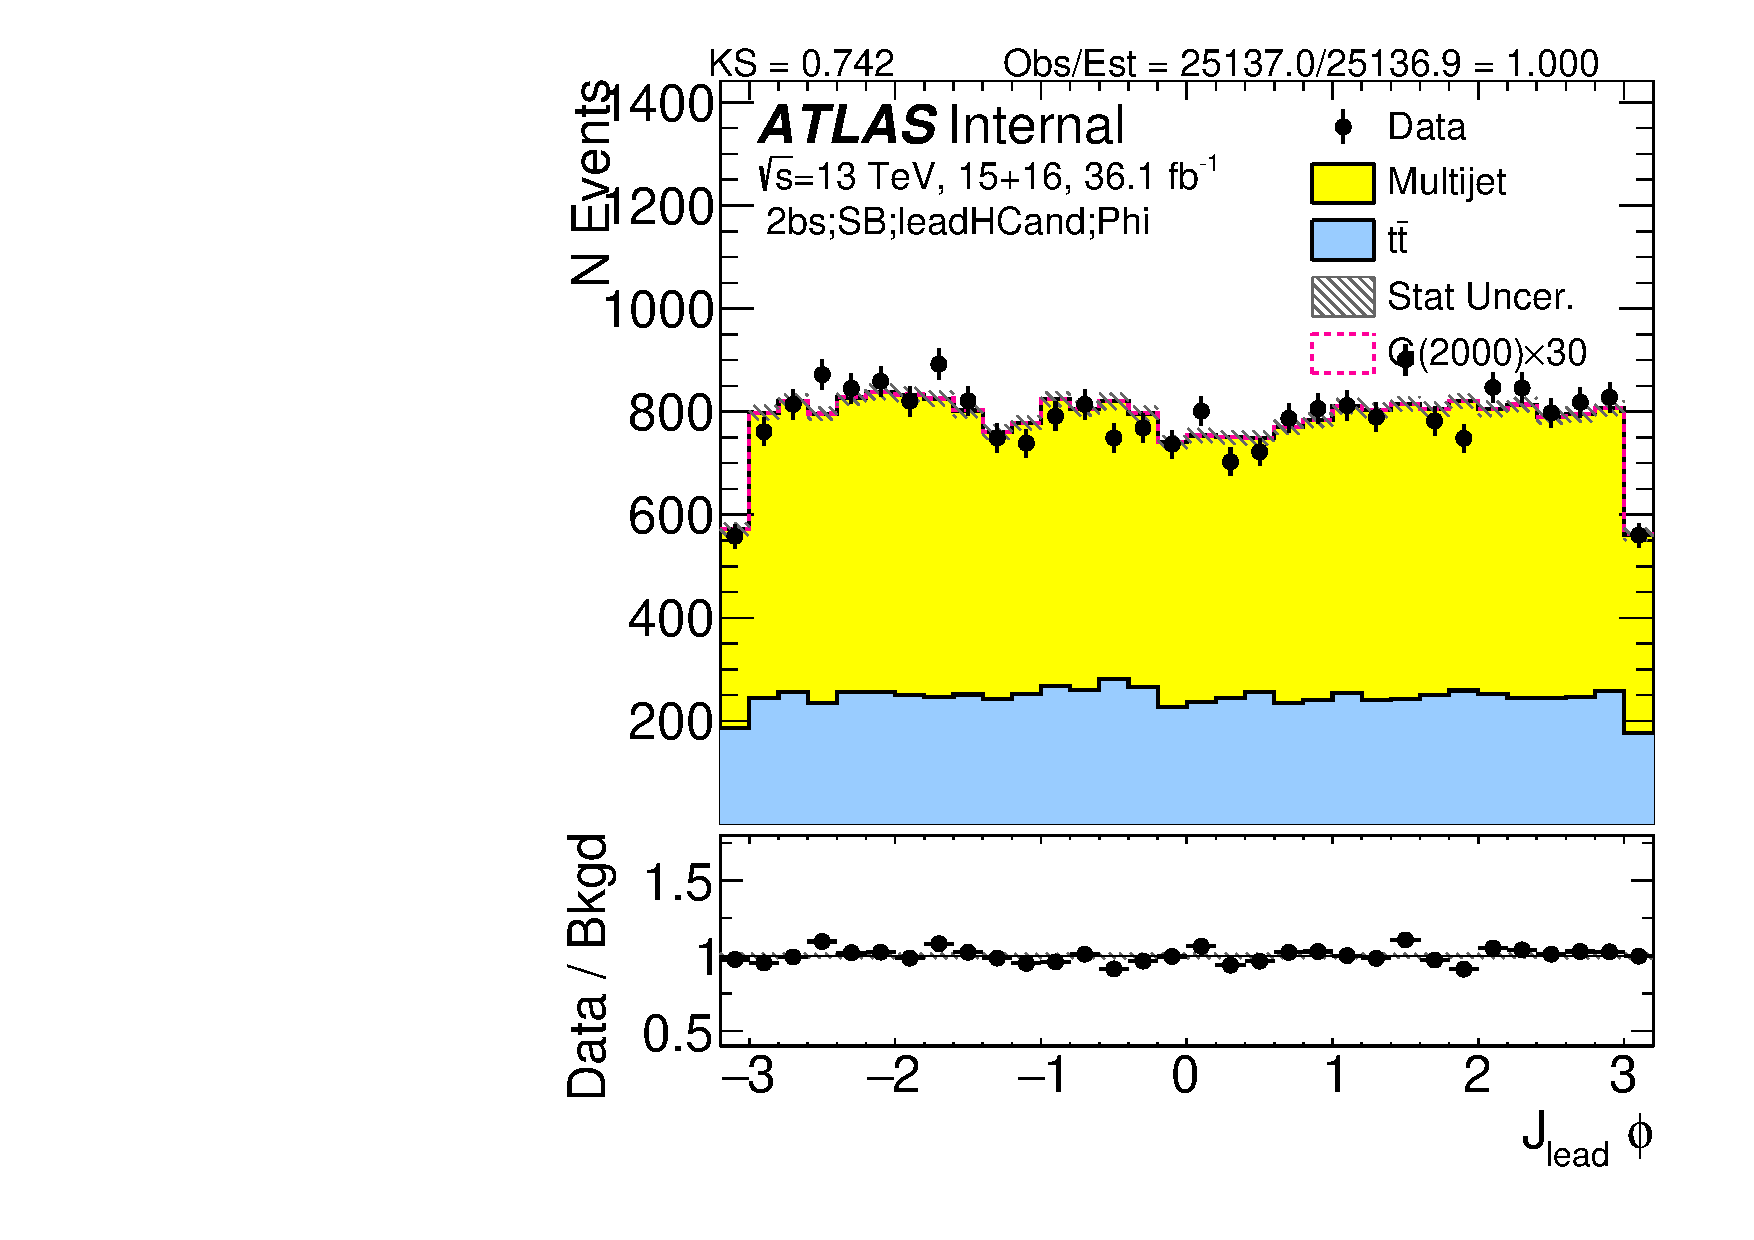
\includegraphics[width=0.32\textwidth,angle=-90]{figures/boosted/Sideband/b77_TwoTag_split_Sideband_leadHCand_Phi.pdf}
  \caption{Kinematics (\pt~, mass, $\eta$, $\phi$) of the lead large-\R jet in data and prediction in the sideband region after requiring 2 $b$-tags split.}
  \label{fig:boosted-2bs-sideband-ak10-lead}
\end{center}
\end{figure*}

\begin{figure*}[htbp!]
\begin{center}
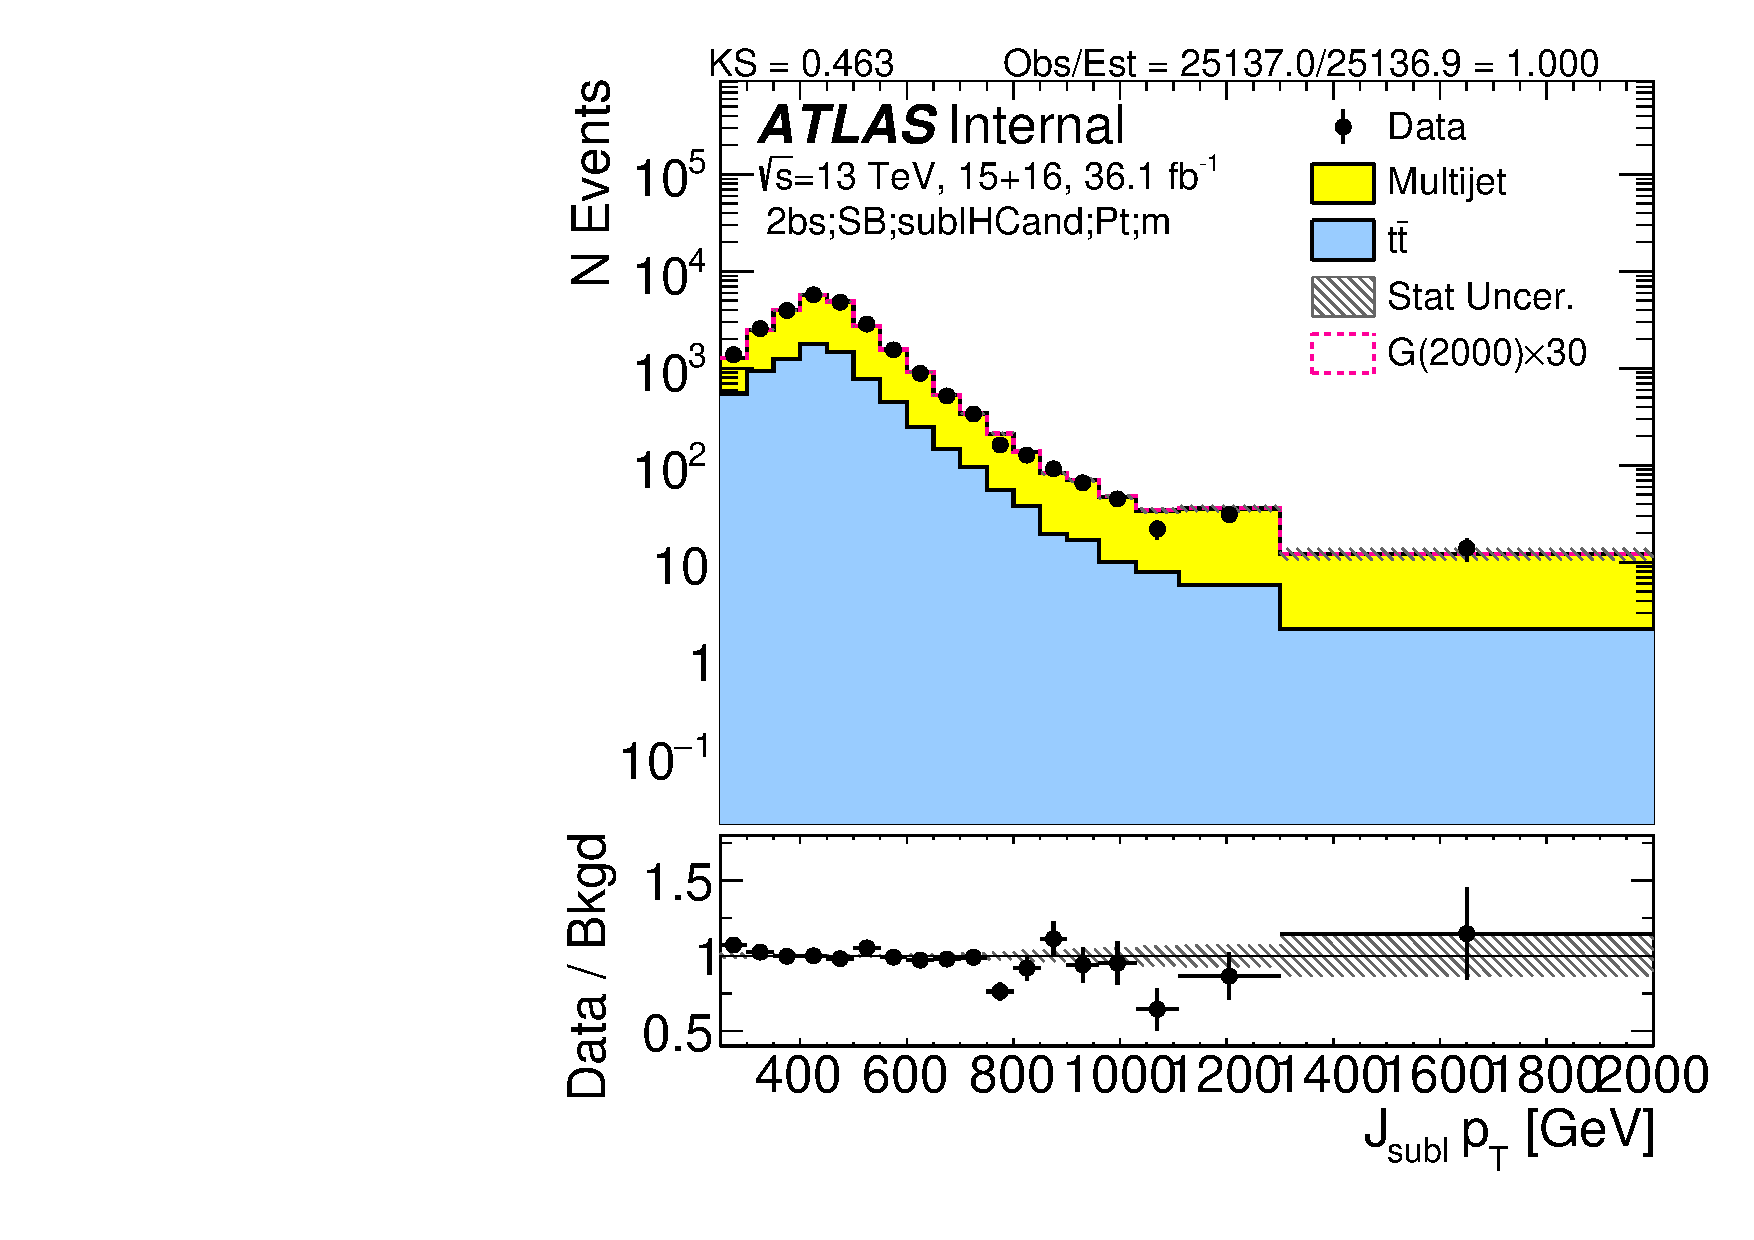
\includegraphics[width=0.32\textwidth,angle=-90]{figures/boosted/Sideband/b77_TwoTag_split_Sideband_sublHCand_Pt_m_1.pdf}
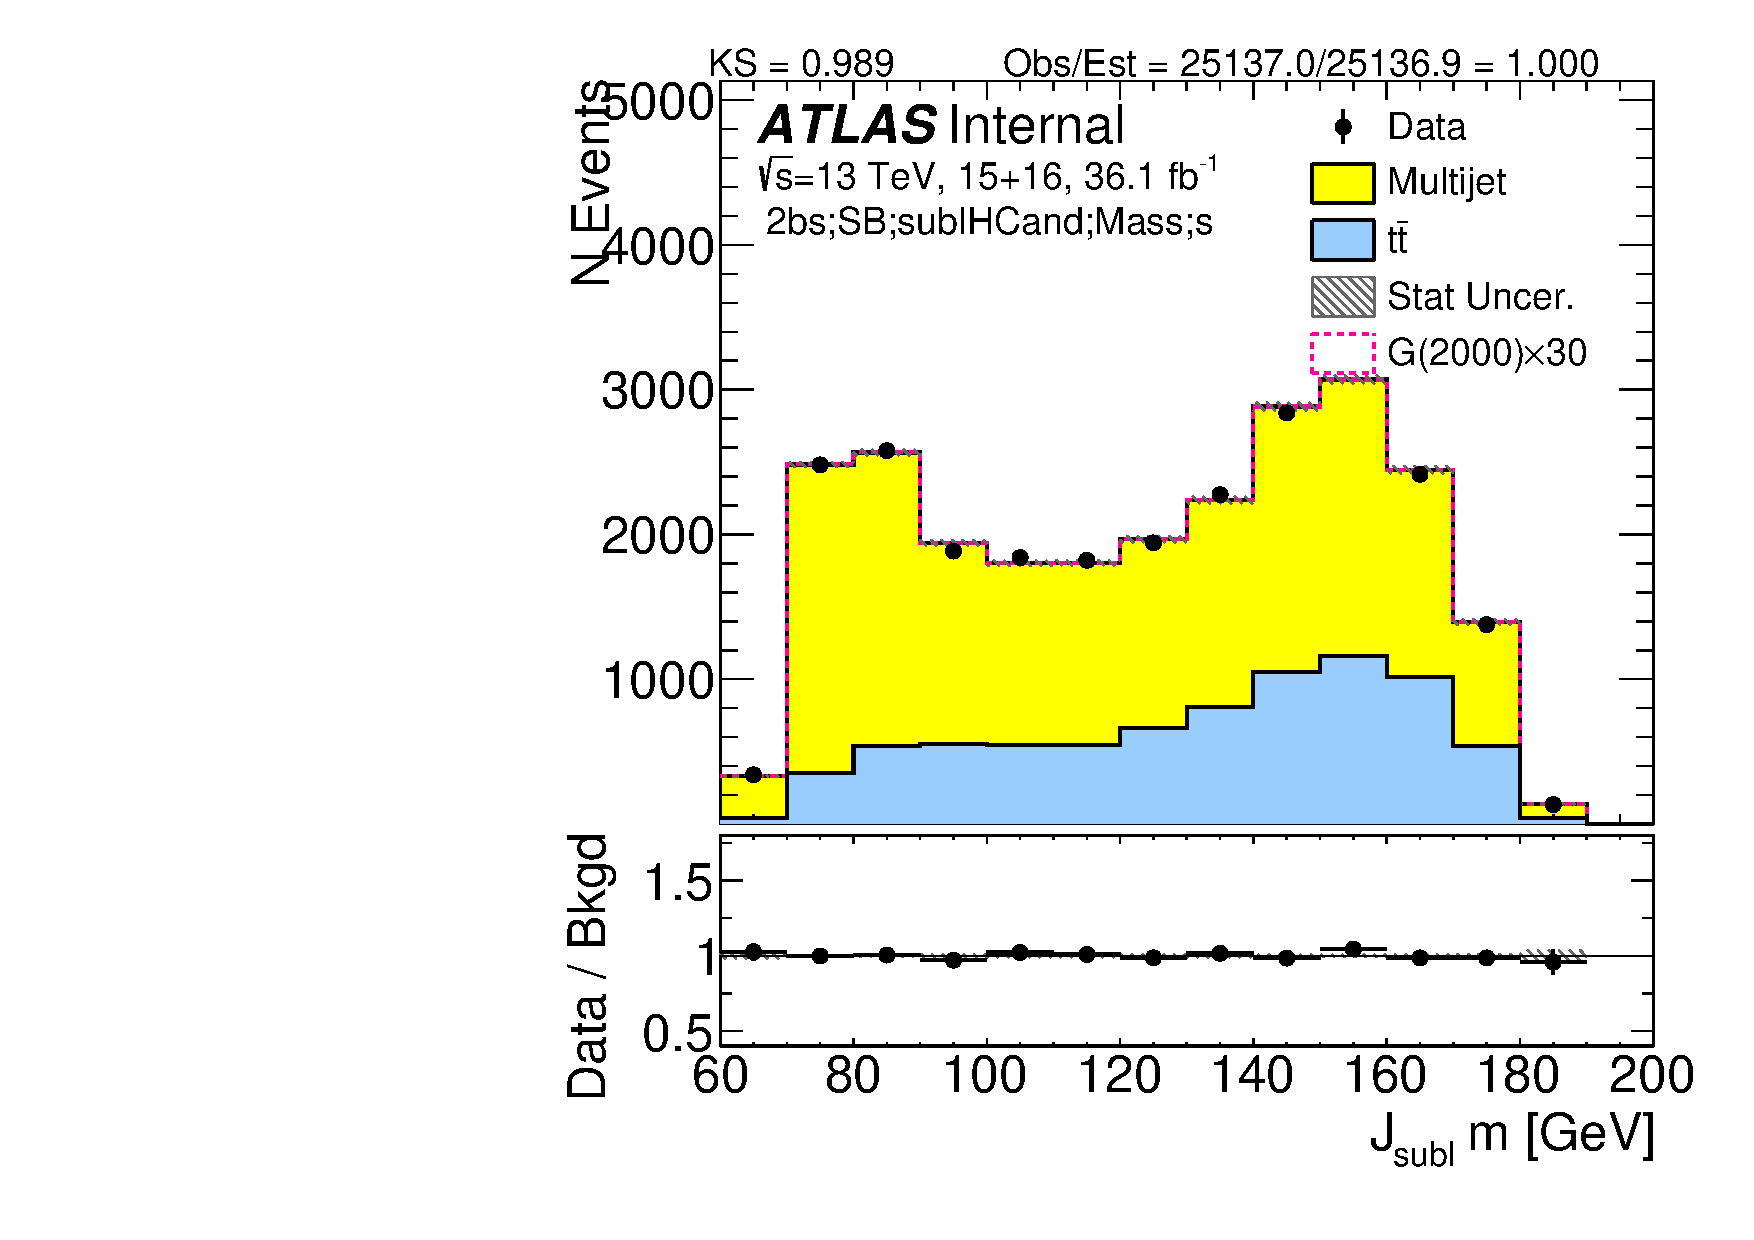
\includegraphics[width=0.32\textwidth,angle=-90]{figures/boosted/Sideband/b77_TwoTag_split_Sideband_sublHCand_Mass_s.pdf}\\
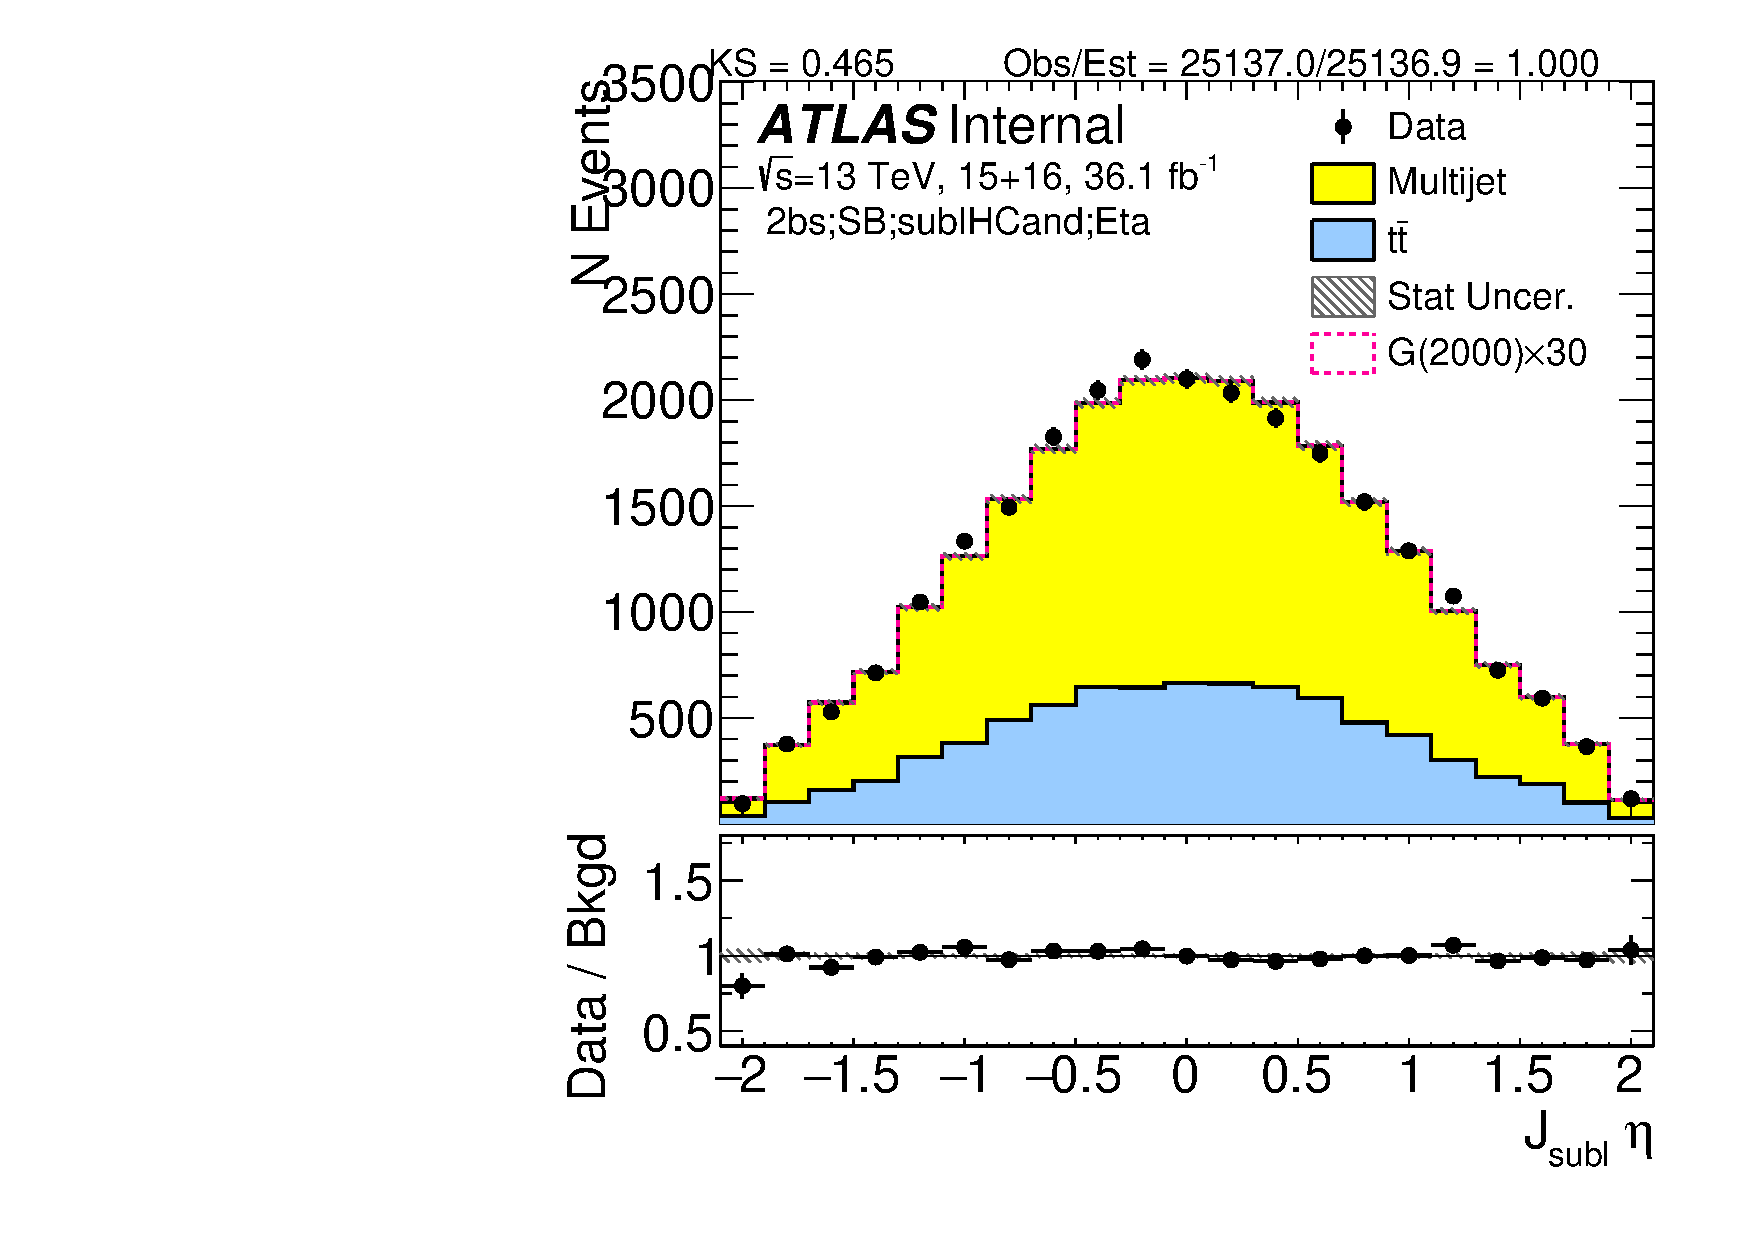
\includegraphics[width=0.32\textwidth,angle=-90]{figures/boosted/Sideband/b77_TwoTag_split_Sideband_sublHCand_Eta.pdf}
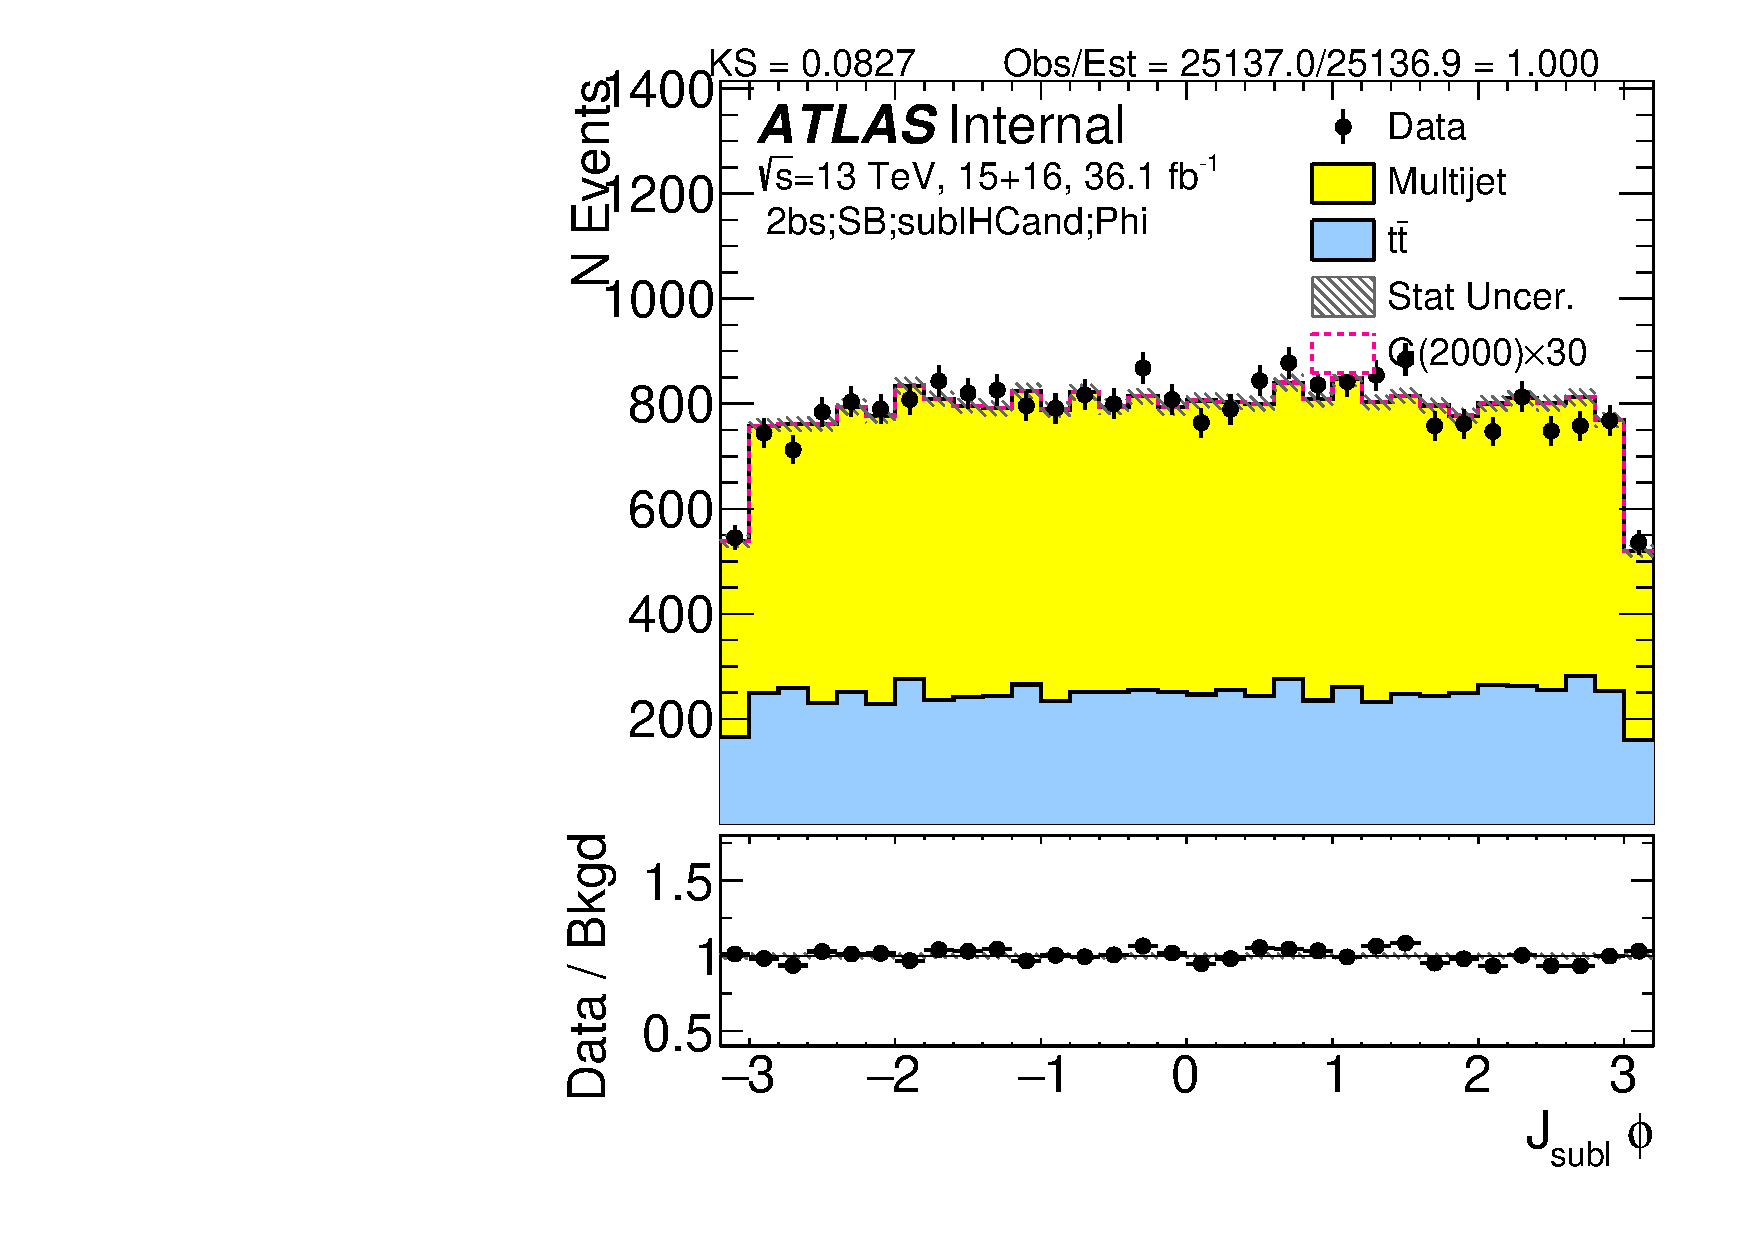
\includegraphics[width=0.32\textwidth,angle=-90]{figures/boosted/Sideband/b77_TwoTag_split_Sideband_sublHCand_Phi.pdf}
  \caption{Kinematics (\pt~, mass, $\eta$, $\phi$) of the subleading large-\R jet in data and prediction in the sideband region after requiring 2 $b$-tags split.}
  \label{fig:boosted-2bs-sideband-ak10-subl}
\end{center}
\end{figure*}

\begin{figure*}[htbp!]
\begin{center}
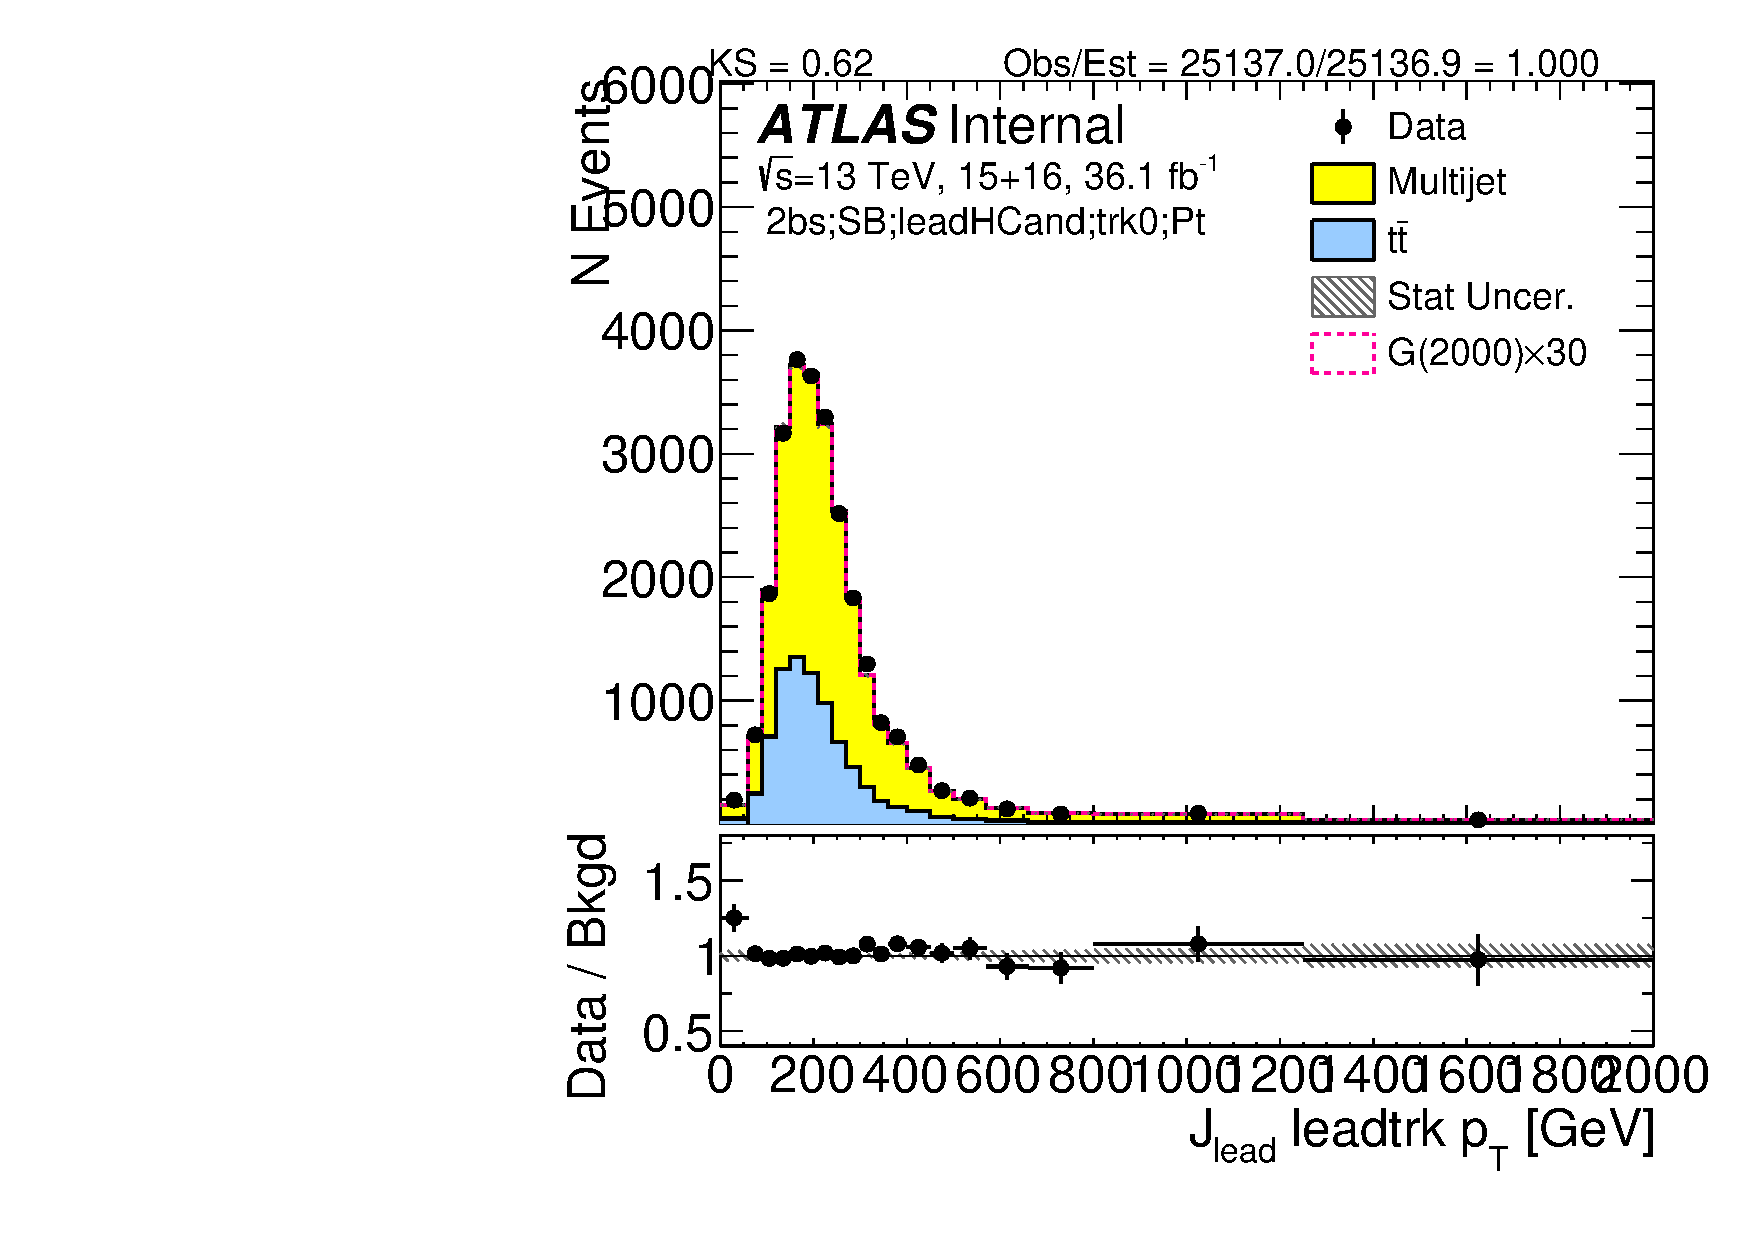
\includegraphics[width=0.32\textwidth,angle=-90]{figures/boosted/Sideband/b77_TwoTag_split_Sideband_leadHCand_trk0_Pt.pdf}
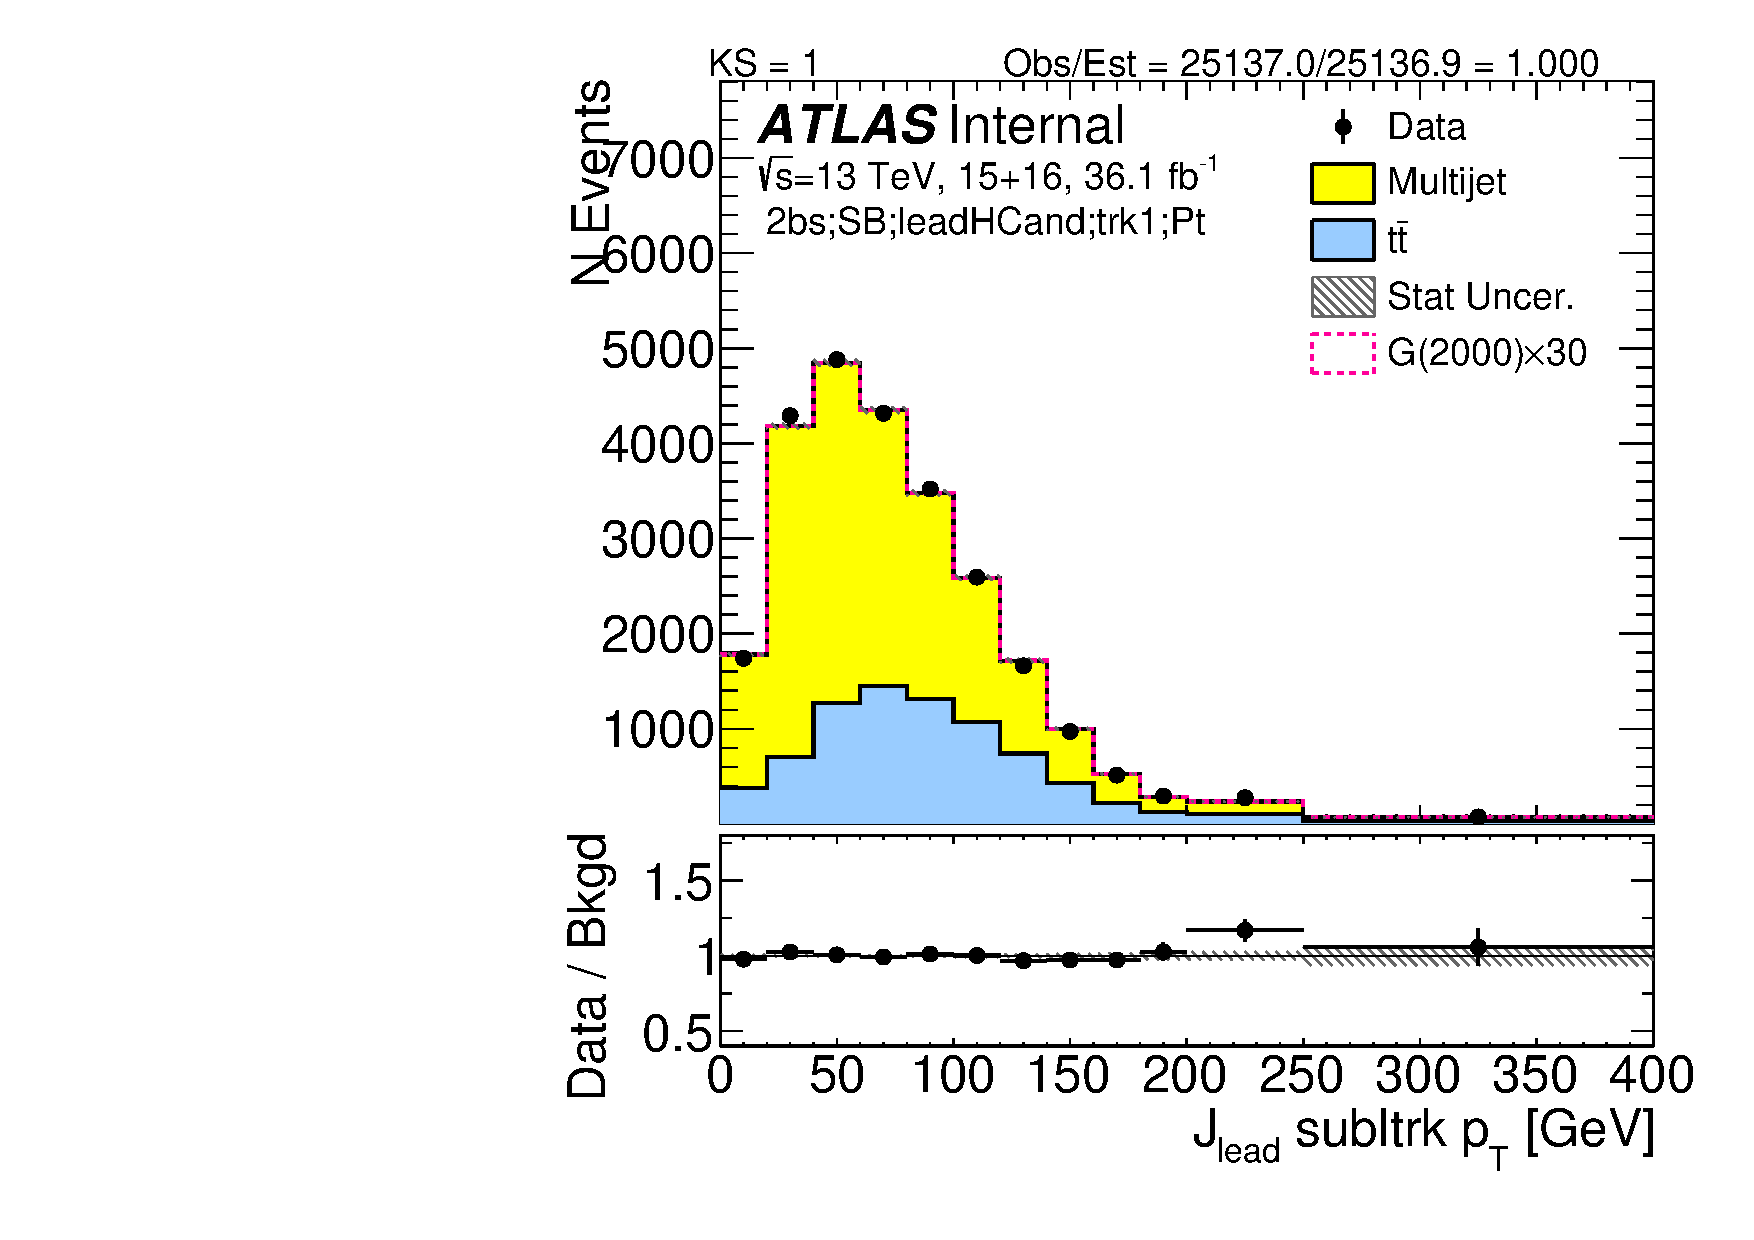
\includegraphics[width=0.32\textwidth,angle=-90]{figures/boosted/Sideband/b77_TwoTag_split_Sideband_leadHCand_trk1_Pt.pdf}\\
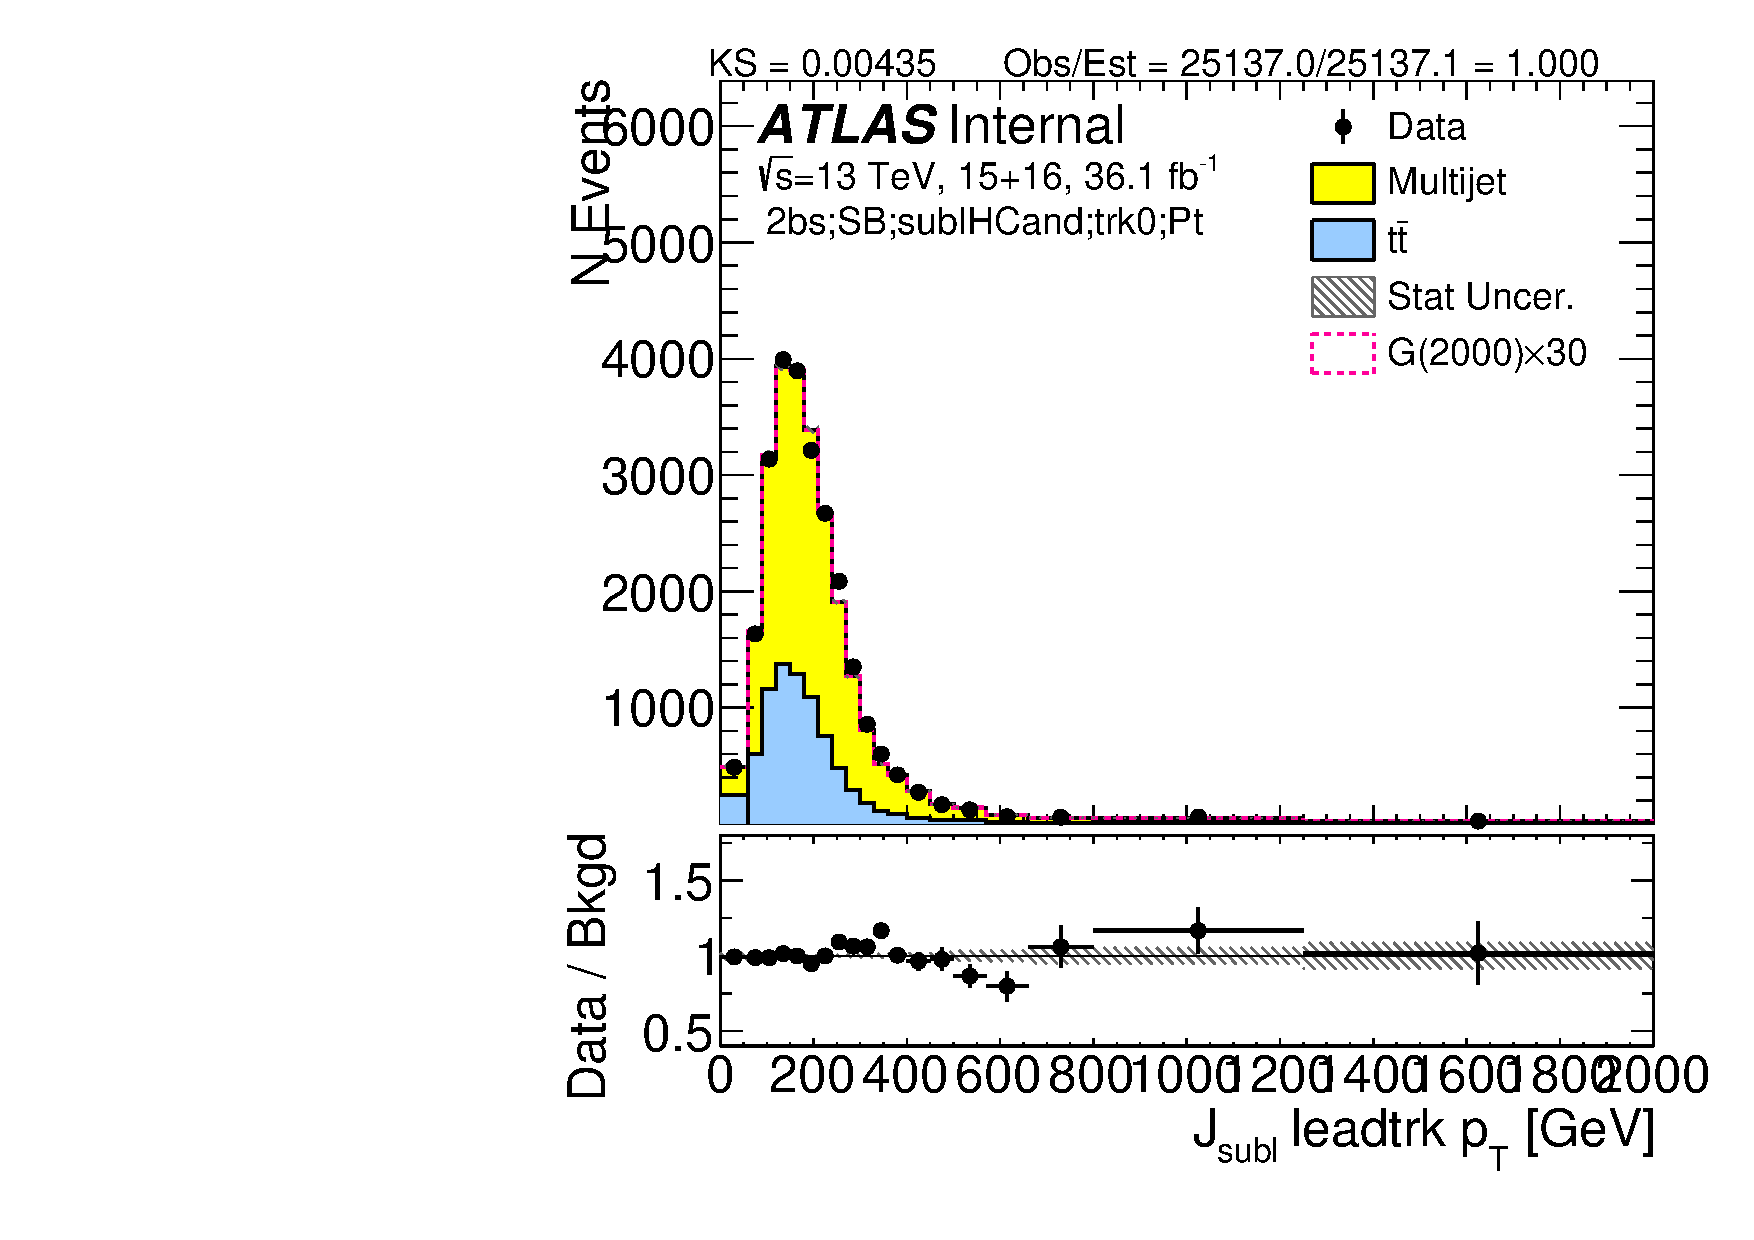
\includegraphics[width=0.32\textwidth,angle=-90]{figures/boosted/Sideband/b77_TwoTag_split_Sideband_sublHCand_trk0_Pt.pdf}
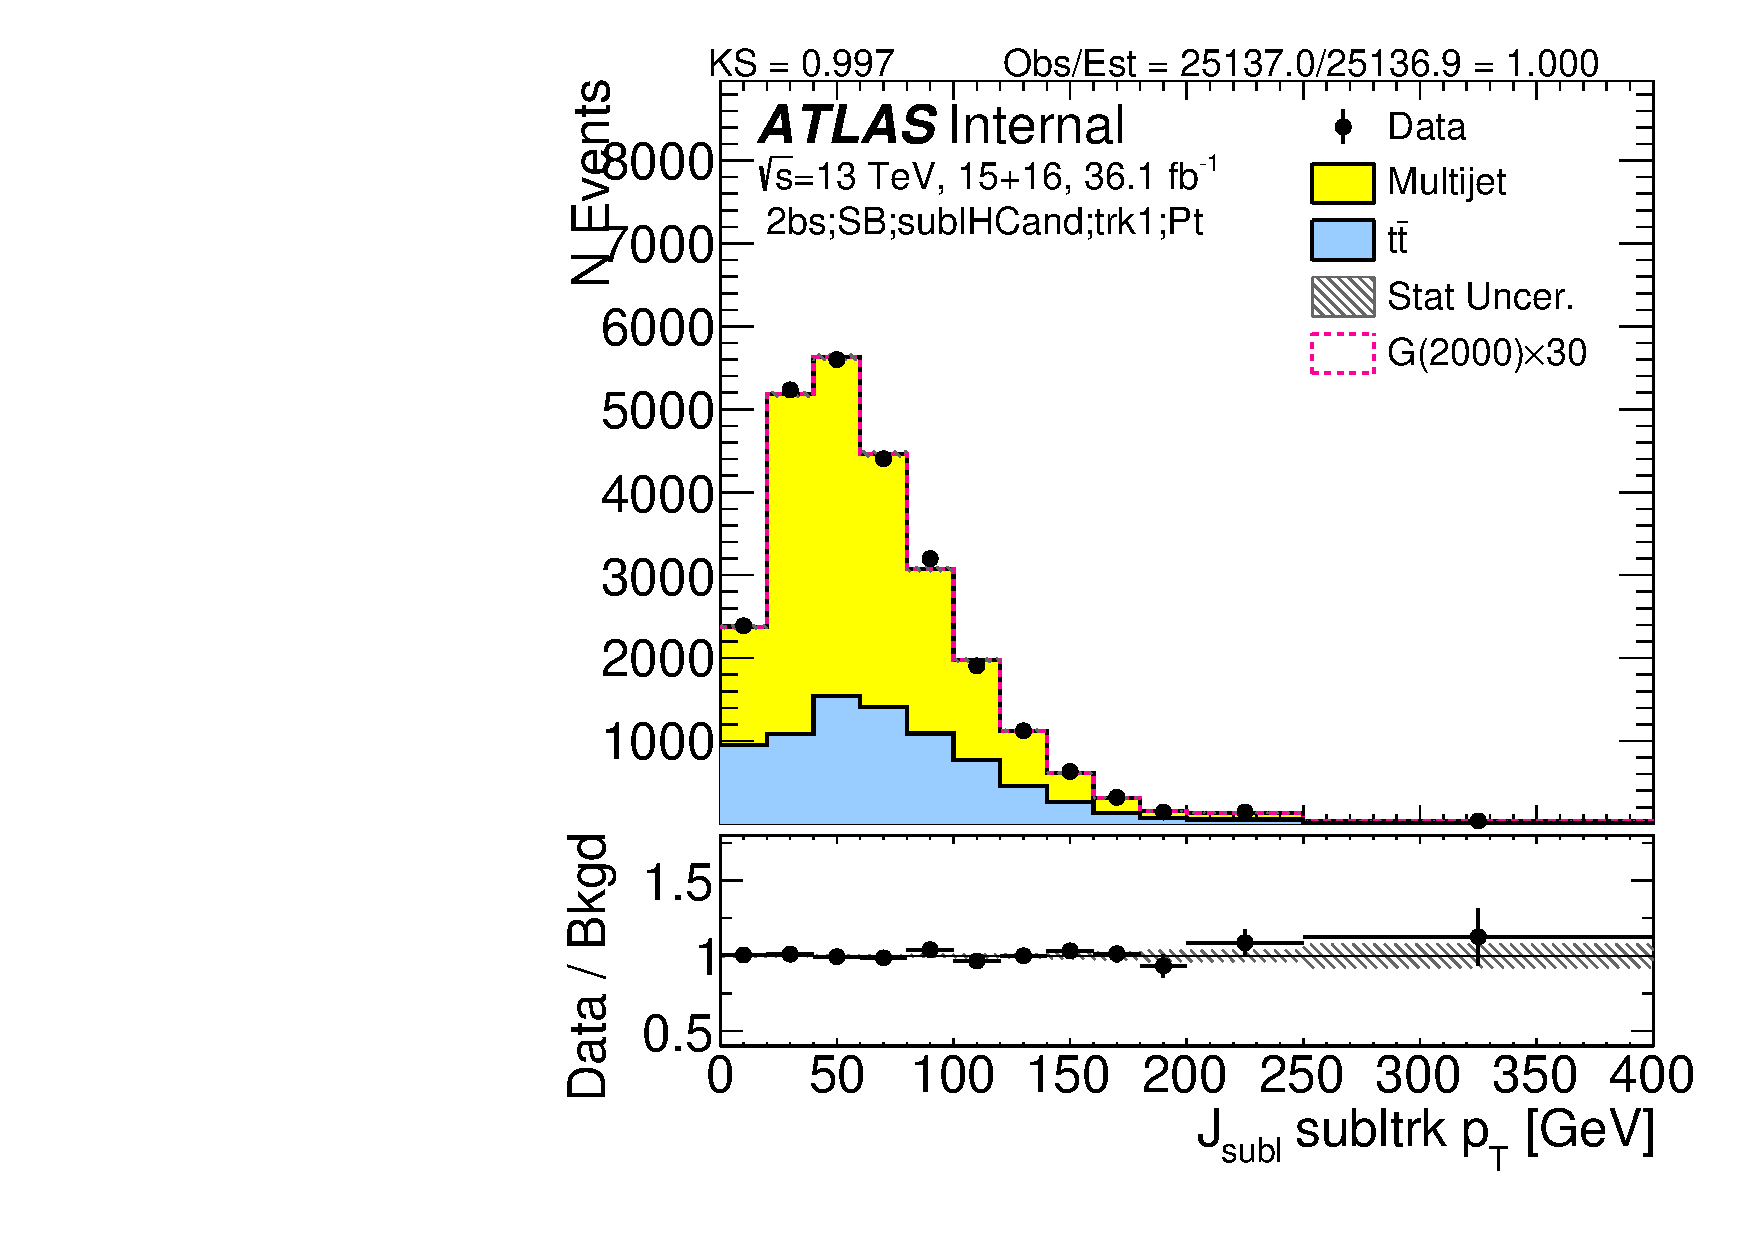
\includegraphics[width=0.32\textwidth,angle=-90]{figures/boosted/Sideband/b77_TwoTag_split_Sideband_sublHCand_trk1_Pt.pdf}\\
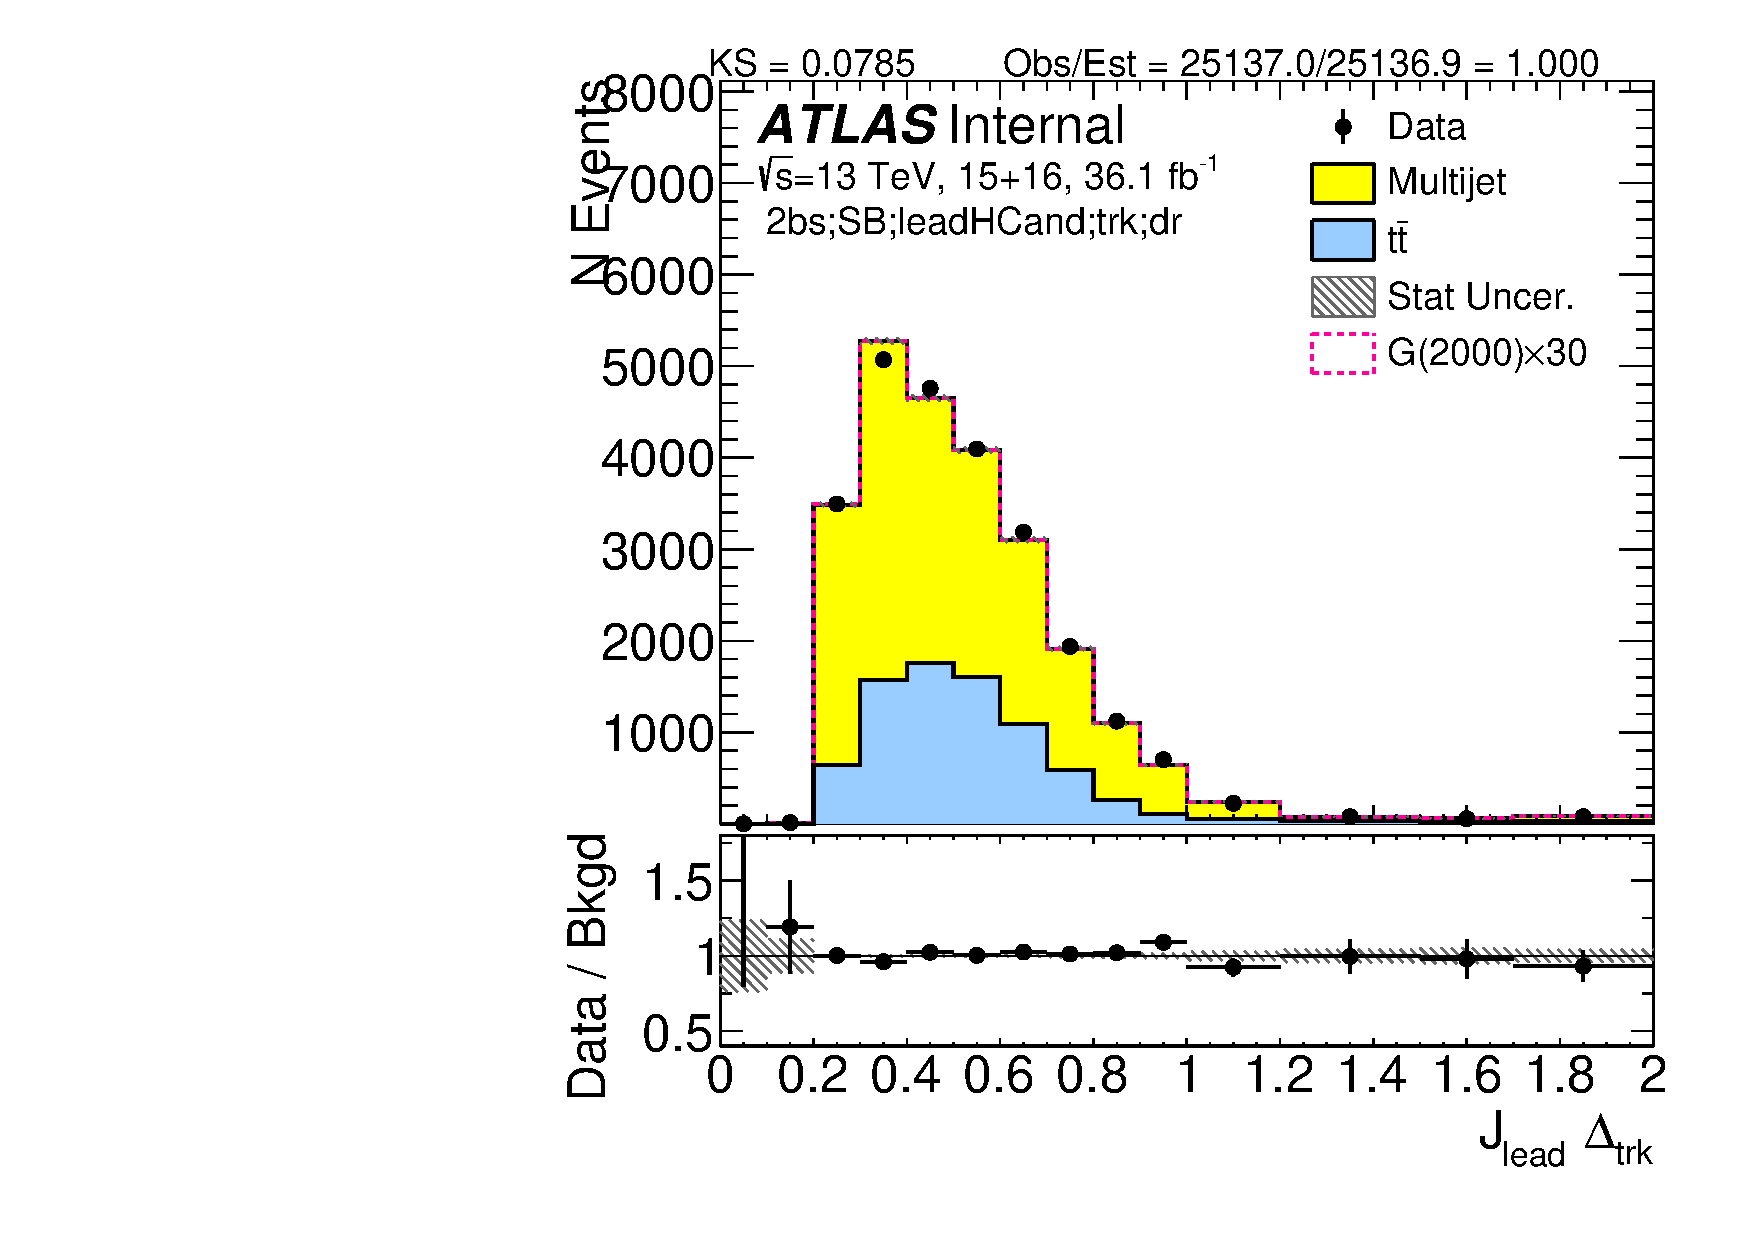
\includegraphics[width=0.32\textwidth,angle=-90]{figures/boosted/Sideband/b77_TwoTag_split_Sideband_leadHCand_trk_dr.pdf}
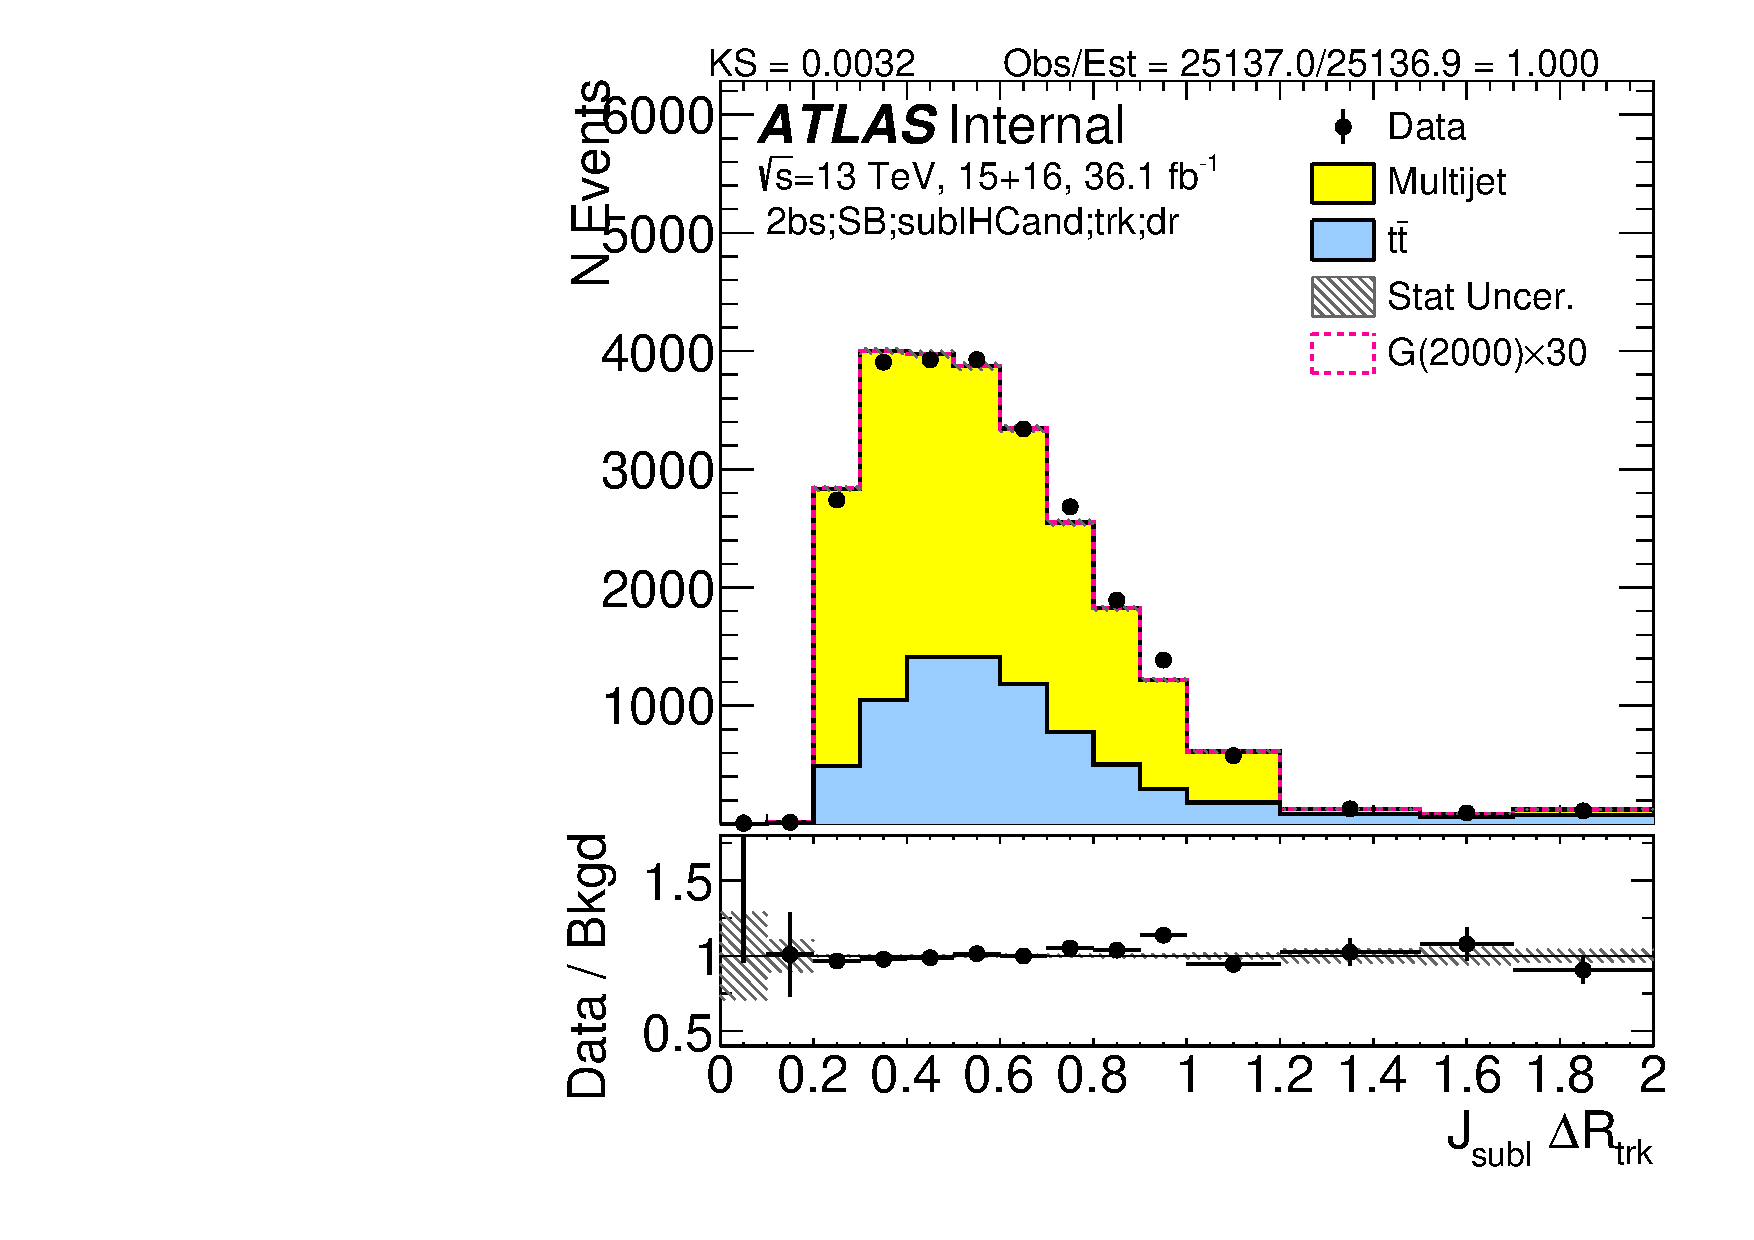
\includegraphics[width=0.32\textwidth,angle=-90]{figures/boosted/Sideband/b77_TwoTag_split_Sideband_sublHCand_trk_dr.pdf}
  \caption{First two rows show the \pt~ of the lead (left) and sub-lead (right) small-$R$ track jets associated to the lead (first-row) and sub-lead (second-row) large-\R jet in data and prediction in the sideband region after requiring 2 $b$-tags split. Third row shows the $\Delta R$ between two leading small-$R$ track-jets associated to the leading (left) and sub-leading (right) large-\R jet. }
  \label{fig:boosted-2bs-sideband-ak2}
\end{center}
\end{figure*}


\begin{figure*}[htbp!]
\begin{center}
\includegraphics[width=0.32\textwidth,angle=-90]{figures/boosted/Sideband/b77_TwoTag_split_Sideband_mHH_l_1.pdf}
\includegraphics[width=0.32\textwidth,angle=-90]{figures/boosted/Sideband/b77_TwoTag_split_Sideband_hCandDr.pdf}\\
\includegraphics[width=0.32\textwidth,angle=-90]{figures/boosted/Sideband/b77_TwoTag_split_Sideband_hCandDeta.pdf}
\includegraphics[width=0.32\textwidth,angle=-90]{figures/boosted/Sideband/b77_TwoTag_split_Sideband_hCandDphi.pdf}
  \caption{Kinematics (invariant mass, $\Delta R$, $\Delta \eta$ and $\Delta \phi$) of two large-\R jets in data and prediction in the sideband region after requiring 2 $b$-tags split. }
  \label{fig:boosted-2bs-sideband-ak10-system}
\end{center}
\end{figure*}

\clearpage
